% use font size 10pt for large document
% use font size  8pt for small document
\documentclass[a2paper,8pt]{extarticle}

% PARAMETER TO GREY OUT TEXT
\usepackage{etoolbox}
\newtoggle{greytext}
%\toggletrue{greytext}
\togglefalse{greytext}

% PARAMETER TO SHORTEN DOCUMENT
\newtoggle{shortdocument}
\toggletrue{shortdocument}
%\togglefalse{shortdocument}

% DECREASE LINE SPACING IF REQUESTED
\iftoggle{shortdocument}{
\setlength{\baselineskip}{0pt}
\renewcommand{\baselinestretch}{0.00001}
% TODO: next time: (better, but i have to use other equations)
%\setlength{\baselineskip}{1pt}
%\setlength{\lineskiplimit}{-16pt}
}

% PAPER LAYOUT
\iftoggle{shortdocument}{
\usepackage[margin=0.25cm,twoside]{geometry}
}{
\usepackage[margin=0.5cm,twoside
% TODO: activate if needed,bindingoffset=9mm
]{geometry}
}

% LANDSCAPE PACKAGE
\usepackage{pdflscape}

% TODO: page numbering
\usepackage{fancyhdr}
\pagestyle{fancy}
\renewcommand{\headrulewidth}{0pt}
\fancyfoot[C]{{\setlength\fboxsep{3pt}
\vspace*{-0.55cm}\colorbox{white}{\scriptsize\thepage}}}
\setlength{\footskip}{4pt}


% COMMENTS (invisible)
\usepackage{comment}

% COLORS
\usepackage{color}
\usepackage[dvipsnames]{xcolor}

% COLOR SHORTCUTS
\iftoggle{greytext}{
\newcommand{\tcr}[1]{\textcolor{lighttext}{#1}}
\newcommand{\tcb}[1]{\textcolor{lighttext}{#1}}
\newcommand{\tcg}[1]{\textcolor{lighttext}{#1}}
\newcommand{\tcgr}[1]{\textcolor{lighttext}{#1}}
\newcommand{\tcp}[1]{\textcolor{lighttext}{#1}}
}{
\newcommand{\tcr}[1]{\textcolor{red}{#1}}
\newcommand{\tcb}[1]{\textcolor{blue}{#1}}
\newcommand{\tcg}[1]{\textcolor{green}{#1}}
\newcommand{\tcp}[1]{\textcolor{pink}{#1}}
\newcommand{\tcgr}[1]{\textcolor{gray}{#1}}
}

% MULTICOLUMN LAYOUT
\usepackage{multicol}
\iftoggle{shortdocument}{
\setlength\columnsep{10pt}
}{
\setlength\columnsep{20pt}
}
\setlength{\columnseprule}{0.1pt}
\iftoggle{greytext}{
\renewcommand{\columnseprulecolor}{\color{lighttext}}
}{
}

% PARAGRAPH LAYOUT
\setlength\parindent{0pt}	% indentation
\setlength\parskip{2pt}		% space between paragraphs

% LANGUAGE SETTINGS
%\usepackage[ngerman]{babel} % Silbentrennung (und Deutsche Titel)
\usepackage[utf8]{inputenc} % Umlaute

% FONTS
%\usepackage{mathpazo}
%\usepackage{helvet}
%\usepackage{fouriernc}
%\usepackage[varg]{txfonts}
%\usepackage{mathptmx}
%\usepackage[charter]{mathdesign}
%\usepackage[garamond]{mathdesign}
%\usepackage[utopia]{mathdesign}
%\usepackage{fourier}
% font kerning (load after specific font!)
\usepackage{microtype}

% CUSTOM FONT SIZES
\usepackage{relsize}

% FIGURE SETTINGS
\usepackage{pict2e} % load this before picture
\usepackage{picture}
\usepackage{graphicx}
\usepackage{adjustbox}
\usepackage{caption}
\usepackage{subcaption}

% TIKZ GRAPHICS
\usepackage{tikz}
\usetikzlibrary{calc,matrix,arrows,automata,fit,shapes.multipart}
\tikzset{% 
    arr/.style={%
        -latex
    }
}
\tikzset{%
    var/.style={%
    	circle,draw=black
    }
}
\tikzset{%
	fac/.style={%
		rectangle,draw=black,align=center
	}
}
\newcommand{\fadeoutarr}[2]{%
\draw[] (#1) edge 
        ($(#1)!0.45!(#2)$) edge [dotted] 
        ($(#1)!0.75!(#2)$)
}
\newcommand{\fadeinarr}[2]{%
\draw[] ($(#1)!0.45!(#2)$) edge[dotted] 
        ($(#1)!0.75!(#2)$) edge[arr] 
        (#2) }
        
\newcommand{\tfactor}[4]{
\node[fac] (#1) at (#2) {{\tiny #4}\\#3};
}
\newcommand{\tnode}[3]{
\node[var] (#1) at (#2) {#3};
}
\newcommand{\tedge}[2]{
\draw[] (#1) edge (#2);
}
\newcommand{\tarrow}[2]{
\draw[arr] (#1) edge (#2);
}
\usepackage{tikz-cd}

% SIMPLE TREES
\usepackage{qtree}

% PLOTS
\usepackage{pgfplots}
\pgfplotsset{compat=1.10}

% FLOAT SETTINGS
\usepackage{float}

% REFERENCING
\usepackage{hyperref}

% TABLES
\usepackage{booktabs} % nicer tables
\usepackage{makecell}
\usepackage{array} % custom column types
\usepackage{multirow} % span cells over multiple rows
\newcommand{\tabitem}{~~\llap{{\boldmath $\cdot$}}~} % items in tables

% LISTS
\usepackage{enumitem}
\setlist{noitemsep,topsep=0pt,parsep=0pt,partopsep=0pt,leftmargin=10pt}
\renewcommand\labelitemi{{\boldmath$\cdot$}}
\renewcommand\labelitemii{{\boldmath$\cdot$}}
\renewcommand\labelitemiii{{\boldmath$\cdot$}}
% advantages disadvantages
\newcommand\pro{\item[$+$]}
\newcommand\con{\item[$-$]}

% TIGHT CENTER ENVIRONMENT
\newenvironment{tightcenter}{%
  \begin{center}
  \vspace{-12pt}
}{
  \vspace{-12pt}
  \end{center}
}

% COMMAND TO ROTATE MATH SYMBOLS
\newcommand{\rot}[2]{\rotatebox[origin=c]{#1}{#2}}

% MATH (packages and settings)
\usepackage{blkarray}  		% matrix annotations
\usepackage[intlimits]{mathtools}
\usepackage{amsfonts}
\usepackage{bm}
\usepackage{amssymb}
\usepackage{wasysym}
\usepackage{ifsym}
\usepackage{dsfont}
\usepackage{resizegather} 	% resizing equations
\usepackage{oubraces}    	% special overlapping over/underbraces
\usepackage{scalerel}		% scaling of characters
\usepackage{cancel}			% crossing out of terms
\allowdisplaybreaks 		% allow page break in align* environment

% PROOF TREES
\usepackage{proof}
\inferLineSkip=4pt % adjust line skip between proofs

% PROOFS
\newcommand{\qed}{\hfill$\square$}
\newcommand{\contradiction}{\hfill$\lightning$}

% MATH HIGHLIGHTING
\newcommand{\mhl}[2]{\colorbox{#1}{$\displaystyle#2$}}
\newcommand{\mhlr}[1]{\mathhl{red}{#1}}
\newcommand{\mhlg}[1]{\mathhl{green}{#1}}
\newcommand{\mhlb}[1]{\mathhl{blue}{#1}}
\newcommand{\mhly}[1]{\mathhl{yellow}{#1}}

% CODE IN MATH
\newcommand{\mcode}[1]{{\normalfont\texttt{\textbf{#1}}}}

% COLOR IN MATH (without the bad behaviour of textcolor)
\makeatletter
\def\mc#1#{\@mc{#1}}
\def\@mc#1#2#3{%
  \protect\leavevmode
  \begingroup
    \color#1{#2}#3%
  \endgroup
}
\makeatother

\iftoggle{greytext}{
\definecolor{brilliantrose}{rgb}{1.0, 0.33, 0.64}
\newcommand{\mcr}[1]{\mc{lighttext}{#1}}
\newcommand{\mcg}[1]{\mc{lighttext}{#1}}
\newcommand{\mcb}[1]{\mc{lighttext}{#1}}
\newcommand{\mcy}[1]{\mc{lighttext}{#1}}
\newcommand{\mcp}[1]{\mc{lighttext}{#1}}
\newcommand{\mcw}[1]{\mc{white}{#1}}
\newcommand{\mcgr}[1]{\mc{lighttext}{#1}}
}{
\definecolor{brilliantrose}{rgb}{1.0, 0.33, 0.64}
\newcommand{\mcr}[1]{\mc{red}{#1}}
\newcommand{\mcg}[1]{\mc{green}{#1}}
\newcommand{\mcb}[1]{\mc{blue}{#1}}
\newcommand{\mcy}[1]{\mc{yellow}{#1}}
\newcommand{\mcp}[1]{\mc{brilliantrose}{#1}}
\newcommand{\mcw}[1]{\mc{white}{#1}}
\newcommand{\mcgr}[1]{\mc{gray}{#1}}
}

% ASYMPTOTIC NOTATIONS
\newcommand{\BigO}{\mathcal{O}}

% NUMBER SYSTEMS
\newcommand{\A}{\mathbb{A}}
\newcommand{\B}{\mathbb{B}}
\newcommand{\C}{\mathbb{C}}
\newcommand{\D}{\mathbb{D}}
\newcommand{\E}{\mathbb{E}}
\newcommand{\F}{\mathbb{F}}
\newcommand{\G}{\mathbb{G}}
\newcommand{\bbH}{\mathbb{H}}
\newcommand{\I}{\mathbb{I}}
\newcommand{\J}{\mathbb{J}}
\newcommand{\K}{\mathbb{K}}
\newcommand{\bbL}{\mathbb{L}}
\newcommand{\M}{\mathbb{M}}
\newcommand{\N}{\mathbb{N}}
\newcommand{\bbO}{\mathbb{O}}
\newcommand{\bbP}{\mathbb{P}}
\newcommand{\Q}{\mathbb{Q}}
\newcommand{\R}{\mathbb{R}}
\newcommand{\bbS}{\mathbb{S}}
\newcommand{\bbT}{\mathbb{T}}
\newcommand{\U}{\mathbb{U}}
\newcommand{\V}{\mathbb{V}}
\newcommand{\W}{\mathbb{W}}
\newcommand{\X}{\mathbb{X}}
\newcommand{\Y}{\mathbb{Y}}
\newcommand{\Z}{\mathbb{Z}}

% CALLICGRAPHIC SHORTCUTS
\newcommand{\cA}{\mathcal{A}}
\newcommand{\cB}{\mathcal{B}}
\newcommand{\cC}{\mathcal{C}}
\newcommand{\cD}{\mathcal{D}}
\newcommand{\cE}{\mathcal{E}}
\newcommand{\cF}{\mathcal{F}}
\newcommand{\cG}{\mathcal{G}}
\newcommand{\cH}{\mathcal{H}}
\newcommand{\cI}{\mathcal{I}}
\newcommand{\cJ}{\mathcal{J}}
\newcommand{\cK}{\mathcal{K}}
\newcommand{\cL}{\mathcal{L}}
\newcommand{\cM}{\mathcal{M}}
\newcommand{\cN}{\mathcal{N}}
\newcommand{\cO}{\mathcal{O}}
\newcommand{\cP}{\mathcal{P}}
\newcommand{\cQ}{\mathcal{Q}}
\newcommand{\cR}{\mathcal{R}}
\newcommand{\cS}{\mathcal{S}}
\newcommand{\cT}{\mathcal{T}}
\newcommand{\cU}{\mathcal{U}}
\newcommand{\cV}{\mathcal{V}}
\newcommand{\cW}{\mathcal{W}}
\newcommand{\cX}{\mathcal{X}}
\newcommand{\cY}{\mathcal{Y}}
\newcommand{\cZ}{\mathcal{Z}}

% BRACES
\newcommand{\set}[1]{\left\{ #1 \right\}}
\newcommand{\dset}[2]{\left\{ #1 \ \middle| \ #2 \right\}}
\newcommand{\alg}[1]{\left\langle #1 \right\rangle}
\newcommand{\card}[1]{\left\lvert #1 \right\rvert}
\newcommand{\length}[1]{\left\lvert #1 \right\rvert}
\newcommand{\abs}[1]{\left\lvert #1 \right\rvert}
\newcommand{\norm}[1]{\left\lVert #1 \right\rVert}
\newcommand{\scprod}[1]{\left\langle #1 \right\rangle}
\newcommand{\ceil}[1]{\left\lceil #1 \right\rceil}
\newcommand{\floor}[1]{\left\lfloor #1 \right\rfloor}
\newcommand{\linsys}[2]{\left[\ #1 \ \middle| \ #2 \ \right]}
\newcommand{\Sim}[1]{\text{Sim}\left( #1 \right)}
\newcommand{\Tr}[1]{\mathsf{Tr}\left( #1 \right)}
\newcommand{\sTr}[1]{\mathsf{Tr}( #1 )}

% BRACES SMALL (no adjusting)
\newcommand{\sset}[1]{\{ #1 \}}
\newcommand{\sdset}[2]{\{ #1 \ | \ #2 \}}
\newcommand{\salg}[1]{\langle #1 \rangle}
\newcommand{\scard}[1]{\lvert #1 \rvert}
\newcommand{\slength}[1]{\lvert #1 \rvert}
\newcommand{\sabs}[1]{\lvert #1 \rvert}
\newcommand{\snorm}[1]{\lVert #1 \rVert}
\newcommand{\sscprod}[1]{\langle #1 \rangle}
\newcommand{\sceil}[1]{\lceil #1 \rceil}
\newcommand{\sfloor}[1]{\lfloor #1 \rfloor}
\newcommand{\slinsys}[2]{[\ #1 \ | \ #2 \ ]}
\newcommand{\sSim}[1]{\text{Sim}( #1 )}

% OPERATORS
\newcommand{\conv}{\ensuremath *}

% EMPTY SET
\let\oldemptyset\emptyset
\let\emptyset\varnothing

% NOT IN SHORTCUT
\newcommand{\nin}{\not\in}

% DISJOINT UNION SYMBOL
\makeatletter
\def\moverlay{\mathpalette\mov@rlay}
\def\mov@rlay#1#2{\leavevmode\vtop{%
   \baselineskip\z@skip \lineskiplimit-\maxdimen
   \ialign{\hfil$\m@th#1##$\hfil\cr#2\crcr}}}
\newcommand{\charfusion}[3][\mathord]{
    #1{\ifx#1\mathop\vphantom{#2}\fi
        \mathpalette\mov@rlay{#2\cr#3}
      }
    \ifx#1\mathop\expandafter\displaylimits\fi}
\makeatother
\newcommand{\bigcupdot}{\charfusion[\mathop]{\bigcup}{\cdot}}
\newcommand{\cupdot}{\mathbin{\mathaccent\cdot\cup}}

% CUSTOM STATISTICS
\newcommand{\Prob}[2][]{P_{#1}\left( #2 \right)}
\newcommand{\cProb}[3][]{P_{#1}\left( #2 \,\middle|\, #3 \right)}
\newcommand{\Dist}[2]{#1\left( #2 \right)}
\newcommand{\cDist}[3]{#1\left( #2 \,\middle|\, #3 \right)}
\newcommand{\hProb}[2][]{\hat{P}_{#1}\left( #2 \right)}
\newcommand{\chProb}[2]{\hat{P}\left( #1 \,\middle|\, #2 \right)}
\newcommand{\Var}[2][]{\operatorname{Var}_{#1}\left[ #2 \right]}
\newcommand{\sd}[1]{\operatorname{sd}\left( #1 \right)}
\newcommand{\Exp}[2][]{{\mathbb{E}_{#1}}\left[ #2
\right]}
\newcommand{\cExp}[3][]{{\mathbb{E}}_{#1}\left[ #2
\,\middle|\, #3 \right]}
\newcommand{\hExp}[2][]{{\mathbb{\hat{E}}_{#1}}\left[ #2
\right]}
\newcommand{\chExp}[3][]{{\mathbb{\hat{E}}}_{#1}\left[ #2
\,\middle|\, #3 \right]}
\newcommand{\Corr}[1]{\operatorname{Corr}\left[ #1 \right]}
\newcommand{\Cov}[1]{\operatorname{Cov}\left(#1 \right)}
\newcommand{\MSE}[2][]{\operatorname{MSE}_{#1}\left[ #2 \right]}
\newcommand{\riid}{\stackrel{\text{\tiny i.i.d.}}{\sim}}
\newcommand{\approxsim}{\stackrel{\text{approx.}}{\sim}}
\newcommand{\ind}[1]{\mathds{1}_{\set{#1}}}
\newcommand{\eqiid}{\stackrel{\text{\tiny i.i.d.}}{=}}
\newcommand{\eqind}{\stackrel{\text{\tiny ind.}}{=}}

% BAYESIAN NETWORKS
\newcommand{\indep}{\perp}
\newcommand{\given}{\,\,|\,\,}
\newcommand{\Pa}{\mathbf{Pa}}
\newcommand{\dsep}[2]{\operatorname{d-sep}\left( #1 \,\middle|\, #2 \right)}

% RANDOM VARIABLES
\newcommand{\rA}{A}
\newcommand{\rB}{B}
\newcommand{\rC}{C}
\newcommand{\rD}{D}
\newcommand{\rE}{E}
\newcommand{\rF}{F}
\newcommand{\rG}{G}
\newcommand{\rH}{H}
\newcommand{\rI}{I}
\newcommand{\rJ}{J}
\newcommand{\rK}{K}
\newcommand{\rL}{L}
\newcommand{\rM}{M}
\newcommand{\rN}{N}
\newcommand{\rO}{O}
\newcommand{\rP}{P}
\newcommand{\rQ}{Q}
\newcommand{\rR}{R}
\newcommand{\rS}{S}
\newcommand{\rT}{T}
\newcommand{\rU}{U}
\newcommand{\rV}{V}
\newcommand{\rW}{W}
\newcommand{\rX}{X}
\newcommand{\rY}{Y}
\newcommand{\rZ}{Z}

% RANDOM VECTORS
% declares a custom italic bold alphabet for random vectors
\DeclareMathAlphabet{\mathbfit}{OML}{cmm}{b}{it}
\newcommand{\rvA}{\mathbfit{A}}
\newcommand{\rvB}{\mathbfit{B}}
\newcommand{\rvC}{\mathbfit{C}}
\newcommand{\rvD}{\mathbfit{D}}
\newcommand{\rvE}{\mathbfit{E}}
\newcommand{\rvF}{\mathbfit{F}}
\newcommand{\rvG}{\mathbfit{G}}
\newcommand{\rvH}{\mathbfit{H}}
\newcommand{\rvI}{\mathbfit{I}}
\newcommand{\rvJ}{\mathbfit{J}}
\newcommand{\rvK}{\mathbfit{K}}
\newcommand{\rvL}{\mathbfit{L}}
\newcommand{\rvM}{\mathbfit{M}}
\newcommand{\rvN}{\mathbfit{N}}
\newcommand{\rvO}{\mathbfit{O}}
\newcommand{\rvP}{\mathbfit{P}}
\newcommand{\rvQ}{\mathbfit{Q}}
\newcommand{\rvR}{\mathbfit{R}}
\newcommand{\rvS}{\mathbfit{S}}
\newcommand{\rvT}{\mathbfit{T}}
\newcommand{\rvU}{\mathbfit{U}}
\newcommand{\rvV}{\mathbfit{V}}
\newcommand{\rvW}{\mathbfit{W}}
\newcommand{\rvX}{\mathbfit{X}}
\newcommand{\rvY}{\mathbfit{Y}}
\newcommand{\rvZ}{\mathbfit{Z}}

% MACHINE LEARNING
\newcommand{\Risk}[1]{R\left(#1\right)}
\newcommand{\empRisk}[1]{\widehat{R}\left(#1\right)}

% ACCENTS
% TODO: fix this, make spacing nice
\newcommand*{\Hm}{\mathsf{H}}
\newcommand*{\T}{\mathsf{T}}
%\newcommand*{\T}{\mkern-1mu{}_{}^{\scriptscriptstyle\top}\mkern-4mu}
\newcommand*{\Rev}{\mathsf{R}}
\newcommand{\conj}[1]{\overline{ #1 }}

% CUSTOM ALPHABETS
\renewcommand{\S}{\Sigma}
\newcommand{\Ss}{\Sigma^*}
\newcommand{\Sp}{\Sigma^+}
\newcommand{\Sbool}{\Sigma_{\text{bool}}}
\newcommand{\Ssbool}{(\Sigma_{\text{bool}})^*}
\newcommand{\Slogic}{\Sigma_{\text{logic}}}
\newcommand{\Sslogic}{(\Sigma_{\text{logic}})^*}
\newcommand{\Slat}{\Sigma_{\text{lat}}}
\newcommand{\Sslat}{(\Sigma_{\text{lat}})^*}
\newcommand{\Stastatur}{\Sigma_{\text{Tastatur}}}
\newcommand{\Sstastatur}{(\Sigma_{\text{Tastatur}})^*}
\newcommand{\Sm}{\Sigma_{m}}
\newcommand{\Ssm}{\Sigma_{m}^*}
\newcommand{\ZO}{\{0,1\}}
\newcommand{\ZOs}{\{0,1\}^*}
\newcommand{\hdelta}{\hat\delta}

% OPERATORS
% TODO: Should I design these as braces?
\DeclareMathOperator{\id}{\text{id}}
\DeclareMathOperator{\Kon}{\text{Kon}}
\DeclareMathOperator{\cost}{\text{cost}}
\DeclareMathOperator{\goal}{\text{goal}}
\DeclareMathOperator{\Opt}{\text{Opt}}
\DeclareMathOperator{\Bin}{\text{Bin}}
\DeclareMathOperator{\Nummer}{\text{Nummer}}
\DeclareMathOperator{\Prim}{\text{Prim}}
\DeclareMathOperator{\Kl}{\text{Kl}}
\DeclareMathOperator{\lcm}{lcm}
\DeclareMathOperator{\glb}{glb}
\DeclareMathOperator{\lub}{lub}
\DeclareMathOperator{\im}{im}
\DeclareMathOperator{\ord}{ord}
\DeclareMathOperator{\rank}{rank}
\DeclareMathOperator{\spn}{span}
\DeclareMathOperator{\Cost}{Cost}
\DeclareMathOperator{\order}{order}
\DeclareMathOperator{\dist}{dist}
\DeclareMathOperator{\cond}{cond}
\DeclareMathOperator{\nnz}{nnz}
\DeclareMathOperator{\sign}{sign}
\DeclareMathOperator{\Count}{Count}
\DeclareMathOperator{\Spur}{Spur}
\DeclareMathOperator{\triu}{triu}
\DeclareMathOperator{\cumsum}{cumsum}
\DeclareMathOperator{\vectorize}{vectorize}
\DeclareMathOperator{\matrixfy}{matrixfy}
\DeclareMathOperator{\circul}{circul}
\DeclareMathOperator{\dft}{dft}
\DeclareMathOperator{\invdft}{invdft}
\DeclareMathOperator{\ones}{ones}
\DeclareMathOperator{\arcsinh}{arcsinh}
\DeclareMathOperator{\arccosh}{arccosh}
\DeclareMathOperator{\arctanh}{arctanh}
\let\division\div
\renewcommand\div{\operatorname{div}}
\DeclareMathOperator{\cis}{cis}
\DeclareMathOperator{\grad}{grad}
\DeclareMathOperator{\Hess}{Hess}
\newcommand{\laplace}{\Delta}
\DeclareMathOperator*{\argmin}{arg\,min}
\DeclareMathOperator*{\argmax}{arg\,max}
\DeclareMathOperator{\odd}{odd}
\DeclareMathOperator{\even}{even}
\DeclareMathOperator{\Proj}{Proj}
\DeclareMathOperator{\softmax}{\text{softmax}}
\DeclareMathOperator{\ReLU}{\text{ReLU}}
\DeclareMathOperator{\pmi}{\text{pmi}}

% TODO: fix these operator braces
% TODO: think about which ones should have braces
% and which one shouldn't. E.g., a function might need derivatives '
% or it might be used without argument, just in compositions \circ
\newcommand{\diag}{\text{diag}}

% CRYPTOGRAPHY
\DeclareMathOperator{\concat}{ || }
\DeclareMathOperator{\Enc}{Enc}
\DeclareMathOperator{\Dec}{Dec}
\DeclareMathOperator{\Gen}{Gen}
\DeclareMathOperator{\Tag}{Tag}
\DeclareMathOperator{\Vrfy}{Vrfy}
\DeclareMathOperator{\MAC}{\text{MAC}}
\newcommand{\AdvPRG}[2][]{\text{Adv}_{\text{PRG}}\left[ #2 \right]}
\newcommand{\yes}{\text{yes}}
\newcommand{\no}{\text{no}}
\newcommand{\forallPPTTM}{%
\underset{\mathclap{\substack{\text{\tiny prob. poly-}\\
\text{\tiny time TM}}}}{\forall}}
\newcommand{\forallPTAdv}{%
\underset{\mathclap{\substack{\text{\tiny poly-time}\\
\text{\tiny Adversaries}}}}{\forall}}

% OPERATORS (OVERRIDDEN)
\renewcommand\Re{\operatorname{Re}}
\renewcommand\Im{\operatorname{Im}}

% RELATIONAL ALGEBRA
\renewcommand{\setminus}{-} 
\DeclareMathOperator{\dom}{dom}
\DeclareMathOperator{\sch}{sch}
\newcommand{\dto}{\stackrel{\bullet}{\to}}
%\newcommand{\join}{\bowtie}
%\newcommand{\lojoin}{\,{\tiny \textifsym{d|><|}}\,}
%\newcommand{\rojoin}{\,{\tiny \textifsym{|><|d}}\,}
%\newcommand{\fojoin}{\,{\tiny \textifsym{d|><|d}}\,}
%\newcommand{\lsjoin}{\ltimes}
%\newcommand{\rsjoin}{\rtimes}

\newcommand{\fojoin}{
\,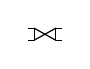
\begin{tikzpicture}%
% bowtie - X
\draw[line width=0.15mm,line cap=round] (0,0) -- (1.8ex,1ex);
\draw[line width=0.15mm,line cap=round] (0,1ex) -- (1.8ex,0ex);
% bowtie - side left
\draw[line width=0.15mm,line cap=round] (0,0) -- (0,1ex);
% bowtie - side right
\draw[line width=0.15mm,line cap=round] (1.8ex,0) -- (1.8ex,1ex);
% left wedges
\draw[line width=0.15mm] (0,0) -- (-0.5ex,0);
\draw[line width=0.15mm] (0,1ex) -- (-0.5ex,1ex);
% right wedges
\draw[line width=0.15mm] (1.8ex,0) -- (2.3ex,0);
\draw[line width=0.15mm] (1.8ex,1ex) -- (2.3ex,1ex);
\end{tikzpicture}\,
}

\newcommand{\join}{
\,
\begin{tikzpicture}%
% bowtie - X
\draw[line width=0.15mm,line cap=round] (0,0) -- (1.8ex,1ex);
\draw[line width=0.15mm,line cap=round] (0,1ex) -- (1.8ex,0ex);
% bowtie - side left
\draw[line width=0.15mm,line cap=round] (0,0) -- (0,1ex);
% bowtie - side right
\draw[line width=0.15mm,line cap=round] (1.8ex,0) -- (1.8ex,1ex);
\end{tikzpicture}\,
}

\newcommand{\lojoin}{
\,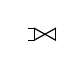
\begin{tikzpicture}%
% bowtie - X
\draw[line width=0.15mm,line cap=round] (0,0) -- (1.8ex,1ex);
\draw[line width=0.15mm,line cap=round] (0,1ex) -- (1.8ex,0ex);
% bowtie - side left
\draw[line width=0.15mm,line cap=round] (0,0) -- (0,1ex);
% bowtie - side right
\draw[line width=0.15mm,line cap=round] (1.8ex,0) -- (1.8ex,1ex);
% left wedges
\draw[line width=0.15mm] (0,0) -- (-0.5ex,0);
\draw[line width=0.15mm] (0,1ex) -- (-0.5ex,1ex);
\end{tikzpicture}\,
}

\newcommand{\rojoin}{
\,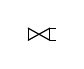
\begin{tikzpicture}%
% bowtie - X
\draw[line width=0.15mm,line cap=round] (0,0) -- (1.8ex,1ex);
\draw[line width=0.15mm,line cap=round] (0,1ex) -- (1.8ex,0ex);
% bowtie - side left
\draw[line width=0.15mm,line cap=round] (0,0) -- (0,1ex);
% bowtie - side right
\draw[line width=0.15mm,line cap=round] (1.8ex,0) -- (1.8ex,1ex);
% right wedges
\draw[line width=0.15mm] (1.8ex,0) -- (2.3ex,0);
\draw[line width=0.15mm] (1.8ex,1ex) -- (2.3ex,1ex);
\end{tikzpicture}\,
}

\newcommand{\lsjoin}{
\,
\begin{tikzpicture}%
% bowtie - X
\draw[line width=0.15mm,line cap=round] (0,0) -- (1.8ex,1ex);
\draw[line width=0.15mm,line cap=round] (0,1ex) -- (1.8ex,0ex);
% bowtie - side left
\draw[line width=0.15mm,line cap=round] (0,0) -- (0,1ex);
\end{tikzpicture}\,
}


\newcommand{\rsjoin}{
\,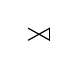
\begin{tikzpicture}%
% bowtie - X
\draw[line width=0.15mm,line cap=round] (0,0) -- (1.8ex,1ex);
\draw[line width=0.15mm,line cap=round] (0,1ex) -- (1.8ex,0ex);
% bowtie - side right
\draw[line width=0.15mm,line cap=round] (1.8ex,0) -- (1.8ex,1ex);
\end{tikzpicture}\,
}

% RELATIONS
\newcommand{\mbeq}{\stackrel{!}{=}}
\newcommand{\xor}{\mathrel{\text{xor}}}
\newcommand{\relid}{\mathrel{\id}}
\newcommand{\relrho}{\mathrel{\rho}}
\newcommand{\relsigma}{\mathrel{\sigma}}
\newcommand{\reltheta}{\mathrel{\theta}}
\newcommand{\relsim}{\mathrel{\sim}}
\newcommand{\relf}{\mathrel{f}}

% RELATIONS (INVERSES)
\newcommand{\invrelid}{\mathrel{\widehat{\id}}}
\newcommand{\invrelrho}{\mathrel{\widehat{\rho}}}
\newcommand{\invrelsigma}{\mathrel{\widehat{\sigma}}}
\newcommand{\invreltheta}{\mathrel{\widehat{\theta}}}
\newcommand{\invrelsim}{\mathrel{\widehat{\sim}}}
\newcommand{\invrelf}{\mathrel{\widehat{f}}}

% CUSTOM RELATIONS
\DeclareRobustCommand{\step}[2][]{\mathrel{\drawstep{#1}{#2}}}
\newcommand{\drawstep}[2]{%
  \vcenter{\hbox{%
    \setlength{\unitlength}{1em}%
    \begin{picture}(1,1)
    \roundcap
    \put(0,0){\line(0,1){1}}
    \put(0,0.5){\line(1,0){0.95}}
    \put(0.5,0){\makebox[0pt]{\text{\smaller$\scriptscriptstyle#2$}}}
    \put(0.5,0.6){\makebox[0pt]{\text{\smaller$#1$}}}
    \end{picture}%
  }}%
}

% LINEAR TEMPORAL LOGIC (LTL)
\newcommand{\until}{\texttt{\,\hstretch{0.7}{\boldsymbol{\cup}}\,}}
\newcommand{\next}{\Circle}
\newcommand{\eventually}{\Diamond}
\newcommand{\always}{\square}

% GLOBAL MATRICES AND VECTOR SETTINGS
\newcommand{\boldm}[1] {\mathversion{bold}#1\mathversion{normal}}
\newcommand{\mat}[1]{\mathbf{#1}}
\renewcommand{\vec}[1]{\mathbf{#1}}

% VECTORS (LATIN)
\newcommand{\va}{\vec{a}}
\newcommand{\vb}{\vec{b}}
\newcommand{\vc}{\vec{c}}
\newcommand{\vd}{\vec{d}}
\newcommand{\ve}{\vec{e}}
\newcommand{\vf}{\vec{f}}
\newcommand{\vg}{\vec{g}}
\newcommand{\vh}{\vec{h}}
\newcommand{\vi}{\vec{i}}
\newcommand{\vj}{\vec{j}}
\newcommand{\vk}{\vec{k}}
\newcommand{\vl}{\vec{l}}
\newcommand{\vm}{\vec{m}}
\newcommand{\vn}{\vec{n}}
\newcommand{\vo}{\vec{o}}
\newcommand{\vp}{\vec{p}}
\newcommand{\vq}{\vec{q}}
\newcommand{\vr}{\vec{r}}
\newcommand{\vs}{\vec{s}}
\newcommand{\vt}{\vec{t}}
\newcommand{\vu}{\vec{u}}
\newcommand{\vv}{\vec{v}}
\newcommand{\vw}{\vec{w}}
\newcommand{\vx}{\vec{x}}
\newcommand{\vy}{\vec{y}}
\newcommand{\vz}{\vec{z}}

% VECTORS (LATIN) WITH TILDE ACCENT
\newcommand{\vta}{\widetilde{\vec{a}}}
\newcommand{\vtb}{\widetilde{\vec{b}}}
\newcommand{\vtc}{\widetilde{\vec{c}}}
\newcommand{\vtd}{\widetilde{\vec{d}}}
\newcommand{\vte}{\widetilde{\vec{e}}}
\newcommand{\vtf}{\widetilde{\vec{f}}}
\newcommand{\vtg}{\widetilde{\vec{g}}}
\newcommand{\vth}{\widetilde{\vec{h}}}
\newcommand{\vti}{\widetilde{\vec{i}}}
\newcommand{\vtj}{\widetilde{\vec{j}}}
\newcommand{\vtk}{\widetilde{\vec{k}}}
\newcommand{\vtl}{\widetilde{\vec{l}}}
\newcommand{\vtm}{\widetilde{\vec{m}}}
\newcommand{\vtn}{\widetilde{\vec{n}}}
\newcommand{\vto}{\widetilde{\vec{o}}}
\newcommand{\vtp}{\widetilde{\vec{p}}}
\newcommand{\vtq}{\widetilde{\vec{q}}}
\newcommand{\vtr}{\widetilde{\vec{r}}}
\newcommand{\vts}{\widetilde{\vec{s}}}
\newcommand{\vtt}{\widetilde{\vec{t}}}
\newcommand{\vtu}{\widetilde{\vec{u}}}
\newcommand{\vtv}{\widetilde{\vec{v}}}
\newcommand{\vtw}{\widetilde{\vec{w}}}
\newcommand{\vtx}{\widetilde{\vec{x}}}
\newcommand{\vty}{\widetilde{\vec{y}}}
\newcommand{\vtz}{\widetilde{\vec{z}}}

% VECTORS (LATIN) WITH HAT ACCENT
\newcommand{\vha}{\widehat{\vec{a}}}
\newcommand{\vhb}{\widehat{\vec{b}}}
\newcommand{\vhc}{\widehat{\vec{c}}}
\newcommand{\vhd}{\widehat{\vec{d}}}
\newcommand{\vhe}{\widehat{\vec{e}}}
\newcommand{\vhf}{\widehat{\vec{f}}}
\newcommand{\vhg}{\widehat{\vec{g}}}
\newcommand{\vhh}{\widehat{\vec{h}}}
\newcommand{\vhi}{\widehat{\vec{i}}}
\newcommand{\vhj}{\widehat{\vec{j}}}
\newcommand{\vhk}{\widehat{\vec{k}}}
\newcommand{\vhl}{\widehat{\vec{l}}}
\newcommand{\vhm}{\widehat{\vec{m}}}
\newcommand{\vhn}{\widehat{\vec{n}}}
\newcommand{\vho}{\widehat{\vec{o}}}
\newcommand{\vhp}{\widehat{\vec{p}}}
\newcommand{\vhq}{\widehat{\vec{q}}}
\newcommand{\vhr}{\widehat{\vec{r}}}
\newcommand{\vhs}{\widehat{\vec{s}}}
\newcommand{\vht}{\widehat{\vec{t}}}
\newcommand{\vhu}{\widehat{\vec{u}}}
\newcommand{\vhv}{\widehat{\vec{v}}}
\newcommand{\vhw}{\widehat{\vec{w}}}
\newcommand{\vhx}{\widehat{\vec{x}}}
\newcommand{\vhy}{\widehat{\vec{y}}}
\newcommand{\vhz}{\widehat{\vec{z}}}

% VECTORS (GREEK)
\newcommand{\valpha}{\boldsymbol{\alpha}}
\newcommand{\vbeta}{\boldsymbol{\beta}}
\newcommand{\vgamma}{\boldsymbol{\gamma}}
\newcommand{\vdelta}{\boldsymbol{\delta}}
\newcommand{\vepsilon}{\boldsymbol{\epsilon}}
\newcommand{\vvarepsilon}{\boldsymbol{\varepsilon}}
\newcommand{\vzeta}{\boldsymbol{\zeta}}
\newcommand{\veta}{\boldsymbol{\eta}}
\newcommand{\vtheta}{\boldsymbol{\theta}}
\newcommand{\viota}{\boldsymbol{\iota}}
\newcommand{\vkappa}{\boldsymbol{\kappa}}
\newcommand{\vlambda}{\boldsymbol{\lambda}}
\newcommand{\vmu}{\boldsymbol{\mu}}
\newcommand{\vnu}{\boldsymbol{\nu}}
\newcommand{\vxi}{\boldsymbol{\xi}}
% omikron is just latin 'o'
\newcommand{\vpi}{\boldsymbol{\pi}}
\newcommand{\vrho}{\boldsymbol{\rho}}
\newcommand{\vsigma}{\boldsymbol{\sigma}}
\newcommand{\vtau}{\boldsymbol{\tau}}
\newcommand{\vupsilon}{\boldsymbol{\upsilon}}
\newcommand{\vphi}{\boldsymbol{\phi}}
\newcommand{\vvarphi}{\boldsymbol{\varphi}}
\newcommand{\vchi}{\boldsymbol{\chi}}
\newcommand{\vpsi}{\boldsymbol{\psi}}
\newcommand{\vomega}{\boldsymbol{\omega}}

% VECTORS (GREEK) WITH TILDE ACCENT
\newcommand{\vtalpha}{\widetilde{\valpha}}
\newcommand{\vtbeta}{\widetilde{\vbeta}}
\newcommand{\vtgamma}{\widetilde{\vgamma}}
\newcommand{\vtdelta}{\widetilde{\vdelta}}
\newcommand{\vtepsilon}{\widetilde{\vepsilon}}
\newcommand{\vtvarepsilon}{\widetilde{\vvarepsilon}}
\newcommand{\vtzeta}{\widetilde{\vzeta}}
\newcommand{\vteta}{\widetilde{\veta}}
\newcommand{\vttheta}{\widetilde{\vtheta}}
\newcommand{\vtiota}{\widetilde{\viota}}
\newcommand{\vtkappa}{\widetilde{\vkappa}}
\newcommand{\vtlambda}{\widetilde{\vlambda}}
\newcommand{\vtmu}{\widetilde{\vmu}}
\newcommand{\vtnu}{\widetilde{\vnu}}
\newcommand{\vtxi}{\widetilde{\vxi}}
% omikron is just latin 'o'
\newcommand{\vtpi}{\widetilde{\vpi}}
\newcommand{\vtrho}{\widetilde{\vrho}}
\newcommand{\vtsigma}{\widetilde{\vsigma}}
\newcommand{\vttau}{\widetilde{\vtau}}
\newcommand{\vtupsilon}{\widetilde{\vupsilon}}
\newcommand{\vtphi}{\widetilde{\vphi}}
\newcommand{\vtvarphi}{\widetilde{\vvarphi}}
\newcommand{\vtchi}{\widetilde{\vchi}}
\newcommand{\vtpsi}{\widetilde{\vpsi}}
\newcommand{\vtomega}{\widetilde{\vomega}}

% VECTORS (GREEK) WITH HAT ACCENT
\newcommand{\vhalpha}{\widehat{\valpha}}
\newcommand{\vhbeta}{\widehat{\vbeta}}
\newcommand{\vhgamma}{\widehat{\vgamma}}
\newcommand{\vhdelta}{\widehat{\vdelta}}
\newcommand{\vhepsilon}{\widehat{\vepsilon}}
\newcommand{\vhvarepsilon}{\widehat{\vvarepsilon}}
\newcommand{\vhzeta}{\widehat{\vzeta}}
\newcommand{\vheta}{\widehat{\veta}}
\newcommand{\vhtheta}{\widehat{\vtheta}}
\newcommand{\vhiota}{\widehat{\viota}}
\newcommand{\vhkappa}{\widehat{\vkappa}}
\newcommand{\vhlambda}{\widehat{\vlambda}}
\newcommand{\vhmu}{\widehat{\vmu}}
\newcommand{\vhnu}{\widehat{\vnu}}
\newcommand{\vhxi}{\widehat{\vxi}}
% omikron is just latin 'o'
\newcommand{\vhpi}{\widehat{\vpi}}
\newcommand{\vhrho}{\widehat{\vrho}}
\newcommand{\vhsigma}{\widehat{\vsigma}}
\newcommand{\vhtau}{\widehat{\vthau}}
\newcommand{\vhupsilon}{\widehat{\vupsilon}}
\newcommand{\vhphi}{\widehat{\vphi}}
\newcommand{\vhvarphi}{\widehat{\vvarphi}}
\newcommand{\vhchi}{\widehat{\vchi}}
\newcommand{\vhpsi}{\widehat{\vpsi}}
\newcommand{\vhomega}{\widehat{\vomega}}

% MATRICES (LATIN)
\newcommand{\MA}{\mat{A}}
\newcommand{\MB}{\mat{B}}
\newcommand{\MC}{\mat{C}}
\newcommand{\MD}{\mat{D}}
\newcommand{\ME}{\mat{E}}
\newcommand{\MF}{\mat{F}}
\newcommand{\MG}{\mat{G}}
\newcommand{\MH}{\mat{H}}
\newcommand{\MI}{\mat{I}}
\newcommand{\MJ}{\mat{J}}
\newcommand{\MK}{\mat{K}}
\newcommand{\ML}{\mat{L}}
\newcommand{\MM}{\mat{M}}
\newcommand{\MN}{\mat{N}}
\newcommand{\MO}{\mat{0}}
\newcommand{\MP}{\mat{P}}
\newcommand{\MQ}{\mat{Q}}
\newcommand{\MR}{\mat{R}}
\newcommand{\MS}{\mat{S}}
\newcommand{\MT}{\mat{T}}
\newcommand{\MU}{\mat{U}}
\newcommand{\MV}{\mat{V}}
\newcommand{\MW}{\mat{W}}
\newcommand{\MX}{\mat{X}}
\newcommand{\MY}{\mat{Y}}
\newcommand{\MZ}{\mat{Z}}

% MATRICES (LATIN) TILDE
\newcommand{\MtA}{\widetilde{\mat{A}}}
\newcommand{\MtB}{\widetilde{\mat{B}}}
\newcommand{\MtC}{\widetilde{\mat{C}}}
\newcommand{\MtD}{\widetilde{\mat{D}}}
\newcommand{\MtE}{\widetilde{\mat{E}}}
\newcommand{\MtF}{\widetilde{\mat{F}}}
\newcommand{\MtG}{\widetilde{\mat{G}}}
\newcommand{\MtH}{\widetilde{\mat{H}}}
\newcommand{\MtI}{\widetilde{\mat{I}}}
\newcommand{\MtJ}{\widetilde{\mat{J}}}
\newcommand{\MtK}{\widetilde{\mat{K}}}
\newcommand{\MtL}{\widetilde{\mat{L}}}
\newcommand{\MtM}{\widetilde{\mat{M}}}
\newcommand{\MtN}{\widetilde{\mat{N}}}
\newcommand{\MtO}{\widetilde{\mat{0}}}
\newcommand{\MtP}{\widetilde{\mat{P}}}
\newcommand{\MtQ}{\widetilde{\mat{Q}}}
\newcommand{\MtR}{\widetilde{\mat{R}}}
\newcommand{\MtS}{\widetilde{\mat{S}}}
\newcommand{\MtT}{\widetilde{\mat{T}}}
\newcommand{\MtU}{\widetilde{\mat{U}}}
\newcommand{\MtV}{\widetilde{\mat{V}}}
\newcommand{\MtW}{\widetilde{\mat{W}}}
\newcommand{\MtX}{\widetilde{\mat{X}}}
\newcommand{\MtY}{\widetilde{\mat{Y}}}
\newcommand{\MtZ}{\widetilde{\mat{Z}}}

% MATRICES (LATIN) HAT
\newcommand{\MhA}{\widehat{\mat{A}}}
\newcommand{\MhB}{\widehat{\mat{B}}}
\newcommand{\MhC}{\widehat{\mat{C}}}
\newcommand{\MhD}{\widehat{\mat{D}}}
\newcommand{\MhE}{\widehat{\mat{E}}}
\newcommand{\MhF}{\widehat{\mat{F}}}
\newcommand{\MhG}{\widehat{\mat{G}}}
\newcommand{\MhH}{\widehat{\mat{H}}}
\newcommand{\MhI}{\widehat{\mat{I}}}
\newcommand{\MhJ}{\widehat{\mat{J}}}
\newcommand{\MhK}{\widehat{\mat{K}}}
\newcommand{\MhL}{\widehat{\mat{L}}}
\newcommand{\MhM}{\widehat{\mat{M}}}
\newcommand{\MhN}{\widehat{\mat{N}}}
\newcommand{\MhO}{\widehat{\mat{0}}}
\newcommand{\MhP}{\widehat{\mat{P}}}
\newcommand{\MhQ}{\widehat{\mat{Q}}}
\newcommand{\MhR}{\widehat{\mat{R}}}
\newcommand{\MhS}{\widehat{\mat{S}}}
\newcommand{\MhT}{\widehat{\mat{T}}}
\newcommand{\MhU}{\widehat{\mat{U}}}
\newcommand{\MhV}{\widehat{\mat{V}}}
\newcommand{\MhW}{\widehat{\mat{W}}}
\newcommand{\MhX}{\widehat{\mat{X}}}
\newcommand{\MhY}{\widehat{\mat{Y}}}
\newcommand{\MhZ}{\widehat{\mat{Z}}}

% MATRICES (GREEK)
\newcommand{\MGamma}{\mat{\Gamma}}
\newcommand{\MDelta}{\mat{\Delta}}
\newcommand{\MTheta}{\mat{\Theta}}
\newcommand{\MLambda}{\mat{\Lambda}}
\newcommand{\MXi}{\mat{\Xi}}
\newcommand{\MPi}{\mat{\Pi}}
\newcommand{\MSigma}{\mat{\Sigma}}
\newcommand{\MUpsilon}{\mat{\Upsilon}}
\newcommand{\MPhi}{\mat{\Phi}}
\newcommand{\MPsi}{\mat{\Psi}}
\newcommand{\MOmega}{\mat{\Omega}}

% MATRICES (GREEK) TILDE
\newcommand{\MtGamma}{\widetilde{\MGamma}}
\newcommand{\MtDelta}{\widetilde{\MDelta}}
\newcommand{\MtTheta}{\widetilde{\MTheta}}
\newcommand{\MtLambda}{\widetilde{\MLambda}}
\newcommand{\MtXi}{\widetilde{\MXi}}
\newcommand{\MtPi}{\widetilde{\MPi}}
\newcommand{\MtSigma}{\widetilde{\MSigma}}
\newcommand{\MtUpsilon}{\widetilde{\MUpsilon}}
\newcommand{\MtPhi}{\widetilde{\MPhi}}
\newcommand{\MtPsi}{\widetilde{\MPsi}}
\newcommand{\MtOmega}{\widetilde{\MOmega}}

% MATRICES (GREEK) HAT
\newcommand{\MhGamma}{\widehat{\MGamma}}
\newcommand{\MhDelta}{\widehat{\MDelta}}
\newcommand{\MhTheta}{\widehat{\MTheta}}
\newcommand{\MhLambda}{\widehat{\MLambda}}
\newcommand{\MhXi}{\widehat{\MXi}}
\newcommand{\MhPi}{\widehat{\MPi}}
\newcommand{\MhSigma}{\widehat{\MSigma}}
\newcommand{\MhUpsilon}{\widehat{\MUpsilon}}
\newcommand{\MhPhi}{\widehat{\MPhi}}
\newcommand{\MhPsi}{\widehat{\MPsi}}
\newcommand{\MhOmega}{\widehat{\MOmega}}

% TENSORS (LATIN)
\DeclareMathAlphabet{\mathsfit}{\encodingdefault}{\sfdefault}{m}{sl}
\SetMathAlphabet{\mathsfit}{bold}{\encodingdefault}{\sfdefault}{bx}{n}
\newcommand{\tens}[1]{\bm{\mathsfit{#1}}}
\newcommand{\TA}{\tens{A}}
\newcommand{\TB}{\tens{B}}
\newcommand{\TC}{\tens{C}}
\newcommand{\TD}{\tens{D}}
\newcommand{\TE}{\tens{E}}
\newcommand{\TF}{\tens{F}}
\newcommand{\TG}{\tens{G}}
\renewcommand{\TH}{\tens{H}}
\newcommand{\TI}{\tens{I}}
\newcommand{\TJ}{\tens{J}}
\newcommand{\TK}{\tens{K}}
\newcommand{\TL}{\tens{L}}
\newcommand{\TM}{\tens{M}}
\newcommand{\TN}{\tens{N}}
\newcommand{\TO}{\tens{O}}
\newcommand{\TP}{\tens{P}}
\newcommand{\TQ}{\tens{Q}}
\newcommand{\TR}{\tens{R}}
\newcommand{\TS}{\tens{S}}
\newcommand{\TT}{\tens{T}}
\newcommand{\TU}{\tens{U}}
\newcommand{\TV}{\tens{V}}
\newcommand{\TW}{\tens{W}}
\newcommand{\TX}{\tens{X}}
\newcommand{\TY}{\tens{Y}}
\newcommand{\TZ}{\tens{Z}}

% MATRIX SPACING BARS (for representing row/column-vectors)
\newcommand*{\vertbar}{\rule[-1ex]{0.5pt}{4ex}}
\newcommand*{\horzbar}{\rule[.5ex]{4ex}{0.5pt}}
\newcommand*{\svertbar}{\rule[-0.5ex]{0.5pt}{2ex}}
\newcommand*{\veclines}[1]{
\begin{matrix}
\svertbar\\
\displaystyle #1\\
\svertbar\\
\end{matrix}
}

% CUSTOM NUMERICS
\newcommand{\EPS}{\text{EPS}}
\DeclareMathOperator{\rd}{rd}
\newcommand{\op}{\mathbin{\text{op}}}
\newcommand{\mop}{\mathbin{\widetilde{\text{op}}}}

% CUSTOM CALCULUS
\newcommand{\evalat}[2]{\left. #1 \right|_{#2}}


% TILDE CHARACTERS
\newcommand{\wta}{\widetilde{a}}
\newcommand{\wtb}{\widetilde{b}}
\newcommand{\wtc}{\widetilde{c}}
\newcommand{\wtd}{\widetilde{d}}
\newcommand{\wte}{\widetilde{e}}
\newcommand{\wtf}{\widetilde{f}}
\newcommand{\wtg}{\widetilde{g}}
\newcommand{\wth}{\widetilde{h}}
\newcommand{\wti}{\widetilde{i}}
\newcommand{\wtj}{\widetilde{j}}
\newcommand{\wtk}{\widetilde{k}}
\newcommand{\wtl}{\widetilde{l}}
\newcommand{\wtm}{\widetilde{m}}
\newcommand{\wtn}{\widetilde{n}}
\newcommand{\wto}{\widetilde{o}}
\newcommand{\wtp}{\widetilde{p}}
\newcommand{\wtq}{\widetilde{q}}
\newcommand{\wtr}{\widetilde{r}}
\newcommand{\wts}{\widetilde{s}}
\newcommand{\wtt}{\widetilde{t}}
\newcommand{\wtu}{\widetilde{u}}
\newcommand{\wtv}{\widetilde{v}}
\newcommand{\wtw}{\widetilde{w}}
\newcommand{\wtx}{\widetilde{x}}
\newcommand{\wty}{\widetilde{y}}
\newcommand{\wtz}{\widetilde{z}}
\newcommand{\wtA}{\widetilde{A}}
\newcommand{\wtB}{\widetilde{B}}
\newcommand{\wtC}{\widetilde{C}}
\newcommand{\wtD}{\widetilde{D}}
\newcommand{\wtE}{\widetilde{E}}
\newcommand{\wtF}{\widetilde{F}}
\newcommand{\wtG}{\widetilde{G}}
\newcommand{\wtH}{\widetilde{H}}
\newcommand{\wtI}{\widetilde{I}}
\newcommand{\wtJ}{\widetilde{J}}
\newcommand{\wtK}{\widetilde{K}}
\newcommand{\wtL}{\widetilde{L}}
\newcommand{\wtM}{\widetilde{M}}
\newcommand{\wtN}{\widetilde{N}}
\newcommand{\wtO}{\widetilde{O}}
\newcommand{\wtP}{\widetilde{P}}
\newcommand{\wtQ}{\widetilde{Q}}
\newcommand{\wtR}{\widetilde{R}}
\newcommand{\wtS}{\widetilde{S}}
\newcommand{\wtT}{\widetilde{T}}
\newcommand{\wtU}{\widetilde{U}}
\newcommand{\wtV}{\widetilde{V}}
\newcommand{\wtW}{\widetilde{W}}
\newcommand{\wtX}{\widetilde{X}}
\newcommand{\wtY}{\widetilde{Y}}
\newcommand{\wtZ}{\widetilde{Z}}

% HAT CHARACTERS
\newcommand{\wha}{\widehat{a}}
\newcommand{\whb}{\widehat{b}}
\newcommand{\whc}{\widehat{c}}
\newcommand{\whd}{\widehat{d}}
\newcommand{\whe}{\widehat{e}}
\newcommand{\whf}{\widehat{f}}
\newcommand{\whg}{\widehat{g}}
\newcommand{\whh}{\widehat{h}}
\newcommand{\whi}{\widehat{i}}
\newcommand{\whj}{\widehat{j}}
\newcommand{\whk}{\widehat{k}}
\newcommand{\whl}{\widehat{l}}
\newcommand{\whm}{\widehat{m}}
\newcommand{\whn}{\widehat{n}}
\newcommand{\who}{\widehat{o}}
\newcommand{\whp}{\widehat{p}}
\newcommand{\whq}{\widehat{q}}
\newcommand{\whr}{\widehat{r}}
\newcommand{\whs}{\widehat{s}}
\newcommand{\wht}{\widehat{t}}
\newcommand{\whu}{\widehat{u}}
\newcommand{\whv}{\widehat{v}}
\newcommand{\whw}{\widehat{w}}
\newcommand{\whx}{\widehat{x}}
\newcommand{\why}{\widehat{y}}
\newcommand{\whz}{\widehat{z}}
\newcommand{\whA}{\widehat{A}}
\newcommand{\whB}{\widehat{B}}
\newcommand{\whC}{\widehat{C}}
\newcommand{\whD}{\widehat{D}}
\newcommand{\whE}{\widehat{E}}
\newcommand{\whF}{\widehat{F}}
\newcommand{\whG}{\widehat{G}}
\newcommand{\whH}{\widehat{H}}
\newcommand{\whI}{\widehat{I}}
\newcommand{\whJ}{\widehat{J}}
\newcommand{\whK}{\widehat{K}}
\newcommand{\whL}{\widehat{L}}
\newcommand{\whM}{\widehat{M}}
\newcommand{\whN}{\widehat{N}}
\newcommand{\whO}{\widehat{O}}
\newcommand{\whP}{\widehat{P}}
\newcommand{\whQ}{\widehat{Q}}
\newcommand{\whR}{\widehat{R}}
\newcommand{\whS}{\widehat{S}}
\newcommand{\whT}{\widehat{T}}
\newcommand{\whU}{\widehat{U}}
\newcommand{\whV}{\widehat{V}}
\newcommand{\whW}{\widehat{W}}
\newcommand{\whX}{\widehat{X}}
\newcommand{\whY}{\widehat{Y}}
\newcommand{\whZ}{\widehat{Z}}

% ARGUMENT DOT
\newcommand{\argdot}{\,\cdot\,}

% BOXED TEXT
\usepackage{environ}
\NewEnviron{textbox}{
\begin{center}
\fbox{\parbox{0.9\linewidth}{%
\BODY
}}
\end{center}
}

% ALGORITHMS
\usepackage[ruled,vlined]{algorithm2e}
\SetKwProg{Fn}{}{}{}
\SetKwComment{Comment}{$\triangleright$\ }{}
\SetKwInput{KwIn}{In}
\SetKwInput{KwOut}{Out}
\SetKw{KwBreak}{break}

% PROGRAM CODES
% TODO DEFINE Programming language specific environments
% which already include all the options (mathescape, etc.)
\usepackage{listings}
\usepackage{courier}

% global program code settings
\lstset{
 language          = C++, % TODO: see above
 basicstyle        = \bfseries\footnotesize\ttfamily,
 keywordstyle      = \color{blue}\footnotesize\bfseries\ttfamily,
 stringstyle       = \color{red}\footnotesize\ttfamily,
 commentstyle      = \color{magenta}\footnotesize\ttfamily,
 morecomment       = [l][\color{magenta}]{\#},
 showstringspaces  = false,
 breaklines        = true,
 breakatwhitespace = true,
 breakindent       = 2ex,
 tabsize           = 2,
 mathescape        = true
}
% global inline code settings
\newcommand\inlinestyle{\lstset{
 basicstyle        = \bfseries\small\ttfamily,
 keywordstyle      = \color{blue}\bfseries\small\ttfamily,
 stringstyle       = \color{red}\small\ttfamily,
 commentstyle      = \color{magenta}\small\ttfamily
}}

% pseudo code environment
% TODO: add math escaping to true here
\lstnewenvironment{Code}[1][]{}{}        % boxed
\newcommand{\code}[1]{{\normalfont{\inlinestyle\lstinline{#1}}}}    % inline

% C/C++ style for highlighting
\newcommand\cppstyle{\lstset{
 language=C++
}}
% C/C++ environments
\lstnewenvironment{Cpp}[1][]{\cppstyle \lstset{#1}}{}
\newcommand\Cppexternal[2][]{{\cppstyle \lstinputlisting[#1]{#2}}}
\newcommand\cpp[1]{{\cppstyle\inlinestyle\lstinline!#1!}}

% Python style for highlighting
\newcommand\pythonstyle{\lstset{
 language=Python,
 otherkeywords={self}             % Add keywords here
}}
% Python environments
\lstnewenvironment{Python}[1][]{\pythonstyle \lstset{#1}}{}
\newcommand\Pythonexternal[2][]{{\pythonstyle \lstinputlisting[#1]{#2}}}
\newcommand\python[1]{{\pythonstyle\inlinestyle\lstinline!#1!}}


% TODOS
\iftoggle{greytext}{
\newcommand{\todo}[1]{\textbf{TODO:} #1}
}{
\newcommand{\todo}[1]{%#1
}
%\newcommand{\todo}[1]{\textcolor{red}{\textbf{TODO:} #1}}
}

% CUSTOM COMMANDS
% box padding size
\newcommand{\customboxpaddingsize}{0pt}
% package for conditional actions
\usepackage{xifthen}
% color definitions
\iftoggle{greytext}{
\definecolor{custtitlecolor}{rgb}{1, 1, 1}
\definecolor{defcolor}{rgb}{0.97,0.97,0.97}
\definecolor{thmcolor}{rgb}{0.97,0.97,0.97}
\definecolor{excolor}{rgb}{0.97,0.97,0.97}
\definecolor{importantcolor}{rgb}{0.97,0.97,0.97}
\definecolor{algcolor}{rgb}{0.97,0.97,0.97}
}{
\definecolor{custtitlecolor}{rgb}{0, 0, 0}
\definecolor{defcolor}{rgb}{0.75, 1, 0.75}
\definecolor{thmcolor}{rgb}{1, 0.75, 0.75}
\definecolor{excolor}{rgb}{1, 0.95, 0.43}
\definecolor{importantcolor}{rgb}{1, 0.55, 0}
\definecolor{algcolor}{rgb}{0.9, 0.9, 0.99}
}
% conditional checks
\newcommand{\emptyarg}[1][]{\ifthenelse{\isempty{#1}}{}{\ (#1)}}
% custom commands with optional argument
\newcommand{\Def}[1][]{{\setlength\fboxsep{\customboxpaddingsize}
\colorbox{defcolor}{%
\color{custtitlecolor}{\textbf{D.\emptyarg[#1]}}}\kern+0.3ex}}
\newcommand{\Thm}[1][]{{\setlength\fboxsep{\customboxpaddingsize}
\colorbox{thmcolor}{%
\color{custtitlecolor}{\textbf{T.\emptyarg[#1]}}}\kern+0.3ex}}
\newcommand{\Lem}[1][]{{\setlength\fboxsep{\customboxpaddingsize}
\colorbox{thmcolor}{%
\color{custtitlecolor}{\textbf{L.\emptyarg[#1]}}}\kern+0.3ex}}
\newcommand{\Cor}[1][]{{\setlength\fboxsep{\customboxpaddingsize}
\colorbox{thmcolor}{%
\color{custtitlecolor}{\textbf{C.\emptyarg[#1]}}}\kern+0.3ex}}
\newcommand{\Ex}[1][]{{\setlength\fboxsep{\customboxpaddingsize}
\colorbox{excolor}{%
\color{custtitlecolor}{\textbf{Ex.\emptyarg[#1]}}}\kern+0.3ex}}
\newcommand{\Alg}[1][]{{\setlength\fboxsep{\customboxpaddingsize}
\colorbox{algcolor}{%
\color{custtitlecolor}{\textbf{Alg. #1}}}\kern+0.3ex}}
% custom commands with no argument
\newcommand{\Com}{\textbf{Com.} }
\newcommand{\Note}{\textbf{Note.} }
\newcommand{\Important}{\textbf{Important.} }
\newcommand{\Attention}{\textbf{Attention.} }
\newcommand{\Proof}{\textbf{Proof.} }
\newcommand{\Intuition}{\textbf{Intuition.} }
\newcommand{\Trick}[1][]{\textbf{Trick.\emptyarg[#1]}\kern+0.3ex}


% CUSTOM TITLES
\usepackage[explicit]{titlesec}
\iftoggle{greytext}{
% grey out sections
\definecolor{sectioncolor}{rgb}{0.95,0.95,0.95}
\definecolor{sectionbarcolor}{rgb}{0.98,0.98,0.98}
\newcommand*{\mybox}[1]{%
    \noindent\colorbox{sectionbarcolor}{%
        \parbox{\dimexpr\columnwidth-2\fboxsep\relax}{%
            \textcolor{white}{#1}}}}
}{
% use blue color
\definecolor{sectioncolor}{rgb}{0,0,205}
\newcommand*{\mybox}[1]{%
    \noindent\colorbox{sectioncolor}{%
        \parbox{\dimexpr\columnwidth-2\fboxsep\relax}{%
            \textcolor{white}{#1}}}}
}
% Raised Rule Command:
% - arg 1 (optional) how high to raise the rule
% - arg 2 thickness of the rule
\newcommand{\raisedrulefill}[2][0ex]{\leaders\hbox{\rule[#1]{1pt}{#2}}\hfill}

% multi-line titles
\def\maxwidth{.78\linewidth}
\newsavebox\tempbox
\def\testwidth#1{%
\sbox{\tempbox}{#1}%
  \ifdim\wd\tempbox<\maxwidth
    \usebox{\tempbox}%
  \else
    \parbox{\maxwidth}{#1}%
  \fi}

% part title format
% TODO: scale-up the letter
\renewcommand\thepart{{\HUGE $\mathcal{\Alph{part}}$.}}
\titleformat{\part}{\Huge\bfseries}{\color{sectioncolor}\thepart\, #1}{0em}{}
% section title format
\iftoggle{shortdocument}{
\newcommand{\sectionsizeBefore}{0pt}
\newcommand{\sectionsizeAfter}{0pt}
\newcommand{\sectionsizeFont}{\normalfont}
}{
\newcommand{\sectionsizeBefore}{-8pt}
\newcommand{\sectionsizeAfter}{3pt}
\newcommand{\sectionsizeFont}{\normalfont}
}
\makeatletter
\renewcommand\section{
\@startsection {section}{1}{\z@}{\sectionsizeBefore
}{\sectionsizeAfter
}{\sectionsizeFont\large\bfseries\mybox}}
\makeatother
% subsection title format
\titleformat{\subsection}{\bfseries}
    {\color{sectioncolor}\rule[0.3ex]{5pt}{1.5pt}
    \thesubsection\,\rule[0.3ex]{8pt}{1.5pt}\,}{0em}
    {\color{sectioncolor}\testwidth{#1}\,\raisedrulefill[0.3ex]{1.5pt}}
    % subsubsection title format
\titleformat{\subsubsection}{\bfseries}
    {\color{sectioncolor}\rule[0.35ex]{5pt}{0.5pt}
    \thesubsubsection\,\rule[0.35ex]{8pt}{0.5pt}\,}{0em}
    {\color{sectioncolor}\testwidth{#1}\,\raisedrulefill[0.35ex]{0.5pt}}
% title spacings
\iftoggle{shortdocument}{
\titlespacing*{\part}
{0pt}{0ex plus 0ex minus 0ex}{0ex plus 0ex}
\titlespacing*{\section}
{0pt}{0ex plus 0ex minus 0ex}{0ex plus 0ex}
\titlespacing*{\subsection}
{0pt}{0ex plus 0ex minus 0ex}{0ex plus 0ex}
\titlespacing*{\subsubsection}
{0pt}{0ex plus 0ex minus 0ex}{0ex plus 0ex}
}{
\titlespacing*{\part}
{0pt}{1.2ex plus 1ex minus .2ex}{0ex plus .2ex}
\titlespacing*{\section}
{0pt}{0.8ex plus 1ex minus .2ex}{0ex plus .2ex}
\titlespacing*{\subsection}
{0pt}{0.7ex plus 1ex minus .2ex}{0ex plus .2ex}
\titlespacing*{\subsubsection}
{0pt}{0.5ex plus 1ex minus .2ex}{0ex plus .2ex}
}

% TABLE OF CONTENT
% remove table of contents title
\makeatletter
\renewcommand\tableofcontents{%
    \@starttoc{toc}%
}
\makeatother

% SEPARATORS
\usepackage{dashrule}
\iftoggle{shortdocument}{
\newcommand{\sep}{\vspace{0pt}\noindent\hrule\vspace{0pt}}
\newcommand{\ssep}{\hdashrule[1.1ex]{\linewidth}{0.1pt}{0.3mm}\vspace{-6pt}}
}{
\newcommand{\sep}{\vspace{5pt}\noindent\hrule\vspace{5pt}}
\newcommand{\ssep}{\hdashrule[1.1ex]{\linewidth}{0.1pt}{0.3mm}\vspace{-3pt}}
}

% INTER-TITLES
\newcommand{\intertitle}[1]{\rule[0.35ex]{5pt}{0.5pt}
\textbf{#1} 
\raisedrulefill[0.35ex]{0.5pt}
}

% OK AND NOT OK SIGNS
\usepackage{pifont}
\newcommand{\ok}{\ding{51}}
\newcommand{\notok}{\ding{55}}

% TITLE
\title{Deep Learning}
\author{Summary - Fall 2018}
\date{Andreas Bloch}

\begin{document}
\begin{landscape}

\pagenumbering{gobble}

% GREY TEXT FOR SUMMARIES
\iftoggle{greytext}{%
  % grey out text
  \definecolor{lighttext}{rgb}{0.95,0.95,0.95}
  \color{lighttext}
}{
  % show text with normal color
}

% EQUATION SPACING
\iftoggle{shortdocument}{
\setlength{\abovedisplayskip}{0pt}%
\setlength{\belowdisplayskip}{0pt}%
\setlength{\abovedisplayshortskip}{0pt}%
\setlength{\belowdisplayshortskip}{0pt}%
\setlength{\jot}{0pt}% Inter-equation spacing
}{
\setlength{\abovedisplayskip}{3pt}%
\setlength{\belowdisplayskip}{3pt}%
\setlength{\abovedisplayshortskip}{3pt}%
\setlength{\belowdisplayshortskip}{3pt}%
\setlength{\jot}{3pt}% Inter-equation spacing
}

\begin{multicols*}{7}
\small

\section{Probability}

Sum Rule \(P(X=x_i) = \sum_{j=1}^{J} p(X=x_i,Y=y_i)\)

Product rule \(P(X, Y) = P(Y|X) P(X)\)

Independence \(P(X, Y) = P(X)P(Y)\)

Bayes' Rule \(P(Y|X) = \frac{P(X|Y)P(Y)}{P(X)} = 
\frac{P(X|Y)P(Y)}{\sum\limits^k_{i=1}P(X|Y_i)P(Y_i)}\)

\sep

Cond. Ind. 
$
\rX\perp\rY|Z
\Longrightarrow
\cProb{X,Y}{Z}=\cProb{X}{Z}\cProb{Y}{Z}
$

Cond. Ind.
$
\rX\perp\rY|Z
\Longrightarrow
\cProb{X}{Y,Z}=\cProb{X}{Z}
$

\sep

$\Exp{\rX}=\int_{\cX} t \cdot f_X(t)\,dt=:\mu_X$

$
\textstyle{
\Var{X}
=\Exp{\left(X-\Exp{X}\right)^2}
=\int_{\cX} (t-\Exp{\rX})^2 f_X(t)\,dt
=
\Exp{X^2}-\Exp{X}^2
}
$

$
\Cov{X,Y}=\Exp[x,y]{(X-\Exp[x]{X})(Y-\Exp[y]{Y})}
$

$\text{Cov}(X):=\Cov{X,X}=\Var{X}$

$X,Y$ independent $\Longrightarrow$ $\Cov{X,Y}=0$

\sep

``$\MX^2=\MX\MX^T$''$\geq 0$ ((symmetric) positive semidefinite)

$
\Var{X}=\Exp{X^2}-\Exp{X}^2
$

$
\Var{\MA\MX}=\MA\Var{\MX}\MA^\T
$
\quad
$\Var{aX+b}=a^2\Var{X}$

$
\textstyle{
\Var{\sum_{i=1}^n a_iX_i}
=
\sum_{i=1}^n a_i^2\Var{X_i}
+
2\sum_{\substack{i,j},i<j}a_ia_j\Cov{X_i,X_j}
}
$

$
\textstyle{
\Var{\sum_{i=1}^n a_iX_i}
=
\sum_{i=1}^n a_i^2\Var{X_i}
+
\sum_{\substack{i,j},i\neq j}a_ia_j\Cov{X_i,X_j}
}
$

\sep

$
\frac{\partial}{\partial t} \Prob{X\leq t}
=
\frac{\partial}{\partial t} F_X(t)
=
f_X(t)
$
(derivative of c.d.f. is p.d.f)

$
f_{\alpha Y}(z)
=
\frac{1}{\alpha}f_Y(\frac{z}{\alpha})
$

\sep

Empirical CDF: $\hat{F}_n(t)=\frac{1}{n}\sum_{i=1}^n \ind{X_i\leq t}$

Empirical PDF: $\hat{f}_n(t)=\frac{1}{n}\sum_{i=1}^n\delta(t-X_i)$ (continuous)

Empirical PDF: $\hat{p}_n(t)=\frac{1}{n}\card{x=t}{x\in D}$ (discrete)

\sep

\Thm The MGF $\psi_{X}(t)=\Exp{e^{tX}}$ characterizes the distr. of a
rv

\begin{tabular}{@{}l@{}l|l@{}l@{}}
$Be(p)$: & $pe^t+(1-p)$
&
$\cN(\mu,\sigma)$: & $\exp\left(\mu t + \frac{1}{2}\sigma^2 t^2\right)$
\\
$Bin(n,p)$:\, & $(pe^t + (1-p))^n$\,
&
$Gam(\alpha,\beta)$:\, & $\left(\frac{1}{a-\beta t}^\alpha\right)$ for
$t<1/\beta$
\\
$Pois(\lambda)$: & $e^{\lambda(e^t -1)}$
\\
\end{tabular}

\sep

\Thm If $\rX_1,\ldots,\rX_n$ are ind. rvs with 
MGFs $M_{\rX_i}(t)=\Exp{e^{t\rX_i}}$, then the
MGF of $\rY=\sum_{i=1}^n a_i\rX_i$
is $M_{\rY}(t)=\prod_{i=1}^n M_{X_i}(a_it)$.

\sep

\Thm Let $X$, $Y$ be ind., then the p.d.f. of $Z=X+Y$ is the conv.
of the p.d.f. of $X$ and $Y$: $
f_Z(z) = \int_{\R} f_X(t)f_Y(z-t) \,dt
= \int_{\R} f_X(z-t)f_Y(t) \,dt
$

\sep

$
\cN(\vx;\vmu,\MSigma)
=
\frac{1}{\sqrt{(2\pi)^d\det(\MSigma)}}
\exp\left(-\frac{1}{2}(\vx-\vmu)^\T\MSigma^{-1}
(\vx-\vmu)\right)
$


$
\cN(\vx;\vmu,\MSigma^{-1})
\propto
\exp\left(\frac{1}{2}(\vx-\vmu)^\T\MSigma(\vx-\vmu)\right)
$


$
\hat{\mu}=\frac{1}{n}\sum_{i=1}^n \vx_i
$
\quad
$
\hat{\MSigma}=\frac{1}{n}\sum_{i=1}^n
(\vx-\hat{\vmu})(\vx-\hat{\vmu})^\T
$

\sep

\Thm
$
\Prob{
\begin{bmatrix}
\va_1\\
\va_2\\
\end{bmatrix}
}
=
\cDist{\cN}{
\begin{bmatrix}
\va_1\\
\va_2\\
\end{bmatrix}
}{
\begin{bmatrix}
\vu_1\\
\vu_2\\
\end{bmatrix},
\begin{bmatrix}
\MSigma_{11} & \MSigma_{12}\\
\MSigma_{21} & \MSigma_{22}
\end{bmatrix}
}
$\\
$\va_1,\vu_1\in\R^{e}$, $\MSigma_{11}\in\R^{e\times e}$ p.s.d.
$\MSigma_{12}\in\R^{e\times f}$ p.s.d.\\
$\va_2,\vu_2\in\R^{f}$, $\MSigma_{22}\in\R^{f\times f}$ p.s.d.
$\MSigma_{21}\in\R^{f\times e}$ p.s.d.\\
$
\cProb{\va_2}{\va_1=\vz}
=
\cDist{\cN}{
\va_2
}{
\vu_2+\MSigma_{21}\MSigma_{11}^{-1}(\vz-\vu_1)
,
\MSigma_{22}-\MSigma_{21}\MSigma_{11}^{-1}\MSigma_{12}
}
$

\sep

\Thm[Chebyshev] Let $X$ be a rv with $\Exp{X}=\mu$ and variance
$\Var{X}=\sigma^2<\infty$. Then for any $\epsilon > 0$, we have
$
\Prob{\abs{X-\mu}\geq\epsilon} \leq\frac{\sigma^2}{\epsilon^2}.
$

\section{Analysis}

\textbf{Log-Trick (Identity):} 
$
\nabla_\theta
\left[p_\theta(\vx)\right]
=p_\theta(\vx)\nabla_\theta
\left[\log(p_\theta(\vx))\right]
$

\sep

\Thm[Cauchy-Schwarz]

$\forall\vu,\vv\in
V\colon\scprod{\vu,\vv}\leq\abs{\scprod{\vu,\vv}}\leq\norm{\vu}\norm{\vv} $.

$\forall\vu,\vv\in V\colon 0\leq\abs{\scprod{\vu,\vv}}\leq\norm{\vu}\norm{\vv}
$.

Special case: $(\sum x_i y_i)^2\leq(\sum x_i^2)(\sum y_i)^2$

Special case: $\Exp{XY}^2\leq\Exp{X^2}\Exp{Y^2}$

\sep

\Thm[Fundamental Theorem of Calculs]

$
f(\vy) - f(\vx)
=
\int_{\gamma[\vx,\vy]} \nabla f(\vtau)\cdot d\vtau
=
\int_{t=0}^1\nabla f(\vgamma(t))^\T\vgamma'(t)\,dt
$

$
f(\vy) - f(\vx)
=
\int_{0}^1 \nabla f((1-t)\vx+t\vy)^\T(\vy-\vx)\,dt
$

\Com Create a path $\vgamma$ from $\vx$ to $\vy$ and integrate the dot product
of the gradient of the function-values at the path with the derivative of the path.

\sep

\Def[Saddle Points etc.]

\sep

\Thm[Jensen] $f$ convex/\tcr{concave}, $\forall i\colon\lambda_i\geq 0$,
$\sum_{i=1}^n\lambda_i=1$

$
f\left(\sum_{i=1}^n\lambda_i\vx_i\right)
\leq\mcr{/\geq}
\sum_{i=1}^n\lambda_if\left(\vx_i\right)
$

Special case: $f(\Exp{X})\leq \Exp{f(X)}$.

\sep

\Def[Lagrangian Formulation] of $f(x,y)\, \text{s.t.}\, g(x,y) = c$
\\
$
\mathcal{L}(x, y, \gamma) = f(x,y) - \gamma ( g(x,y)-c)
$

\section{Linear Algebra}

\Thm[Sylvester Criterion] A $d\times d$ matrix is positive semi-definite if and
only if all the upper left $k\times k$ for $k=1,\ldots,d$ have a positive
determinant.

negative definite: $det<0$ for all odd-sized minors, and $det>0$ for all
even-sized minors

otherwise: indefinite.

\sep

\Def[Trace] of $\MA\in\R^{n\times n}$ is $\Tr{\MA}=\sum_{i=1}^n a_{ii}$.

\todo{Properties of Trace: Linearity, Cyclic, Frobenius norm
$\norm{\MA}_F^2=\Tr{\MA^\T\MA}=\Tr{\MA\MA^\T}$}

\section{Derivatives}

\todo{What convention are we using here?}

\todo{It seems that we're using the numerator convention for jacobians, and the
denominator convention for gradients}

What is correct???

\subsection{Scalar-by-Vector}

$
\frac{\partial}{\partial \vx}
\left[
u(\vx)v(\vx)
\right]
=
u(\vx)
\frac{\partial v(\vx)}{\partial \vx}
+
v(\vx)
\frac{\partial u(\vx)}{\partial \vx}
$

$
\frac{\partial}{\partial\vx}
\left[
u(v(\vx))
\right]
=
\frac{\partial u(v)}{\partial v}
\frac{\partial v(\vx)}{\partial \vx}
$

$
\frac{\partial }{\partial \vx}
\left[
\vf(\vx)^\T\vg(\vx)
\right]
=
\frac{\partial \vf(\vx)}{\partial \vx}
\vg(\vx)
+
\frac{\partial \vg(\vx)}{\partial \vx}
\vf(\vx)
=\MJ_f\vg(\vx)+\MJ_{g}\vf(\vx)
$

$
\frac{\partial }{\partial \vx}
\left[
\vf(\vx)^\T\MA\vg(\vx)
\right]
=
\frac{\partial \vf(\vx)}{\partial \vx}
\MA\vg(\vx)
+
\frac{\partial \vg(\vx)}{\partial \vx}
\MA^\T\vf(\vx)
$

\begin{multicols}{2}
$
\frac{\partial }{\partial \vx}
\left[
\va^\T\vx
\right]
=
\frac{\partial }{\partial \vx}
\left[
\vx^\T\va
\right]
=
\va
$

$
\frac{\partial}{\partial \vx}
\left[\vx^\T\vx\right] 
= 
2\vx
$


$
\frac{\partial }{\partial \vx}
\left[
\vb^\T\MA\vx
\right]
=
\MA^\T\vb
$

$
\frac{\partial}{\partial \vx}
\left[\vx^\T\MA\vx\right] 
= 
(\MA+\MA^\T)\vx
$



$
\frac{\partial}{\partial \vx}
\left[\va^\T\vf(\vx)\right] 
= 
\frac{\partial \vf}{\partial \vx}
\va
$

$
\frac{\partial}{\partial \vx}
\left[\va^\T\vx\vx^\T\vb\right] 
= 
(\va\vb^\T+\vb\va^\T)\vx
$

\end{multicols}

$
\frac{\partial}{\partial \vx}
\left[
(\MA\vx+\vb)^\T\MC(\MD\vx+\ve)
\right] 
= 
\MD^\T\MC^\T(\MA\vx+\vb)
+
\MA^\T\MC(\MD\vx+\ve)
$


$
\frac{\partial}{\partial \vx}\left[\norm{\vf(\vx)}_2^2\right]
=
\frac{\partial}{\partial \vx}\left[\vf(\vx)^\T\vf(\vx)\right]
=
2\frac{\partial }{\partial\vx}\left[\vf(\vx)\right]\vf(\vx)
=
2\MJ_f\vf(\vx)
$\todo{verify}

\subsection{Vector-by-Vector}

$\MA,\MC,\MD,\va,\vb,\ve$ not a function of $\vx$,

$\vf=\vf(\vx)$
, $\vg=\vg(\vx)$
, $\vh=\vh(\vx)$
, $u=u(x)$
, $v=v(x)$

$
\frac{\partial}{\partial \vx}
\left[
u(\vx)\vf(\vx)
\right] 
= 
u(x)
\frac{\partial \vf(\vx)}{\partial\vx}
+
\vf(\vx)
\frac{\partial u(\vx)}{\partial\vx}
$

\begin{multicols*}{2}
$\frac{\partial }{\partial\vx}\left[\vx\odot\va\right]=\diag(\va)$

$
\frac{\partial}{\partial \vx}
\left[\va\right] 
=
\MO
$

$
\frac{\partial}{\partial \vx}
\left[\vx\right] 
=
\MI
$

$
\frac{\partial}{\partial \vx}
\left[\MA\vx\right] 
= 
\MA
$

$
\frac{\partial}{\partial \vx}
\left[\vx^\T\MA\right] 
= 
\MA^\T
$

$
\frac{\partial}{\partial \vx}
\left[
a\vf(\vx)
\right] 
= 
a
\frac{\partial \vf(\vx)}{\partial\vx}
=
a\MJ_f
$

$
\frac{\partial}{\partial \vx}
\left[
\MA\vf(\vx)
\right] 
= 
\MA\frac{\partial \vf(\vx)}{\partial \vx}
$

$
\frac{\partial}{\partial \vx}
\left[
\vf(\vg(\vx))
\right] 
= 
\frac{\partial \vf}{\partial \vg}
\frac{\partial \vg}{\partial \vx}
=
\MJ_f(\vg)\MJ_g(\vx)
$

$
\frac{\partial}{\partial \vx}
\left[
\vf(\vg(\vh(\vx)))
\right] 
= 
\frac{\partial \vf(\vg)}{\partial \vg}
\frac{\partial \vg(\vh)}{\partial \vh}
\frac{\partial \vh}{\partial \vx}
$
\end{multicols*}

\subsection{Scalar-by-Matrix}

\begin{multicols}{2}
$
\frac{\partial}{\partial \MX}
\left[
\va^\T\MX\vb
\right]
=\va\vb^\T
$

$
\frac{\partial}{\partial \MX}
\left[
\va^\T\MX^\T\vb
\right]
=\vb\va^\T
$

$
\frac{\partial}{\partial \MX}
\left[
\va^\T\MX\va
\right]
=
\frac{\partial}{\partial \MX}
\left[
\va^\T\MX^\T\va
\right]
=\va\va^\T
$

$
\frac{\partial}{\partial \MX}
\left[
\va^\T\MX^\T\MX\vb
\right]
=\MX(\va\vb^\T+\vb\va^\T)
$

$
\frac{\partial}{\partial \MX}
\left[
\Tr{\MX}
\right]
=\MI
$

$
\frac{\partial}{\partial \MX}
\left[
\Tr{\MA\MX\MB}
\right]
=\MA^\T\MB^\T
$

$
\frac{\partial}{\partial \MX}
\left[
\Tr{\MA\MX^\T\MB}
\right]
=\MB\MA
$

\end{multicols}

\subsection{Vector-by-Matrix (Generalized Gradient)}

$
\frac{\partial}{\partial \MX}\left[\MX\va\right]
=\MX^\T
$ \todo{verify}

\todo{Are there any general rules for transposes??}


\section{General Machine Learning}

$
\underbrace{\cProb{\text{model } \theta}{\text{data } D}}_{\text{Posterior}}
=
\frac{
\overbrace{\cProb{\text{data}}{\text{model}}}^{\text{Likelihood}}
\times
\overbrace{\Prob{\text{model}}}^{\text{Prior}}
}{
\underbrace{\Prob{\text{data}}}_{\text{Evidence}}
}
$

\section{Information Theory}

\Def[Entropy] Let $\rvX$ be a random variable distributed according to
$p(\rvX)$. Then the entropy of $\rvX$

$
H(\rvX)
=
-\sum_{\vx\in\cX}
p(\vx)\log\left(p(\vx)\right)
=\Exp{I(X)}=\Exp{-\log(\Prob{X})}\geq 0.
$

describes the expected information content $I(\rvX)$ of $\rvX$. 

\sep

\Def[Cross-Entropy] for the distributions $p$ and $q$ over a given set is


$
H(p,q)
=-\sum_{\vx\in\cX}p(\vx)\log(q(\vx))
=\Exp[\vx\sim p]{-\log(q(\vx))}\geq 0.
$

$
H(X;p,q)
=
H(X)
+
KL(p,q)\geq 0,
\quad\text{where }H\text{ uses }p.
$


\Com The second formulation clearly shows why $q:=p$ is the minimizer of the
cross-entropy (or hence: the maximizer of the likelihood).

\Com Usually, $q$ is the approximation of the unknown $p$.

\ssep

\textbf{Relation to Log-Likelihood}

In classification problems we want to estimate the probability of different
outcomes. If we have the following quantities:
\begin{itemize}
  \item estimated probability of outcome $i$ is $q_i$. Now we want to tune $q$
  in a way that the data gets the most likely. First, let's just see how good
  $q$ is doing.
  \item the frequency (empirical probability) of outcome $i$ in the data is
  $p_i$
  \item $n$ data points
\end{itemize}
Then the likelihood of the data under $p_i$ is

$
\prod_{i=1}^n q_{i}^{n\cdot p_i}
$

since the model estimates event $i$ with probability $q_i$ exactly $n\cot p_i$
times. Now the log-likelihood, divided by $n$ is

$
\frac{1}{n}\sum_{i=1}^n n p_i \log\left(q_i\right)
=
\sum_{i=1}^n p_i \log\left(q_i\right)=-H(p,q)
$

Hence, maximizing the log-likelihood corresponds to minimizing the cross-entropy
(which is why it's used so often as a loss).

\sep

\Def[Kullback-Leibler Divergence]

For discrete probability distributions $p$ and $q$ defined on the same
probability space, the KL-divergence between $p$ and $q$ is defined as

$
KL(p,q)
=-\sum_{\vx\in\cX}p(\vx)\log\left(\frac{q(\vx)}{p(\vx)}\right)
=\sum_{\vx\in\cX}p(\vx)\log\left(\frac{p(\vx)}{q(\vx)}\right)
\geq 0.
$

$
KL(p,q)
=-\Exp[\vx\sim p]{\log\left(\frac{q(\vx)}{p(\vx)}\right)}
=\Exp[\vx\sim p]{\log\left(\frac{p(\vx)}{q(\vx)}\right)}\geq 0.
$

$
KL(X;p,q)=H(p,q)-H(X)
,
\quad\text{where }H\text{ uses }p.
$

The KL-divergence is defined only if $\forall\vx\colon q(\vx)=0\Longrightarrow
p(\vx)=0$ (absolute continuity). Whenever $p(\vx)$ is zero the contribution of
the corresponding term is interpreted as zero because

$
\lim_{x\to 0^+} x\log(x)=0.
$

In ML it is a measure of the amount of information lost, when $q$ (model) is
used to approximate $p$ (true).

\Com $KL(p,y)=0\Longleftrightarrow p\equiv q$.

\Com Note that the KL-divergence is not symmetric!

\sep

\todo{Theorem about entropy = minimizer of cross entropy.}

\sep

\Def[Jensen-Shannon Divergence]

$
JSD(P,Q)
=
\frac{1}{2}KL(P,M)
+\frac{1}{2}KL(Q,M)\in[0,\mcr{\log(n)?}]
$
\quad
$M=\frac{1}{2}(P+Q)$

\Cor The JSD is symmetric!

\Com The JSD is a symmetrized and smoothed version of the KL-divergence.



\section{NN Functions and their Derivatives}

\Def[Hard Tan]

$\text{HardTanh}\colon\R^n\to\R^n$

$
\vz=\text{HardTanh}(\vx)=\vx\odot\ind{\vx\in[-1,1]}+\ind{\vx>
1}-\ind{\vx< -1}$

$
\vz'=\text{HardTanh}'(\vx)=\diag(\ind{\vx\in[-1,1]})
$

\sep

\Def[Max Layer]

$
\max\colon\R^n\to\R
$

$
z=\max(\vx)
$

$
z'=\max'(\vx)=\diag(\ve_i),\quad\text{where }i=\argmax_i(\vx_i)
$

\sep

\Def[Softmax]

Now here the output of each activation ? depends on every input, thus the
jacobian is not just a diagonal matrix.

$
\softmax(\vx)_i
=
\frac{
e^{x_i}
}{
\sum_{i=1}^c e^{x_c}
}
$

$
\frac{\partial \softmax(\vx)_i}{\partial x_j}
=
\begin{cases}
-\softmax(x)_i\softmax(x)_j, & i\neq j\\
\softmax(x)_i - \softmax(x)_i\softmax(x)_j & i=j\\
\end{cases}
$

\begin{gather*}
\begin{align*}
\nabla_{\vx}\softmax(\vx)
=
\MJ_{\softmax}(\vx)
=
\diag(\softmax(\vx))
-
\softmax(\vx)\softmax(\vx)^\T
\end{align*}
\end{gather*}

\section{Taylor Approximations}

\Thm[Taylor-Lagrange Formula]

$
f(x)=\sum_{k=0}^n
\frac{f^{(k)}(x_0)}{k!}(x-x_o)^k
+
\int_{x_0}^x
\frac{f^{(n+1)}(x-t)}{n!}\,dt
$

\sep

\Def[$m$-th Taylor Polynomial for $f$ at $a$]

\[
P^{a}_m	(x)
= \sum_{k=0}^m \frac{1}{k!} f^{(k)}(a) (x-a)^k
\]

\sep

\Def[Error of $m$-th Taylor Polynomial for $f$ at $a$]

$
R^{a}_m (x) := f(x)-P^{a}_m(x)
\qquad
\Longleftrightarrow\quad
f(x) = \underbrace{P^{a}_m(x)}_{\text{approx.}} + 
\underbrace{R^a_m(x)}_{\text{error}}
$

\sep

\Thm[Approximation Quality of Taylor Polynomials] Let $f\in C^m([a,b])$ and let
$f$ be $(m+1)$-times differentiable. Then

$
\exists\xi\in[a,b]\colon\quad
f(x) = P^{a}_m	(x) +
\underbrace{\frac{1}{(m+1)!}f^{(m+1)}(\xi)(x-a)^{m+1}}_{R^a_m(x)=}
$

Hence, $R^a_m(x)\in\BigO(\epsilon^{m+1})$ where $\epsilon:=x-a$.

\sep

$\epsilon:= x_{\text{new}}-x$ \quad approximation at $x$, interpolation to
$x_{\text{new}}$

\ssep

Finite difference method to approximate gradient

$f(x+\epsilon)\approx f(x)+\epsilon\nabla f(x)+\BigO(\epsilon^2)
\Longleftrightarrow
\nabla f(x)=\frac{f(x+\epsilon)-f(x)}{\epsilon}+\BigO(\epsilon^2)$

\ssep

Symmetrical central differences reduces error

$f(x+\epsilon)\approx f(x)+\epsilon^\T\nabla
f(x)+\frac{1}{2}\epsilon^T\text{Hess}(f)(x)\epsilon+\BigO(\epsilon^3)$

$f(x-\epsilon)\approx f(x)-\epsilon^\T\nabla
f(x)+\frac{1}{2}\epsilon^T\text{Hess}(f)(x)\epsilon+\BigO(\epsilon^3)$

$\nabla f(x)\approx
\frac{f(x+\epsilon)-f(x-\epsilon)}{2\epsilon}+\BigO(\epsilon^3)$

\ssep

2nd-Order Taylor expanion at $\vx_0$ (function for $\vx$, we want to
extrapolate to $f(\vx)$)

$f(\vx)\approx
f(\vx_0)+(\vx-\vx_0)\nabla_{\vx}f(\vx_0)+(\vx-\vx_0)^\T\text{Hess}(f)(\vx_0)(\vx-\vx_0)$

\section{Newton's Method}

$\vx^{t+1}=\vx^t-Hess(f)(\vx^{t})^{-1}\nabla_{\vx}f(\vx^t)$.

\section{Approximation Theory}

\subsection{Compositional Models}

Want to learn: 
$
F^*\colon\R^n\to\R^m,
$
\textbf{Learning:} Now we reduce this task to learning a function $F$ in some
parameter space $\R^d$ that approximates $F^*$ well.

$
F\colon\R^n\times\mcb{\R^d}\to\R^m,
\qquad
\cF:=\set{F(\argdot,\vtheta)}
\quad\vtheta\in\R^d
$

DL: the composition of simple functions can give rise to very complex functions.

$
F\colon
\R^n\xrightarrow[]{G_1}\R^*\xrightarrow[]{G_2}\R^*\xrightarrow[]{G_3}
  \cdots\xrightarrow[]{G_L}\R^m
$

$
F=G_L\circ\cdots\circ G_2\circ G_1
$

$
F(\vx,\mcr{\vtheta})
=
G_L(\cdots
G_2(G_1(\vx;\mcr{\vtheta_1});\mcr{\vtheta_2});\cdots;\mcr{\vtheta_L}).
$

\subsection{Compositions of Maps}

\Def[Linear Function] A function $f\colon\R^n\to\R^m$ is a linear function if
the following properties hold
\begin{itemize}
  \item $\displaystyle\forall\vx,\vx'\in\R^n\colon f(\vx+\vx')=f(\vx)+f(\vx')$
  \item $\displaystyle\forall\vx\in\R\,\forall\alpha\in\R\colon
  f(\alpha\vx)=\alpha f(\vx)$
\end{itemize}

\sep

\Thm $f\colon\R^n\to\R\text{ is linear }\Longleftrightarrow f(\vx)=\vw^\T\vx$
for some $\vw\in\R^n$

\sep

\Def[Hyperplane]

$H:=\dset{\vx}{\scprod{\vw,\vx-\vp}=0}=\dset{\vx}{\scprod{\vw,\vx}=b}$

where $b=\scprod{\vw,\vp}$. $\vw=$normal vector, $\vp$ points onto a point on
the plane.

\sep

\Def[Level Sets] of a function $f\colon\R^n\to\R$ is a
one-parametric family of sets defined as
\[
L_f(c):=\dset{\vx}{f(\vx)=c}=f^{-1}(c)\subseteq\R^n.
\]

\sep

\Thm[Comp. of Lin. Maps/- is a Lin. Map/Unit]

Let $F_1,\ldots,F_L$ be linear maps, then $F=F_L\circ \cdots\circ F_2\circ F_1$
is also a linear map.

\ssep

\Cor Every $L$-layer NN of linear layer collapses to a 1-layer NN. Further note
that hereby

$
\rank(F)\equiv\dim(\im(F))\leq\min_{i\in\set{1,\ldots,L}}\rank(F_i).
$

\sep

So this strongly suggests, that we need to move beyond linearity and use
generalizations of linear maps (e.g., p.w. linear functions, or ridge
functions).

\subsection{Universal Approximation with Ridge Functions}

\Def[Ridge Function] $f\colon\R^n\to\R$ is a \emph{ridge function}, if it can be
written as $f(\vx)=\sigma(\vw^\T\vx+b)$ for some $\sigma\colon\R\to\R$,
$\vw\in\R^n$, $b\in\R$.

\begin{itemize}
  \item $\overline{f}(\vx)=\vw^\T\vx+b$ (linear part)
  \item $L_f(c)
=\bigcup_{d\in\sigma^{-1}(c)}L_{\overline{f}}(d)
=\bigcup_{d\in L_{\sigma}(c)}L_{\overline{f}}(d)$
\item if $\sigma$ is differentiable at $z=\vw^\T\vx+b$ then\\
$\nabla_{\vx} f(\vx)
=
\sigma'(z)
\nabla_{\vx}\overline{f}(\vx)
=
\sigma'(z)
\vw
=\sigma'(\vw^\T\vx+b)\vw$
\item a ridge function picks out one direction of change (linear part), and then
models the rate of change in that chosen direction via $\sigma$
\end{itemize}

\sep

\Thm Let $f\colon\R^n\to\R$ be differentiable at $\vx$. Then either
$\nabla_{\vx}f(\vx)=0$, or  $\nabla_{\vx}f(\vx)\perp L_f(f(\vx))$

\todo{What's the difference between orthogonality and $=0$???}

\sep

\Def[Universe of Ridge Functions for some $\sigma\colon\R\to\R$]\\
$
\cG_{\sigma}^n
:=
\dset{g}{
g(\vx)=\sigma(\vw^\T\vx+b),\,
\vw\in\R^n,\,
b\in\R,\,
\sigma\colon\R\to\R
}
$

\sep

\Def[Universe of Continuous Ridge Functions]

$
\cG^n:=
\bigcup_{\sigma\in C(\R)}
\cG_{\sigma}^n.
$

\sep

\Thm Composition of continuous functions is continuous.

\Thm (Hence) $\cG^n\subseteq C(\R^n)$.

\sep

\Def[Span of Universe of Continuous Ridge Functions]

$
\cH^n:=\spn(\cG^n)
=
\dset{h}{h=\sum_{j=1}^r g_j,\,\, g_j\in\cG^n}.
$

\sep

\Def[Dense Function Class $\cH$ in $C(\R^d)$] 

A \emph{function class} $\cH\subseteq C(\R^d)$ is \emph{dense} in $C(\R^d)$, iff
\[
\forall f\in C(\R^d)
\quad
\forall\epsilon>0
\quad
\forall K\subset\R^d, \, K\text{ compact}
\]
\[
\exists h\in\cH
\colon
\max_{x\in K}\abs{f(\vx)-h(\vx)}
=
\norm{f-h}_{\infty,K}
<
\epsilon.
\]

\sep

\Thm[Density of Span of Continuous Ridge Functions]

$\cH^n$ is \emph{dense} in $C(\R^n)$. Note: we can absorb the linear
combination weights within the functions $g_j$.

\sep

So, we can approximate any $f\in C(\R^n)$ through linear combinations of members
in $\cG^n$. This gives rise to the idea of building a 1-layer network with
adaptive ridge functions (rather impractical). In the following we'll see how we
can limit ourselves to one specific $\sigma$ s.t. $\spn(\cG_\sigma^n)$ is still
dence in $C(\R^n)$. And we'll see how we can simplify the discussion through
dimension lifting.

\sep

\Def[Smooth Function $f\in C^\infty(\R)$] A function is ``smooth'' if it has
infinitely many continuous derivatives.

\Com The function may even be just a constant function.

\sep

\Thm[Approximation Theorem, 1993]

$\sigma\in C^\infty(\R)$, $\sigma$ not polynomial 
$\Longrightarrow$ $\cH_\sigma^1$ is dense in $C(\R)$.

\sep

\Cor MLPs with one hidden layer, and any non-polynomial, \emph{smooth}
activation function are a universal function approximators.

\Com we don't know how many hidden units are needed; the requirement that $f$ is
smooth can be substantially weakened (see results with ReLUs).

\sep

\Lem MLPs with one hidden layer and a polynomial activation function are
\emph{not} universal function approximators.

\sep

\Lem[Dimension Lifting]

$
\cH_{\sigma}^1\text{ \emph{dense} in }C(\R)
\Longrightarrow
\forall n\geq 1\colon
\cH_{\sigma}^n\text{ \emph{dense} in }C(\R^n)
$

\Com So we can lift the \emph{density property of ridge functions} from $C(\R)$
to $C(\R^n)$.

\sep

\textbf{Summary}
\begin{gather*}
\begin{align*}
\begin{matrix}
\sigma\in C^\infty(\R),\\
\sigma \text{ not polynomial}
\end{matrix} 
\stackrel{\text{Approx. Thm.}}{\Longrightarrow} 
\cH_\sigma^1 \text{ is dense in } C(\R)
\stackrel{\text{Dim. Lifting}}{\Longrightarrow} 
\forall n\colon \cH_\sigma^n \text{ is dense in } C(\R^n)
\end{align*}
\end{gather*}

\subsection{Sigmoid Networks}

\Def[Sigmoid Activation Function]

$
\sigma(x):=\frac{1}{1+e^{-x}}\in(0;1)
$

$
\sigma^{-1}(y) = \ln\left(\frac{y}{1-y}\right)
$

$
\sigma'(x):=\sigma(x)\cdot(1-\sigma(x))
$

$
\nabla_{\vx}\sigma(\vx)
=
\MJ_{\sigma}(\vx)
=\diag(\sigma(\vx)\odot(1-\sigma(\vx)))
$

$
\sigma'(x)=\frac{1}{4}\tanh'(\frac{1}{2}x)
=\frac{1}{4}(1-\tanh^2(\frac{1}{2}x))
$

\sep

\Thm $\sigma(-x)=1-\sigma(x)$

\sep

\Def[Tanh Activation Function]

$
\tanh(x)=\frac{e^{x}-e^{-x}}{e^{x}+e^{-x}}\in(-1;1)
$

$
\tanh'(x)=1-\tanh^2(x)
$

$
\nabla_{\vx}\tanh(\vx)
=
\MJ_{\tanh}(\vx)
=
\MI-\diag(\tanh^2(\vx))
$

$
\tanh'(x)=4\sigma'(2x)=4\sigma(2x)(1-\sigma(2x))
$

\sep
\textbf{Connection between Sigmoid and Tanh} (Equal Representation Strength)

$
\sigma(x) = \frac{1}{2}\tanh\left(\frac{1}{2}x\right)+\frac{1}{2}
\Longleftrightarrow
\tanh(x) = 2\sigma(2x)-1
$

\sep

\begin{align*}
\tanh(x)
&=\frac{e^x-e^{-x}}{e^x+e^{-x}}
=\frac{e^x}{e^x+e^{-x}}\cdot\frac{e^{-x}}{e^{-x}}
-\frac{e^{-x}}{e^x+e^{-x}}\cdot\frac{e^{x}}{e^{x}}
\\
&=\frac{1}{1+e^{-2x}}
-\frac{1}{1+e^{2x}}
=\sigma(2x)
-\frac{1+e^{2x}-e^{2x}}{1+e^{2x}}
\\
&=\sigma(2x)
-\frac{1+e^{2x}}{1+e^{2x}}
+\frac{e^{2x}}{1+e^{2x}}\cdot\frac{e^{-2x}}{e^{-2x}}
=\sigma(2x)
-1
+\frac{1}{1+e^{-2x}}
\\
&=2\sigma(2x)-1.
\end{align*}

\sep

\todo{Do remainder on Approximation Guarantees}

\todo{Do remainder on Approximation Guarantees}

\todo{Do remainder on Approximation Guarantees}

\todo{Do remainder on Approximation Guarantees}

\subsection{Rectification Networks}

\Def[Rectified Linear Unit (ReLU)]


$
(x)_{+}:=\max(0,x)=\ReLU(x)\in[0,\infty]
$

$
(x)_{+}':=\ind{x>0}
$

$
\nabla_{\vx}(\vx)_{+}
=
\MJ_{(\argdot)_{+}}(\vx):=
\diag(\ind{\vx>0})
$

$
\underbrace{\partial(z)_{+}}_{\mathclap{\text{subdiff.}}}
=
\begin{cases}
\set{1}, & x>0,\\
\set{0}, & x<0,\\
[0;1],   & x=0.
\end{cases}
$

\begin{itemize}
  \item a linear function over a half-space $\cH$,
  \item and zero on the complement $\cH^c=\R^n\setminus\cH$.
  \item non-smooth
\end{itemize}

\sep

\Def[Absolute Value (Rectification) Unit (AVU)]

$
\abs{z}:=\begin{cases}
z, & z\geq 0\\
-z, & z<0.\\
\end{cases}
$
\quad
$
\partial\abs{z}
=
\begin{cases}
1, & x>0,\\
[-1;1], & x=0,\\
-1, & x<0.
\end{cases}
$

\sep

\textbf{Relationship between ReLU and AVU}

$\displaystyle
(x)_{+}=\frac{x+\abs{x}}{2},
\qquad
\abs{x}=(x)_{+}+(-x)_{+}=2(x)_{+}-x
$

\sep

\Thm Any $f\in C([0;1])$ can be uniformly approximated to arbitrary precision by
a polygonal line (c.f. Shektman, 1982). Or in other words:

$\cH=\set{\text{p.w. linear functions}}$ is \emph{dense} in $C([0,1])$.

\sep

\Thm Lebesgue showed how a polygonal line with $m$ pieces can be written 

$
\displaystyle
g(x)=ax+b+\sum_{i=1}^{m-1} c_k(x-x_i)_{+}
$ (ReLU function approx.)

\begin{itemize}
  \item Knots: $0=x_0<x_1<\cdots <x_{m-1}<x_{m}=1$
  \item $m+1$ parameters: $a,b,c_1,\ldots,c_{m-1}$
\end{itemize}

\todo{Write down how to compute the parameters}.

With the dimension lifting theorem we can lift this property from 1D to $n$D.

\ssep

Note that there's an alternative representation of the above through AVUs

$
g(x)=a'x+b'+\sum_{i=1}^m-1 c_i'\abs{x-x_i}
$

\todo{Write down how to compute the parameters}.

\sep

\Thm Networks with one hidden layer of ReLUs or AVUs are universal function
approximators.

\Com We can thus use a restricted set of activation functions (ReLUs or AVUs).
But still we don't know how many hidden units we need.

\Proof (Sketch)

\begin{enumerate}
  \item Universally approximate $C(K)$ functions ($K$, compact) by polygonal
  lines
  \item Represent polygonal lines by (linear function $+$) linear combinations
  of $(\argdot)_+$ or $\abs{\argdot}$-functions
  \item Apply dimension lifting lemma to show density of the linear span of
  resulting ridge function families $\cG_{(\argdot)_{+}}^n$ and
  $\cG_{\abs{\argdot}}^n$.
\end{enumerate}

\todo{Carry out this as an exercise! Actually we don't have to do this because
we've proved this for any $\sigma\in C^{\infty}(\R^n)$, where $\sigma$ is not a
polynomial (said by Prof.) but actually it's doesn't have a continuous
derivative\ldots???}

\subsubsection{Piecewise Linear Functions and Half Spaces}

So the ReLU and the AVU define a \emph{piecewise linear function} with 2 pieces.
Hereby, $\R^n$ is partitioned into two open half spaces (and a border face):
\begin{itemize}
  \item $H^+:=\dset{\vx}{\vw^\T\vx+b>0}\subset\R^n$
  \item $H^-:=\dset{\vx}{\vw^\T\vx+b<0}\subset\R^n$
  \item $H^0:=\dset{\vx}{\vw^\T\vx+b=0}=\R^n\setminus H^+\setminus
  H^-\subset\R^n$
\end{itemize}
Further note that
\begin{itemize}
  \item $g_{(\argdot)_+}(H^0)=g_{\abs{\argdot}}(H^0)=0$
  \item $g_{(\argdot)_+}(H^{-})=0$
  \item $g_{\abs{\argdot}}(\vx)=g_{\abs{\argdot}}(\vv-\vx)$ with
  $\vv=-2b\frac{\vw}{\norm{\vw}_2^2}$ (mirroring at $\vw$: equivalent to
  subtracting the projection of $\vx$ onto $\vw$ twice from $\vx$)
\end{itemize}

\sep

Partitions of ReLUs go to infinity, even if we have no examples there $\to$ weak
to extrapolation errors (adversarial examples). However, if you have enough
data, then you can overcome this, because there won't be any new examples that
lie outside of the training data regions.

\subsubsection{Linear Combinations of ReLUs}

\Thm[Zaslavsky, 1975] By linearly combining $m$ rectified units $\R^n$ can be
partitioned at most into $R(m)$ cells: 
$
R(m)\leq\sum_{i=0}^{\min\set{m,n}}\binom{m}{i}
$

\Cor If classes $m\leq n$ we have $R(m)=2^m$ (exponential growth).

\Cor For any input size $n$ we have $R(m)\in\BigO(m^n)$ (polynomial slow-down
in number of cells, limited by the input space dimension).

\subsubsection{Deep Combination of ReLUs}

Question: Process $n$ inputs through $L$ ReLU layers with widths
$m_1,\ldots,m_L\in\BigO(m)$. Into how many $(=R(m,L))$ cells can $\cR^n$ be
maximally partitioned? 

\sep

\Thm[Montufar et al, 2014] If we process $n$-dim. inputs through $L$ ReLU layers
with widths $m_1,\ldots,m_L\in\BigO(m)$.Then $\R^n$ can be partitioned into at
most $R(m,L)$ layers:

$
R(m,L)\in\BigO\left(\left(\frac{m}{n}\right)^{n(L-1)}m^n\right)
$

\Com So for a fixed $n$ the exponential growth (that may be lost if
classes $m>n$ input dim, and we use one hidden layer) of the number of
partitions can be recuperated by increasing the number of layers. Further, by
adding layers, one may reduce the total number of hidden units in total ($\to$
less params) 

\subsubsection{Hinging Hyperplanes}

\Def[Hinge Function (extension of ReLU)]

If $g\colon\R^n\to\R$ can be written with parameters $\vw_1,\vw_2\in\R^n$ and
$b_1,b_2\in\R$ as below it is called a hinge function
\[
g(\vx)=\max\left(\vw_1^\T\vx+b_1,\vw_2^\T\vx+b_2\right)
\]
\begin{itemize}
  \item two hyperplanes, ``glued'' together at their intersection. So for the
  intersection it holds that: $\vw_1^\T\vx+b_1=\vw_2^\T\vx+b_2$.
  \item Representational power:
  $
  2\max(f,g)=f+g+\abs{f-g}.
  $
  \todo{Didnt' understand that}
\end{itemize}

The good thing is that these hyperplanes (as opposed to the ReLU) don't interact
only in one dimension ($\vw$), but they interact in two dimensions
$\vw_1,\vw_2$.

\sep

\Thm Given a continuous p.w. linear function in $\R^n$, we can represent the
function as

$
\vw_1^\T\vx+b_1
\pm
\abs{
\vw_2^\T\vx+b_2
}
\pm
\abs{\vw_3^\T\vx+b_3+\abs{\vw_4^\T\vx+b_4}}
\pm\abs{\vw_5^\T\vx+b_5+\abs{\vw_6^\T\vx+b_6+\abs{\vw_7^\T\vx+b_7}}}
\pm \cdots
$

So for a continuous p.w. linear function in $\R^n$ we need $n$ nested (as above)
absolute value functions ($\to$ $n$ layers with AVUs needed (same as data
dimensionality!)

\Com So, every $\pm$-term has one more nesting.

\sep

Luckily, these smart guys managed to prove that if we use a hinge function with
$k$ inputs, then the number of AVU nestings can be reduced to logarithmic
growth.

\sep

\Def[$k$-Hinge Function] $g(\vx)=\max(\vw_1^\T\vx+b_1,\ldots,\vw_k^\T\vx+b_k)$.

\sep

\Thm[Wang and Sun, 2005] Every continuous p.w. linear function from $\R^n\to\R$
can be written as a signed sum of $k$-Hinges with $k_i\leq\ceil{\log_2(n+1)}$.
So $f(\vx)=\sum_{i}\theta_ig_i(\vx)$ where $\theta_i\in\set{\pm 1}$.

\Com This reduces the growth of absolute value nesting to logarithmic growth,
instead of linear growth.

\todo{what does this inequality say exactly? What is $k_i$?}

\sep

\Cor P.w. linear functions are dense in $C(\R^n)$.

\subsubsection{Maxout Networks}

In 2013 $k$-Hinges were re-discovered under the name of \emph{Maxout}
by Goodfellow et al.

\sep

\Def[Maxout] is just the $\max$ non-linearity applied to $k$ groups of linear
functions. So the input $[1:d]$ (of the previous layer) is \emph{partitioned}
into $k$ sets $A_1,\ldots,A_k$, and then we define the activations $G_j(\vx)$
for $j\in\set{1,\ldots,k}$ as

$
G_j(\vx)=\max_{i\in A_j}\set{\vw_i^\T\vx+b_i}
\qquad(i\in\set{1,\ldots,d})
$

\Com So, here we apply the nonlinearity in $\R^d$ (among some set members
$A_j$) instead applying the nonlinearity in $\R$ (as with ridge functions).

\sep

\Thm[Goodfellow, 2013] Maxout networks with two maxout units that are applied to
$2m$ linear functions are universal function approximators.

\Proof (Sketch)

\begin{enumerate}
  \item Wang's theorem: Linear network with two maxout units and a linear output
  unit (subtraction) can represent any continous p.w. linear function (exactly!)
  \item continous p.w. linear function are dense in $C(\R^n)$
\end{enumerate}

\section{Feedforward Networks}

\Def[Feedforward Network] set of computational
units arranged in a DAGn (layer-wise processing)

$
F=F^{L}\circ \cdots \circ F^{1}
$

where each layer $l\in\set{1,\ldots,L}$ is a composition of the following
functions

$F^{l}\colon \R^{m_{l-1}}\to\R^{m_l}$\quad
$F^{l}=\sigma^l\circ \overline{F}^l$

where $\overline{F}^l\colon \R^{m_{l-1}}\to\R^{m_l}$ is the linear function in
layer $l$

$
\overline{F}^l(\vh^{l-1})=\MW^l\vh^{l-1}+\vb,
\quad \MW^l\in\R^{m_{l}\times m_{l-1}},
\quad \vb\in\R^{m_l}
$

and $
\sigma^l\colon\R^{m_l}\to\R^{m_l} $ element-wise non-linearity at layer $l$.

Note that $\vh^0:=\vx$.

\sep

\Def[Hidden Layer] A layer that is neither the input, nor the output layer is
called a \emph{hidden layer}.

\sep

So a feedforward neural network represents a \emph{family of functions} $\cF$.

The functions $F_{\theta}\in\cF$ are \emph{parametrized} by parameters $\theta$,
$\theta = \bigcup_{l=1}^L\set{\MW^l,\vb^l}$.

\sep

\textbf{Probability Distribution Perspective}

It is often useful to view the output of a FF network as the parameters $\vmu$
of some distribution over $\cY$.

$
F_\theta\colon\R^n\to\R^m\to\cP(\cY)
$

$
\vx\stackrel{\text{learned}}{\mapsto}\vmu\stackrel{\text{fixed}}{\mapsto}
\cProb{\vy}{\vx;F_\theta}
=
\cProb{\vy}{\vmu=F_\theta(\vx)}
\quad
\vy\sim P(\vy;\vmu)
$

\subsection{Output Units and Objectives}

Now, how can we find the \emph{most appropriate function} in $\cF$ based on
training data $\set{(\vx_1,\vy_1),\ldots,(\vx_N,\vy_N)}$? There are basically
two options (both leading to similar loss functions):
\begin{itemize}
  \item Decision theory (min. some risk, max. some payoff, \ldots)
  \item Maximum Likelihood (max. likelihood, min. prob. dens. dist.,
  \ldots)
\end{itemize}

\subsubsection{Decision Theory}

In decision theory, we strive to minimize the expected risk (defined through
a loss function $\ell$) of a function $F$.

\sep

\Def[Expected Risk of a Function $F$]


$
F^*=\argmin_{F}
\sum_{y\in\cY}
\int_{\cX}
\ell(y,F(\vx))
p(\vx,y)
\,d\vx
=\argmin_{F}\underbrace{\Exp[\rvX,\rY]{\ell(\rY,F(\rvX))}}_{\cR^*(F)\text{
expected risk of } F}
$

However, we do not know $\ell$, we aren't given $p(\vx,y)$ (only samples).

\sep

\Def[Loss Function]

$
\ell\colon\cY\times\cY\to\R_{\geq 0}
$
\quad
$
(\underbrace{\vy^*}_{\text{true}},\underbrace{\vy}_{\text{pred.}})\mapsto
\ell(\vy^*,\vy)
$

s.t.
$
\forall\vy\in\cY\colon \ell(\vy,\vy)=0
\quad\text{and}\quad
\forall\vy^*,\vy\in\cY,
\vy\neq\vy^*
\colon
\ell(\vy^*,\vy)>0.
$.

\sep

\Def[Training Risk / Empirical Risk]

$
\cS_N:=\dset{(\vx_i,y_i)\riid p}{i=1,\ldots,N}.
$

$
\cR(F;\cS_N) = \frac{1}{N}\sum_{i=1}^N \ell(y_i, F(\vx_i))
$

So the \emph{training risk} is the \emph{expected risk} under the empirical
distribution induced by the sample $\cS_N$. 

\sep

\Def[Empirical Risk Minimization]

$
\cF=\dset{F_\theta}{\theta\in\Theta} \quad\text{(e.g. neural network)}
$

$
\hat{F}(\cS_N)
=
\argmin_{F\in\cF}
\cR(F;S_N)
$
\sep


\Def[Log Likelihood]

Canonical way of defining generalized loss function: negative of log-likelihood function

$
\ell(\vy,\theta;\vx)=-\log(\cProb{\vy}{\vx;\theta})
$
\sep


\subsubsection{Why Regularization is Needed}


Wish: $
\cR(\hat{F};\cS_n)
\stackrel{n\to\infty}{\to}
\cR^*(F^*)
$ (no overfitting)

So as $n$ grows we'd want to do as good as if we knew $p(\vx,\vy)$.

Law of large numbers guarantees:
$
\cR(F;\cS_n)
\stackrel{n\to\infty}{\to}
\cR^*(F)
$
but this doesn't help us to move from some $F\to F^*.$ 

In order to ultimately get from $\hat{F}$ to $F^*$, which minimizes
$\cR^*(F^*)$, we need to \emph{restrict} $\cF$ such that $\cR(\hat{F};\cS_n)
\stackrel{n\to\infty}{\to}
\cR^*(F^*)$. This will prevent overfitting. However it's not so easy to
determine how to constrain $\cF$ such that $\hat{F}\to F^*$.

\sep

\Def[Regularized Empirical Risk]

$
\cR_r(F;\cS_n)
:=
\cR(F;\cS_n)
+
\lambda\Omega(\norm{F})
$

\subsubsection{Regularization Approaches}

Weight decay, data augmentation, noise robustness (to weights, inputs, labels
(compensates for errors in labeling of data)), semi-supervised learning,
dropout, early stopping (prevent overfitting through long training), multi-task
learning (to learn general representation or use more data), parameter sharing
(CNNs), ensembles (reduces variance, same bias, costly)

Some regularization methods can be proven to be equivalent. However: only in the
limit. Thus, it's good to use combinations of them in finite horizons.

\section{Backpropagation}

\emph{Learning} in neural networks is about \emph{gradient-based optimization}
(with very few exceptions). So what we'll do is compute the gradient of the
objective (empirical risk) with regards to the parameters $\theta$: 
$
\nabla_\theta\cR=\begin{pmatrix}
\frac{\partial\cR}{\partial\theta_1}
&
\cdots
&
\frac{\partial\cR}{\partial\theta_d}
\end{pmatrix}^\T$.

\subsection{Comp. of Gradient via Backpropagation}

A good way to compute $\nabla_\theta\cR$ is by exploiting the computational
structure of the network through the so-called \emph{backpropagation}.

The basic steps of \emph{backpropagation} are as follows:
\begin{enumerate}
  \item Forward-Pass: Perform a forward pass (for a given training input $\vx$),
  compute all the activations for all units
  \item Compute the gradient of $\cR$ w.r.t. the ouput layer activations (for a
  given target $\vy$) (even though we're not interested directly in these
  gradients, they'll simplify the computations of the gradients in step 4.)
  \item Iteratively propagate the activation gradient information from the
  outputs of the previous layer to the inputs of the current layer.
  \item Compute the local gradients of the activations w.r.t. the weights and
  biases
\end{enumerate}

Since NNs are based on the composition of functions we'll ineviteably need the
\emph{chain rule}.

\sep

\Thm[1-D Chain Rule]  $y=f(\underbrace{g(x)}_{z})$

$
(f\circ g)'=(f'\circ g)\cdot g'
\qquad
\left.\frac{d(f\circ g)}{dx}\right|_{x=x_0}
=
\left.\frac{df}{dz}\right|_{z=g(x_0)}
\cdot
\left.\frac{dg}{dx}\right|_{x=x_0}
$

\sep

\Def[Jacobi Matrix of a Map] 

The Jacobian $\MJ_F$ of a map $F\colon\R^n\to\R^m$ is defined as
\begin{gather*}
\begin{align*}
\MJ_F
:=
\begin{pmatrix}
\horzbar(\nabla F_1)^\T\horzbar\\
\horzbar(\nabla F_2)^\T\horzbar\\
\vdots\\
\horzbar(\nabla F_m)^\T\horzbar\\
\end{pmatrix}
=
\begin{pmatrix}
\frac{\partial F_1}{\partial x_1}
&
\frac{\partial F_1}{\partial x_2}
&
\cdots
&
\frac{\partial F_1}{\partial x_n}
\\
\frac{\partial F_2}{\partial x_1}
&
\frac{\partial F_2}{\partial x_2}
&
\cdots
&
\frac{\partial F_2}{\partial x_n}
\\
\vdots & \vdots & \ddots & \vdots
\\
\frac{\partial F_m}{\partial x_1}
&
\frac{\partial F_m}{\partial x_2}
&
\cdots
&
\frac{\partial F_m}{\partial x_n}
\\
\end{pmatrix}
\in\R^{m\times n}
\end{align*}
\end{gather*}
So each component function $F_i\colon\R^n\to\R$ of $F$, for
$i\in\set{1,\ldots,m}$ has a respective gradient. Putting these gradients
together as rows of a matrix gives us the \emph{Jacobian} of $F$.

So we have that
\[
\left(\MJ_F\right)_{ij}
=
\frac{\partial F_i}{\partial x_j}.
\]

\sep

\Thm[Jacobi Matrix Chain Rule]

$
G\colon\R^n\to\R^q
\quad
H\colon\R^q\to\R^m
$

$
F:= H\circ G
$

\begin{align*}
F\colon
\R^n
&\stackrel{G}{\to}
\quad\,\,\,\R^q\quad\,\,\,
\stackrel{H}{\to}\R^m
\\
\vx
&\stackrel{G}{\mapsto} \vz:=G(\vx)
\stackrel{H}{\mapsto} \vy:=H(\vz)=H(G(\vx))
\end{align*}

Chain-rule for a single component-function $F_i\colon\R^n\to\R$ of $F$:
\[
\left.\frac{\partial F_i}{\partial x_j}\right|_{\vx=\vx_0}
=
\left.\frac{\partial (H\circ G)_i}{\partial x_j}\right|_{\vx=\vx_0}
=
\sum_{k=1}^q
\left.\frac{\partial H_i}{\partial z_k}\right|_{\vz=G(\vx_0)}
\cdot
\left.\frac{\partial G_k}{\partial x_j}\right|_{\vx=\vx_0}
.
\]

This gives us the following lemma for Jacobi matrices of compositions of
functions

\sep

\Lem[Jacobi Matrix Chain Rule]
\[
\evalat{\MJ_{F}}{\vx=\vx_0}
=
\evalat{\MJ_{H\circ G}}{\vx=\vx_0}
=
\evalat{\MJ_H}{\vz=G(\vx_0)}
\cdot
\evalat{\MJ_{G}}{\vx=\vx_0}
\]

\ssep

\Proof This just follows from the upper relationship
\begin{align*}
\evalat{(\MJ_{H\circ G})_{ij}}{\vx=\vx_0}
&=
\evalat{\frac{\partial (H\circ G)_i}{\partial x_j}}{\vx=\vx_0}
\\
&=
\sum_{k=1}^q
\left.\frac{\partial H_i}{\partial z_k}\right|_{\vz=G(\vx_0)}
\cdot
\left.\frac{\partial G_k}{\partial x_j}\right|_{\vx=\vx_0}
\\
&=
\evalat{(\MJ_H)_{i,:}}{\vz=G(\vx_0)}
\evalat{(\MJ_{G})_{:,j}}{\vx=\vx_0}
\\
&=
\evalat{(\nabla_{\vz} H_i)^\T}{\vz=G(\vx_0)} 
\evalat{(\MJ_{G})_{:,j}}{\vx=\vx_0}
\end{align*}

\intertitle{Special Case: Function Composition}

Let's have a look at the special case where we compose a map with a function
\[
G\colon\R^n\to\R^m,
\quad
h\colon\R^m\to\R,
\quad
h\circ G\colon\R^n\to\R
\]
And let's use the more intuitive variable notation
\[
\vx\stackrel{G}{\mapsto}\vy\stackrel{h}{\mapsto}z
\]
Then we have that
\[
\nabla_{\vx}z = \sum_{k=1}^m\frac{\partial z}{\partial
y_k}\cdot
\veclines{\frac{\partial y_k}{\partial\vx}}
=
(\MJ_G)^\T
\nabla_{\vy}z
\]

\intertitle{Important Notation}

Note that we have a lot of indicies. Always use the following convention:
\begin{itemize}
  \item index of a layer: put as a \emph{superscript}
  \item index of a dimension of a vector: put as a \emph{subscript}
  \item futher we use the following shorthand for layer activations
  \[
  \vx^l:=(F^l\circ\cdots\circ F^1)(\vx)\in\R^{m_l}
  \]
  \[
  x_i^l\in\R\colon\text{activation of }i\text{-th unit in layer }l
  \]
  \item the index of a data point (i.e., the index of one of the $N$ samples),
  is omitted where possible, but if we really need to we'll use rectangular
  brackets (to not confuse it with the vector indices). So,
  \[
  (\vx[i],\vy[i]) \text{ is the }i\text{-th sample point.}
  \]
\end{itemize}

Note that in the following we'll be taking gradients w.r.t. one datapoint (just
in order to not get another index in this mess). So, one data sample
$(\vx,\vy)$. If we wanted to take the gradient w.r.t. some larger batch, then
the resulting gradient would just be the average of the gradients for each
sample datapoint in the batch. 

\intertitle{Deep Function Compositions}

\begin{align*}
F_\theta\colon\cX=\R^n\to\R^m=\cY\\
F_\theta=F^L_\theta\circ\cdots\circ F^1_\theta
\end{align*}

\begin{gather*}
\begin{align*}
&\cR\colon\underbrace{(\cX\stackrel{F_\theta}{\to}\cY)}_{ 
\substack{\text{we're interested in}\\\text{the predictions that}\\
\text{result from
choosing }\theta}}\times
\underbrace{(\cX\times\cY)}_{
\substack{\text{evaluation set
}\cS\\\text{(induces emp.
dist.)}}}\times\underbrace{(\cY\times\cY\to\R_{\geq 0})}_{\text{loss
}\ell}\to\R_{\geq 0}
\end{align*}
\end{gather*}

\begin{gather*}
\begin{align*}
\vx=:\vx^0
\stackrel{F^1_\theta}{\mapsto}
\vx^1
\stackrel{F^2_\theta}{\mapsto}
\vx^2
\stackrel{F^3_\theta}{\mapsto}
\cdots
\stackrel{F^L_\theta}{\mapsto}
\vx^L=:\vy
\stackrel{\cR}{\mapsto}
\cR(F_\theta;\set{\vx,\vy^*})\in\R_{\geq 0}
\end{align*}
\end{gather*}

$
\vx^l=\sigma^l\left(\MW^l\vx^{l-1}+\vb^l\right)
$

$
\ve^l=\nabla_{\vx^l}\cR
$


$
\ve^l=\nabla_{\vx^l}\cR
=\frac{\partial \cR}{\partial\vx^l}
=\sum_{k=1}^{m_{l+1}}
\underbrace{\frac{\partial \cR}{\partial x^{l+1}_k}}_{e^{l+1}_k}
\cdot
\underbrace{\veclines{
\frac{\partial x^{l+1}_k}{\partial\vx^l}}}_{(\MJ_{F^{l+1}}^\T)_{:,k}}
=
\MJ_{F^{l+1}}^\T\ve_k^{l+1}.
$

$
\ve^0 = 
\MJ^T_{F^{1}}
\cdot
\MJ^T_{F^{2}}
\cdots
\MJ^T_{F^{L-1}}
\cdots
\MJ^T_{F^{L}}
\ve^L
$

Backpropagation just gives us another network in the reversed direction.
$
\ve^L
\stackrel{\MJ_{F^{L}}^\T}{\mapsto}
\ve^{L-1}
\stackrel{\MJ_{F^{L-1}}^\T}{\mapsto}
\cdots
\ve^{l+1}
\stackrel{\MJ_{F^{l+1}}^\T}{\mapsto}
\ve^l
\mapsto
\cdots
\stackrel{\MJ_{F^{1}}^\T}{\mapsto}
\ve^0.
$

\begin{algorithm}[H]
\caption{Activity Backpropagation}
\DontPrintSemicolon
$
\ve^L
\gets
\evalat{\nabla_\vy\cR}{\vy}
=
\frac{1}{N}\sum_{(\vx,\vy^*)\in\cS_N}
\evalat{\nabla_\vy\ell(\vy=F_\theta(\vx),\vy^*)}{\vy}$\;
\For{$l\gets (L-1)$ (down) \KwTo $0$}{
$
\ve^l
\gets
\MJ_{F^{l+1}}^\T\ve_k^{l+1}
$
}
\end{algorithm}

\todo{Say something about what these gradients mean (w.r.t. the input $\vx$),
why we need them, and that actually we're more interested in the gradients
w.r.t. $\theta$!!!}

\sep

\textbf{Jacobians of Ridge Functions}

$
\vx^l=F^l(\vx^{l-1})=\sigma^l\left(\MW^l\vx^{l-1}+\vb^l\right)=\sigma^l(\vz^l).
$

$
\vz^l = \MW^l\vx^{l-1}+\vb^l
$

$
\frac{\partial x_i^l}{\partial x_j^{l-1}}
=\sigma'(z_i^l)
\cdot
\frac{\partial z_i^l}{\partial x_j^{l-1}}
=\sigma'(z_i^l)
\cdot
w_{ij}^l
$

$
\MJ_{F^l}
=
\begin{pmatrix}
\vertbar & \vertbar & & \vertbar\\
\sigma'(\vz^l) & \sigma'(\vz^l) & \cdots & \sigma'(\vz^l)\\
\vertbar & \vertbar & & \vertbar\\
\end{pmatrix}
\odot
\MW^l
=
\diag(\sigma'(\vz^t))\MW^t
$

\todo{is this product expressible in another way??}

Sidenote: if $\sigma=$ReLU, then $\sigma'(z)\in\set{0,1}$ which makes
$\MJ_{F^l}$ a sparsified version of $\MW^l$ (0-rows, or just the rows of
$\MW^l$).

\todo{Further analyze what this means for the error vectors, and how this
affects other gradients.}

\sep

\todo{Have a look at the gradients of the loss functions}

\todo{Study what they mean}

\todo{What has surprised me is that the gradient of the suqared loss actually
depends on whether we subtract the target from the prediction or vice-versa!!!}

\sep

Now we'll se how we can get from the gradients w.r.t. the activations to the
gradients w.r.t. the weights. Actually, that is very easy - we just need to
apply the chain rule one more time locally:

Just draw a picture of the network graph if you need to understand it better.

%\begin{center}
%  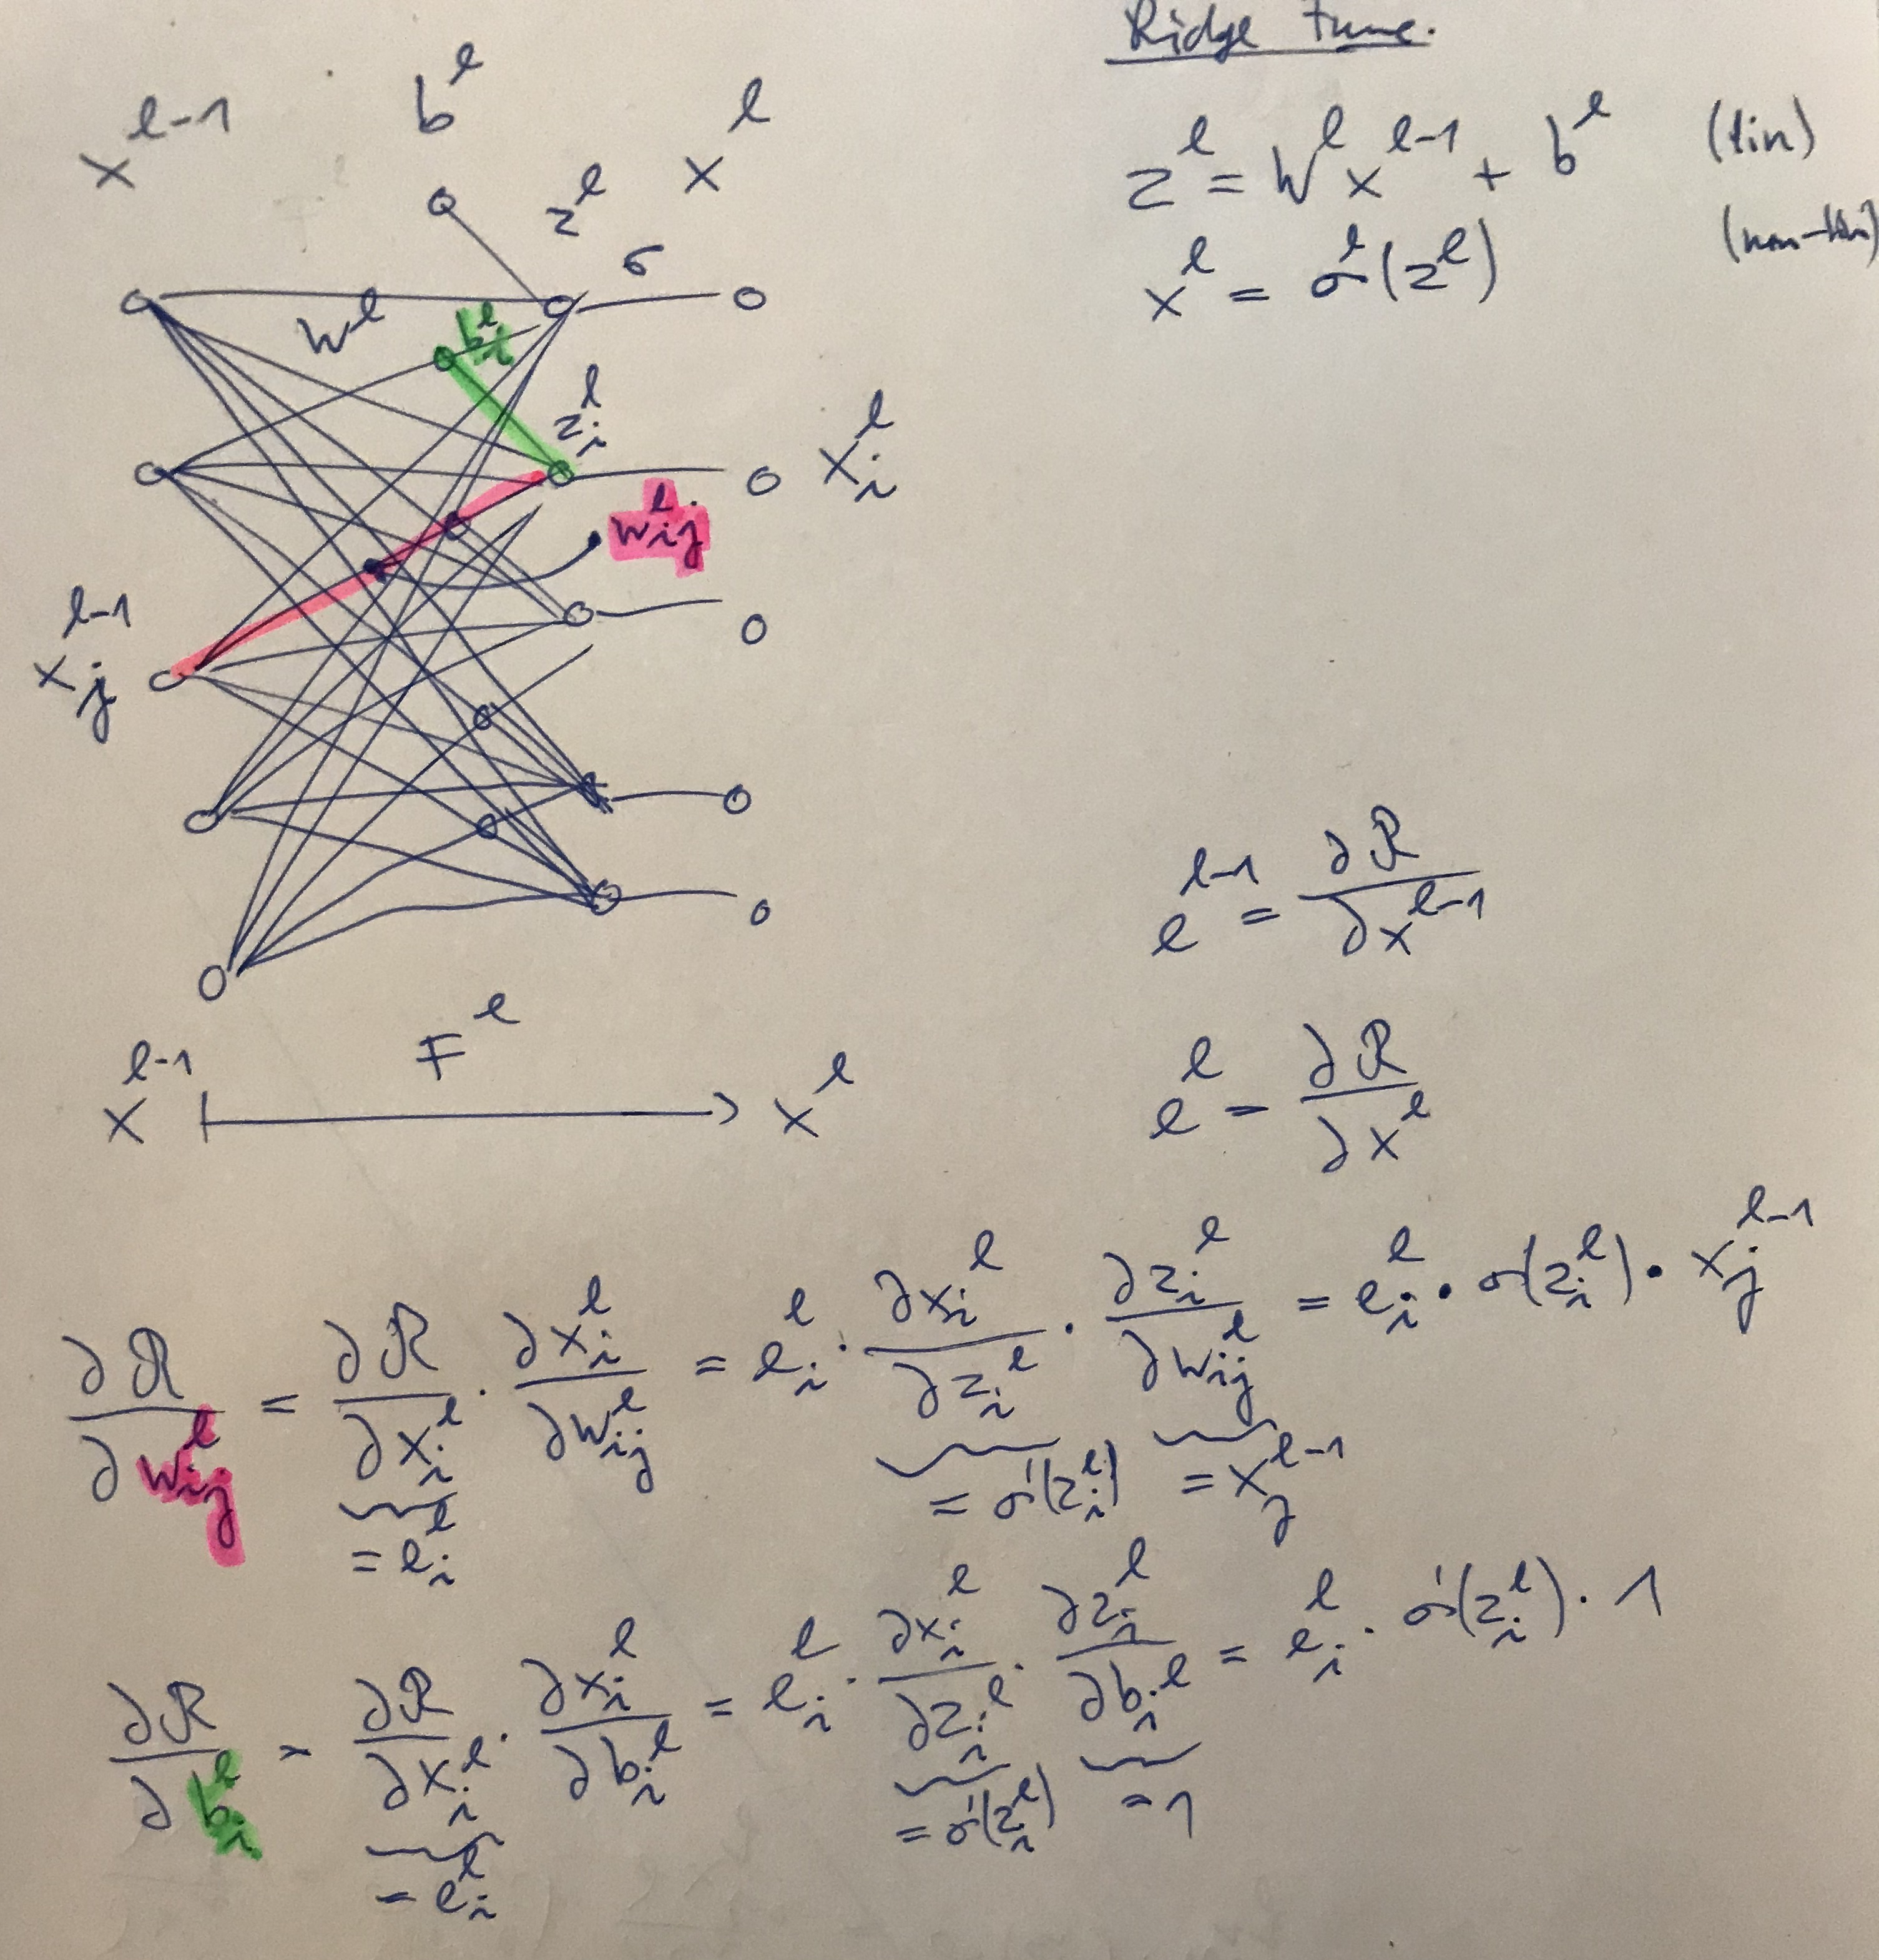
\includegraphics[width=1\linewidth]{%
%img/backprop-from-error-activations-to-parameter-gradients}
%\end{center}

$
\frac{\partial \cR}{\partial w_{ij}^l}
=
\underbrace{\frac{\partial \cR}{\partial x_i^l}}_{=e^l_i}
\frac{\partial x_i^l}{\partial w_{ij}^l}
=
e^l_i
\underbrace{\frac{\partial x_i^l}{\partial z_i^l}}_{=\sigma'(z_i^l)}
\underbrace{\frac{\partial z_i^l}{\partial w_{ij}^l}}_{=x_j^{l-1}}
=
e^l_i\sigma'(z_i^l)x_j^{l-1}
$

$
\frac{\partial \cR}{\partial b_i^l}
=
\underbrace{\frac{\partial \cR}{\partial x_i^l}}_{=e^l_i}
\frac{\partial x_i^l}{\partial b_i^l}
=
e^l_i
\underbrace{\frac{\partial x_i^l}{\partial z_i^l}}_{=\sigma'(z_i^l)}
\underbrace{\frac{\partial z_i^l}{\partial b_i^l}}_{=1}
=
e^l_i\sigma'(z_i^l).
$


%\frac{\partial }{\partial }


%\todo{Convert this to nice \LaTeX}

Note that in a way, the size of the gradient depends on the error that we have
times the strength of the network's output at some node.

%\sep

%\todo{Write the whole backpropagation algorithm. Or also the general
%backpropagation algorithm from the DL book.}


\subsection{Backpropagation Graphs}

The approach a backpropagation graph for a loss $L$ from a FF network graph is
as follows:
\begin{enumerate}
  \item (RED) Starting at the loss $L$ backward: for each node $n$ and for each
  of its outputs $o$ which has a path to the loss, add the node $\frac{\partial
  o}{\partial n}$ (at the height of node $n$). Connect the output $o$ and that
  node $n$ to that newly created node.
  \item (BROWN) Starting at the loss backward: for each node $n$ create a node
  $\frac{\partial L}{\partial n}$ (if it doesn't exist already) and connect each
  previously created partial node ($\frac{\partial o}{\partial n}$) to it, and
  the previously crated (in this step) $\frac{\partial L}{\partial o}$'s too.
\end{enumerate}

\begin{center}
  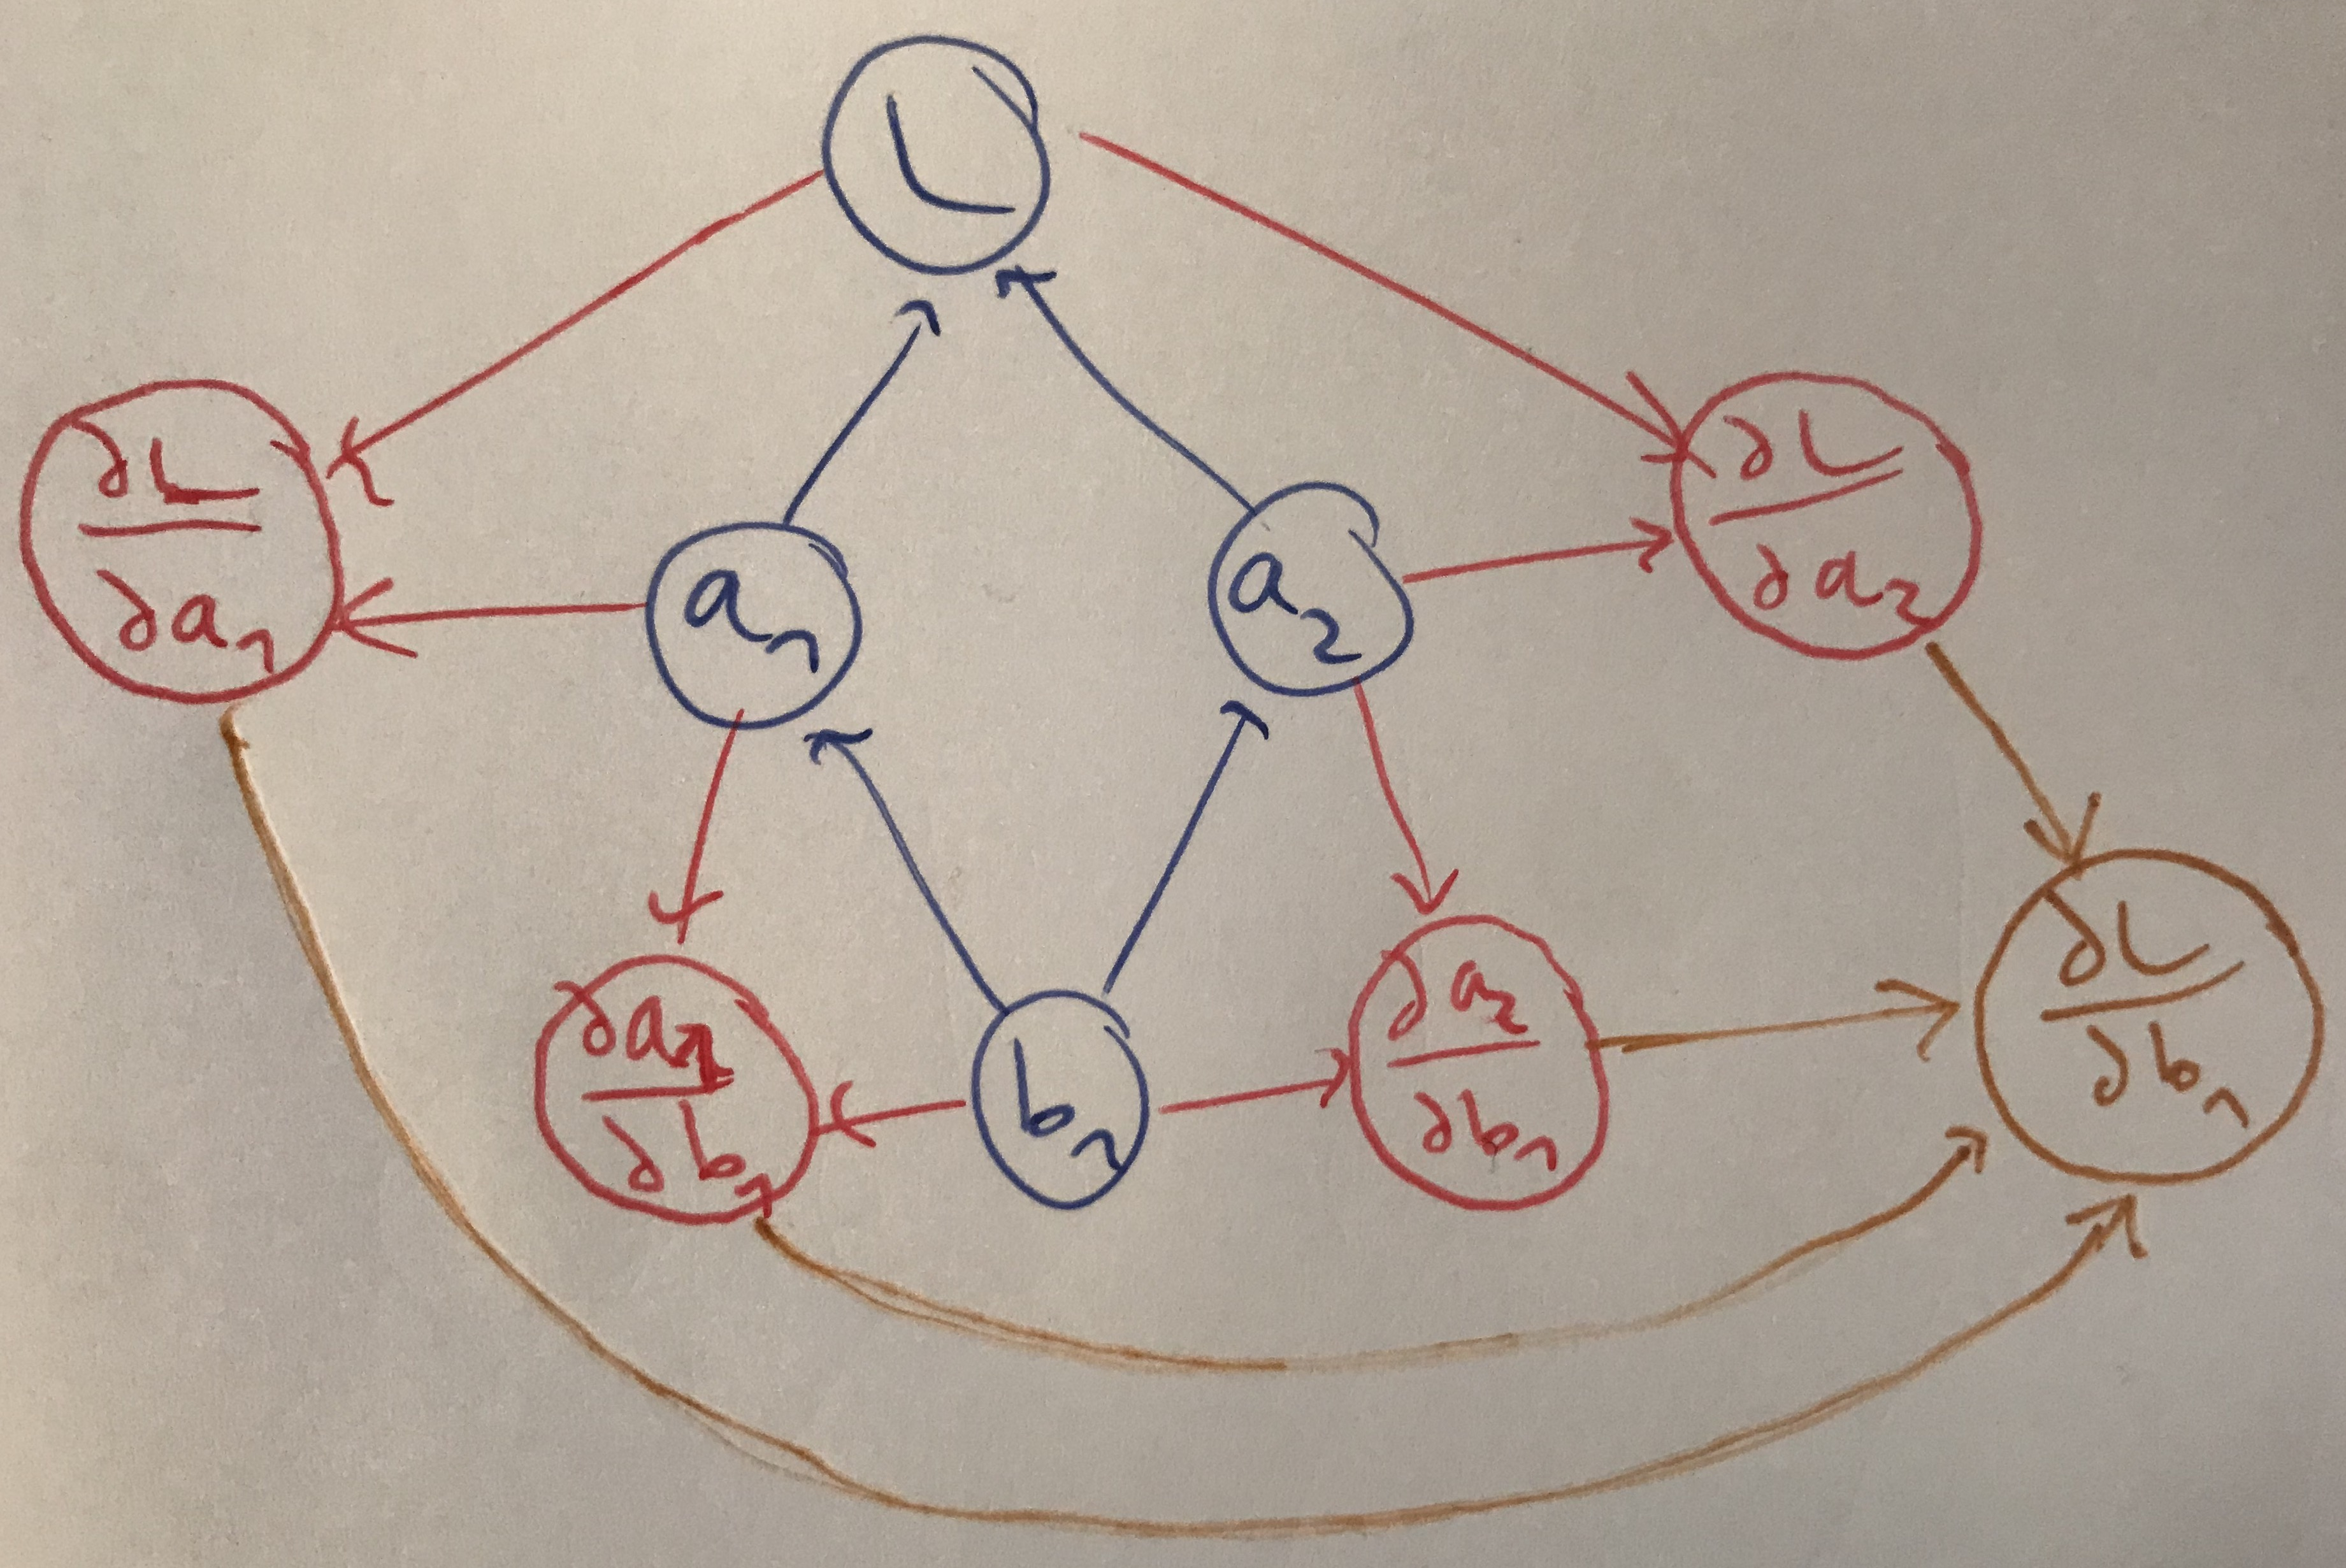
\includegraphics[width=0.7\linewidth]{%
img/backprop-graphs}
\end{center}

\section{Convolutional Neural Networks}

\subsection{Convolutional Layers}

\Def[Transform (aka Operator)] A transform $T$ is just a mapping from one
function space $\cF$ (or a cross product of it) to another function space $\cF'$. So
$T\colon\cF\to\cF'$.

\sep

\Def[Linear Transform (/Operator)] A transform $T$ is linear, if for all
functions $f,g$ and scalars $\alpha,\beta$, $T(\alpha f+\beta g)=\alpha (T f) +
\beta (T g)$.

\sep

\Def[Integral Transform (/Operator)] An \emph{integral transform} is
any transform $T$ of the following form

\[
(T f)(u)=
\int_{t_1}^{t_2} K(t,u) f(t) \, dt.
\]

The input of this transform is a function $f$ of $t$, and the output is another
function $Tf$ in terms of some other variable $u$.

Note that the integral boundaries, the class of input function $f$, and the
kernel $K$ must be defined such that $T f$ exists for any $f$ in order for $T$
to be an integral operator.

There are numerous useful integral transforms. Each is specified by a choice of
the function $K$ in two \emph{variables}, the \emph{kernel function},
\emph{integral kernel}, or \emph{nucleus} of the transform.

Some kernels have an associated \emph{inverse kernel} $K^{-1}(u,t)$, which
(roughly speaking) yields an inverse transform:

\[
f(t)=\int_{u_1}^{u_2} K^{-1}(u,t) (Tf)(u) \, du.
\]

\sep

\Thm Any integral transform is a linear transform.

\Cor The expectation operator is a linear operator.

\Proof Trivially follows from the linearity of the integral.

\sep

\Def[Symmetric Kernel]
A \emph{symmetric kernel} $K$ is one that is unchanged when the two variables
are \emph{permuted}. So, $K$ is symmetric, if $
K(t,u)=K(u,t).
$

\sep

Mathematical motivation: some problems are easier to solve if transformed and
solved in another domain (and then possibly the solution is transformed back).

DL motivation: we'll learn the kernels. 

\sep

\Def[Convolution] Given two functions $f, h\colon\R\to\R$, their convolution is
defined as

\[
(f * h)(u)
:=
\int_{-\infty}^{\infty}
h(t)f(u-t) \, dt
=
\int_{-\infty}^{\infty}
h(u-t)f(t)  \, dt
\]

\Com Whether the convolution exists depends on the properties of $f$ and $h$ (the
integral might diverge). However, a typical use is $f=\text{signal}$, and
$h=\text{fast decaying kernel function}$.

\sep

\Thm[Every Conv. can be Written as an Integral Transf.]

Now, a convolution of $f$ with some function $h$ can be seen as an
\emph{integral operator} with a kernel
\[
K(u,t) = h(u-t).
\]

Note that we can say the anologous thing for the convolution of $h$ with $f$.
The definition of the convolution shows us directly that it's
\emph{commutative}!

\ssep

\Lem The convolution $T(\argdot)=(\argdot \conv g)$ is a linear transform
(with $K(u,t)=g(u-t)$).

\Proof Trivially follows from the fact that we can express every convolution as
an integral transform.

\sep

\Thm[Convolution Properties]

\begin{itemize}
  \item Associativity $(f*g)*h=f*(g*h)$
  \item Commutativity $f*g=g*f$
  \item Bilinearity $(\alpha f+\beta g)\conv(\gamma y+\delta
  z)=\alpha\gamma(f\conv y)+\alpha\delta(f\conv z)+\cdots$\\
  (follows from commutativity and linearity)
\end{itemize}

\sep

\Def[Translation- (or Shift-) Invariant] A transform $T$ is translation (or
shift) invariant, if for any $f$ and scalar $\tau$,
\[
f_{\tau}(t):=f(t-\tau)\qquad(\text{Def. shift operator }s_{\tau})
\]
\[
(T f_{\tau})(t)
=
(T f)(t-\tau). \qquad\text{(commuting of operators holds)}
\]
So, an operator $T$ is shift-invariant iff it commutes with the shift operator
$s_\Delta$.
\[
\forall f\colon (T(s_{\Delta} f)) = (s_{\Delta}(T f)).
\]
So, the commutative diagram for this is:
\[
\begin{tikzcd}
f \arrow{r}{s_{\Delta}} 
\arrow[swap]{d}{T} 
& s_{\Delta} f = f_{\Delta}
\arrow{d}{T}
\\
T f
\arrow{r}{s_{\Delta}} 
& s_{\Delta}(T f) = T( f_{\Delta})
\end{tikzcd}
\]

\sep

\Thm[Convolution is Translation- (or Shift-) Invariant]

\Proof
$
\tau_{(s,t)} ((f\conv g)(u,v))
=(\tau_{(s,t)}(f)\conv g)(u,v)
=(f\conv\tau_{(s,t)}(g))(u,v)
$

\begin{align*}
\tau_{(s,t)} ((f\conv g)(u,v))
&=
\tau_{(s,t)}\left(\left(
\sum_{i=-p}^{p}
\sum_{j=-q}^q
f(u-i,v-j)g(i,j)
\right)(u,v)\right)
\\
&=
\sum_{i=-p}^{p}
\sum_{j=-q}^q
f(u+s-i,v+t-j)g(i,j)
\\
&=
\sum_{i=-p}^{p}
\sum_{j=-q}^q
\tau_{(s,t)}(f(u-i,v-j))g(i,j)
\\
&=
(\tau_{(s,t)}(f)\conv g)(u,v)
\end{align*}
\qed

\ssep

So, to summarize a \emph{convolution} is a \emph{linear
shift-invariant integral transform}.

\sep

\Thm[Convolution Theorem] Any linear, translation-invariant transformation $T$
can be written as a \emph{convolution} with a suitable $h$.

\ssep

\Proof

Let $\to$ represent the input-output relationship of a linear system.

By definition $\delta(t)\to h(t)$

Using linearity we have $a\delta(t)\to ah(t)$

Let $a=x(t')$ then $x(t')\delta(t)\to x(t')h(t)$

By shift invariance we have $\delta(t-t')\to h(t-t')$

Combining linearity and shift invariance $x(t')\delta(t-t')\to x(t')h(t-t')$

Again by linearity, we can sum many terms of this kind.

$
\int_{-\infty}^\infty x(t')\delta(t-t')\,dt'
\to 
\int_{-\infty}^\infty x(t')h(t-t')\,dt'
$

But by definition of $\delta(t)$ we have that the LHS is $x(t)$, so

$
x(t)
\to 
\int_{-\infty}^\infty x(t')h(t-t')\,dt'
$

By a change of variable on the RHS to $\tilde{t}=t-t'$ we also have

$
x(t)
\to 
\int_{-\infty}^\infty x(t-t')h(t')\,dt'
=y(t)
$
\qed

\subsection{Discrete Time Convolutions}

\Def[Discrete Convolution]

For $f,h\colon\Z\to\R$, we can define the discrete convolution via
\[
(f*h)[u]:=
\sum_{t=-\infty}^\infty
f[t]
h[u-t]
=
\sum_{t=-\infty}^\infty
f[u-t]
h[t]
\]

\Com Note that the use of rectangular brackets suggests that we're using
``arrays'' (discrete-time samples).

\Com Typically we use a $h$ with finite support (windows size).

\sep

\Def[Multidimensional Discrete Convolution] 

For $f,h\colon \R^d\to\R$ we have
\begin{gather*}
\begin{align*}
(f*h)[u_1,\ldots,u_d]
&=
\sum_{t_1=-\infty}^\infty
\cdots
\sum_{t_d=-\infty}^\infty
f(t_1,\ldots,t_d)
h(u_1-t_1,\ldots,u_d-t_d)
\\
&=
\sum_{t_1=-\infty}^\infty
\cdots
\sum_{t_d=-\infty}^\infty
f(u_1-t_1,\ldots,u_d-t_d)
h(t_1,\ldots,t_d)
\end{align*}
\end{gather*}

\sep

\Def[Discrete Cross-Correlation]

Let $f,h\colon\Z\to\R$, then
\begin{align*}
(h\star f)[u]
&:=
\sum_{t=-\infty}^\infty
h[t]f[u+t]
=
\sum_{t=-\infty}^\infty
h[-t]f[u-t]
\\
&=(\overline{h}*f)[u]
=(f*\overline{h})[u]
\qquad
\text{where }
\overline{h}(t)=h(-t).
\end{align*}

aka ``sliding inner product'', non-commutative, kernel ``flipped over'' ($u+t$
instead of $u-t$). If kernel symmetric: cross-correlation = convolution.

\subsection{Convolution via Matrices}

Represent the input signal, the kernel and the output as \emph{vectors}. Copy
the kernel as columns into the matrix ofsetting it by one more very time (gives
a band matrix (special case of Toeplitz matrix)). Then the convolution is just a
matrix-vector product.

\subsection{Why to use Convolutions in DL}

Transforms in NNs are usually: linear transform + nonlinearity. (given in
convolution).

Many signals obey translation invariance, so we'd like to have translation
invariant feature mpas. If the relationship of translation invariance is given
in the input-output relation then this is perfect.

\subsection{Border Handling}

There are different options to do this
\begin{itemize}
  \item \Def[Padding of $p$] Means we extend the image (or each dimension) by
  $p$ on both sides (so +2$p$) and just fill in a constant there (e.g., zero).
  \item \Def[Same Padding] our definition: padding with zeros = \emph{same
  padding} (``same'' constant, i.e., 0, and we'll get a tensor of the ``same'' dimensions)
  \item \Def[Valid Padding] only retain values from windows that are
  fully-contained within the support of the signal $f$ (see 2D example below) = \emph{valid padding}
\end{itemize}

\subsection{Backpropagation for Convolutions}

Exploits structural sparseness.

\sep

\Def[Receptive Field $\cI_i^l$ of $x_i^l$] 

The \emph{receptive field} $\cI_i^l$ of node $x_i^l$
is defined as
$
\cI_i^l
:=
\dset{j}{W^l_{ij}\neq 0}
$
where $\MW^l$ is the Toeplitz matrix of the convolution at layer $l$.

\Com Hence, the receptive field of a node $x_i^l$ are just nodes the which
are connected to it and have a non-zero weight.

\Com One may extend the definition of the receptive field over several layers.
The further we go back in layer, the bigger the receptive field becomes due to
the nested convolutions. The receptive field may be even the entire image
after a few layers. Hence, the convolutions have to be small.

\sep

Obviously, we have $
\forall j\neq \cI_i^l
\colon
\quad
\frac{\partial x_i^l}{\partial x_j^{l-1}}=0,
$ simply because
\begin{itemize}
  \item a node $x_j^{l-1}$ may not be connected to $x_i^l$,
  \item or a node $x_j^{l-1}$ may be connected to $x_i^l$ through an edge with zero
  weight, so $W_{ij}=0$ - hence, tweaking $x_j^{l-1}$ has no effect on
  $x_i^{l}$.
\end{itemize}

\sep

So due to the \emph{weight-sharing}, the kernel weight $h_j^l$ is re-used for
every unit in the target layer at layer $l$, so when computing the derivative
$\frac{\partial\cR}{\partial h_j^l}$ we just build an additive combination of
all the derivatives (note that some of them might be zero).
\[
\frac{\partial \cR}{\partial h_j^l}
=
\sum_{i=1}^{m_l}
\frac{\partial \cR}{\partial x_i^l}
\frac{\partial x_i^l}{\partial h_j^l}
\]

\sep

\textbf{Backpropagations of Convolutions as Convolutions}

$\vy^{(l)}$ output of $l$-th layer

$\vy^{(l-1)}$ output of $(l-1)$-th layer / input to $l$-th layer

$\vw$ convolution filter

$\frac{\partial\cR}{\partial \vy^{(l)}}$ known

$\vy^{(l+1)}=\vy^{(l)}\conv \vw$

\begin{align*}
\frac{\partial\cR}{\partial w_i}
&=\sum_{k}\frac{\partial\cR}{\partial y^{(l)}_k}\frac{\partial
y^{(l)}_k}{\partial w_i}
=\sum_{k}\frac{\partial\cR}{\partial y^{(l)}_k}\frac{\partial}{\partial w_i}
\left[\vy^{(l)}\conv\vw\right]_k
\\
&=\sum_{k}\frac{\partial\cR}{\partial y^{(l)}_k}\frac{\partial}{\partial w_i}
\left[\sum_{o=-p}^{p} y^{(l-1)}_{k-o}w_o\right]
=\sum_{k}\frac{\partial\cR}{\partial y^{(l)}_k}
y^{(l-1)}_{k-i}
\\
&=\sum_{k}\frac{\partial\cR}{\partial y^{(l)}_k}
y^{(l-1)}_{-(k-i)}
=\sum_{k}\frac{\partial\cR}{\partial y^{(l)}_k}
\text{rot180}(y^{(l-1)})_{k-i}
\\
&=\left(\frac{\partial\cR}{\partial \vy^{(l)}}
\conv\text{rot180}(y^{(l-1)})\right)_i
\end{align*}

The derivative $\frac{\partial\cR}{\partial\vy^{(l)}}$ is analogous.

Note that we just used generalized indices $i,k,o$ which may be
multi-dimensional.

This example omits activation functions and biases, but that could be easily
included with the chain-rule.

\sep

\Def[Rotation180] $\forall i\colon\text{rot180}(\vx)_i=\vx_{(-i)}.$

\subsection{Efficient Comp. of Convolutional Activities}

A naive way to compute the convolution of a signal of length $n$ and a kernel of
length $m$ gives an effort of $\BigO(m\cdot n)$. A faster way is to transform
both with the FFT and then just do element-wise multiplication (effort:
$\BigO(n\log n)$). However, this is rarely done in CNNs as the filters usually
are small ($m\ll n$, $m\approx \log(n)$).

\subsection{Typical Convolutional Layer Stages}

A typical setup of a convolutional layer is as follows:

\begin{enumerate}
  \item Convolution stage: affine transform
  \item Detector stage: nonlinearity (e.g., ReLU)
  \item Pooling stage: locally combine activities in some way (max, avg,
  \ldots)\\
  locality of the item that activated the neurons isn't too important, further
  we profit from dimensionality reduction. alternative: do convolution with
  stride. Another thing that turns out to be so is that most of the kernels that are
learned resemble a low-pass filter. Hence, when we sub-sample the images most of
the information is still contained.
\end{enumerate}

\subsection{Pooling}

The most frequently used pooling function is: \emph{max pooling}. But one
can imagine using other pooling functions, such as: min, avg, softmax,

\sep

\Def[Max-Pooling] 

Max pooling works, as follows, if we define a window size of $r=3$ (in 1D or
2D), then
\begin{itemize}
  \item 1D: $x_i^{\max}=\max \dset{x_{i+k}}{0\leq k < r}$
  \item 2D: $x_{ij}^{\max}=\max \dset{x_{i+k,j+l}}{0\leq k,l < r}$
\end{itemize}
So, in general we just take the maximum over a small ``patch''/''neighbourhood''
of some units.

\sep

\Thm[Max-Pooling: Invariance]

Let $\cT$ be the set of invertible transformations (e.g., integral transforms,
integal operators). Then $\cT$ forms a group w.r.t. function
composition: $\alg{\cT,\circ,{}^{-1},\id }$.

\todo{Understand what is meant on this slide!!!!}

\todo{Understand what is meant on this slide!!!!}

\todo{Understand what is meant on this slide!!!!}

\todo{Understand what is meant on this slide!!!!}

\todo{Understand what is meant on this slide!!!!}

\subsection{Sub-Sampling (aka ``Strides'')}

Often, it is desirable to reduce the size of the feature maps. That's why
sub-sampling was introduced.

\sep

\Def[Sub-Sampling] Hereby the temporal/spatial resolution is reduced.

\Com Often, the sub-sampling is done via a max-pooling according to some
interval step size (a.k.a. stride)

\sep

\begin{itemize}
  \con Loss of information
  \pro \todo{Depending on the transform we may get translation invariance???}
  \pro Dimensionality reduction
  \pro Increase of efficiency
\end{itemize}

\todo{Work out the backpropagation details for max-pooling}

\subsection{Channels}

\Ex Here we have
\begin{itemize}
  \item an input signal that is 2D with 3 channels (7x7x3) (image x channels)
  \item and we want to learn two filters $W0$ and $W1$, which each process the 3
  channels, and sum the results of the convolutions across each channel leading
  to a tensor of size 3x3x2 (convolution result x num convolutions)
\end{itemize}

\begin{center}
  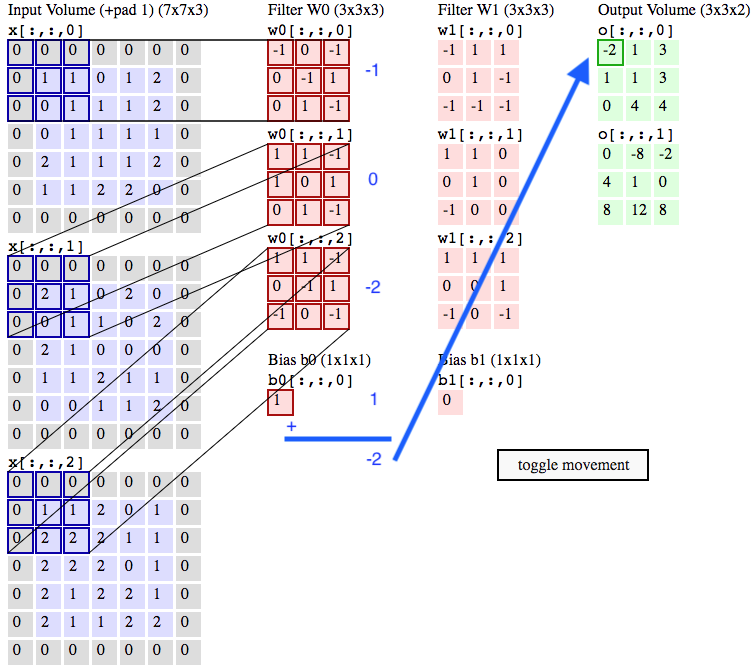
\includegraphics[width=0.5\linewidth]{%
img/convolutions-with-channels}
\end{center}

Usually we convolve over all of the channels together, such that each
convolution has the information of all channels at its disposition and the
order of the channels hence doesn't matter.

\subsection{CNNs in Computer Vision}

So the typical use of convolution that we have in vision is: a sequence of
convolutions
\begin{enumerate}
  \item that \emph{reduce} the spatial dimensions (sub-sampling), and
  \item that \emph{increase} the number of channels.
\end{enumerate}
The deeper we go in the network, we transform the spatial information into a
semantic representation. Usually, most of the parameters lie in the fully
connected layers

\subsection{Famous CNN Architectures}

\subsubsection{LeNet, 1989}

MNIST, 2 Convolutional Layers + 2 Fully-connected layers

\subsubsection{LeNet5}

MNIST, 3 Convolutional Layers (with max-pool subsampling) + 1 Fully connected
layer

\subsubsection{AlexNet}

ImageNet: similar to LeNet5, just deeper and using GPU (performance
breaktrhough)

\subsubsection{Inception Module}

Now, a problem that arose with this ever deeper and deeper channels were that
the filters at every layer were getting longer and longer and lots of their
coefficients were becoming zero (so no information flowing through). So, Arora
et al. came up with the idea of an inception module.

What this inception module does is just taking all the channels for one element
in the space, and reduces their dimensionality. Such that we don't get too deep
channels, and also compress the information (learning the low-dimensional
manifold).

This is what gave rise to the inception module:

\sep

\Def[Dimension Reduction] $m$ channels of a 1x1x$k$ convolution $m\leq k$:
\[
\vx^+{ij}=\sigma(\MW\vx_{ij}),\quad\MW\in\MR^{m\times k}.
\]
So it uses a 1x1 filter over the $k$ input channels (which is actually no
convolution), aka ``network within a network''.


\subsubsection{Google Inception Network}

The Google Inception Network uses many layers of this inception module along
with some other tricks
\begin{itemize}
  \item dimensionality reduction through the inception modules
  \item convolutions at various sizes, as different filter sizes turned out to
  be useful
  \item a max-pooling of the previous layer, and a dimensionality reduction of
  the result.
  \item 1x1 convs for dimension reduction before convolving with largerkernels
  \item then all these informations are passed to the next layer.
  \item gradient shortcuts: connect softmax layer at intermediate stages to have
  the gradient flow until the beginnings of the network.
  \item decomposition of convolution kernels for computational performance.
  \item all-in-all the dimensionality reductions improved the efficiency.
\end{itemize}

\subsection{Networks Similar to CNNs}

\Def[Locally Connected Network] A locally connected network has the same
connections that a CNN would have, however, the parameters are not shared. So
the output nodes do not connect to all nodes, just to a set of input nodes that
are considered ``near'' (locally connected).

\subsection{Comparison of \#Parameters (CNNs, FC, LC)}

\Ex input image $m\times n\times c$ ($c=$number of channels)

$K$ convolution kernels: $p\times q$  (valid padding and stride 1)

output dimensions: $(m-p+1)\times (n-q+1)\times K$

\ssep

\#parameters CNN: $K(pqc+1)$

\ssep

\#parameters of fully-conn. NN with same number of outputs as CNN:\\
$mnc((m-p+1)(n-q+1)+1)K$

\ssep

\#parameters of locally-conn. NN with same connections as CNN:\\
$pqc((m-p+1)(n-q+1)+1)K$

\sep

\Ex Assume we have an $m\times n$ image (with one channel).

And we convolve it with a filter $(2p+1)\times (2q+1)$

Then the convolved image has dimensions (assuming stride 1)
\begin{itemize}
  \item valid padding (only where it's defined): $(m-2p)\times (n-2q)$
  \item same padding (extend image with constant): $m\times n$ where the
  extended image has size $(m+2p)\times (n+2q)$.
\end{itemize}

\section{Optimization}

\subsection{Learning as Optimization}

Machine learning uses optimization, but it's \emph{not equal} to optimization
for two reasons:
\begin{enumerate}
  \item The empirical risk is only a \emph{proxy} for the expected risk
  \item The loss function may only be a \emph{surrogate}
\end{enumerate}

\subsection{Objectives as Expectations}

\[
\nabla_{\theta}\cR(D)
=
\Exp[\cS_N\sim p_D]{\nabla_{\theta}\cR(\cS_N)}
=
\Exp{
\frac{1}{N}
\sum_{i=1}^N
\nabla_{\theta}\cR(\theta;\set{\vx[i],\vy[i]})
}
\]

The typical structure of a learning objective in a NN is a \emph{large finite
sum} (over all training instances). Accuracy-complexity trade-off: in practice
we subsample terms in the sum, by using \emph{mini-batches} of the training data 
(so we'll get something close to the true gradient - but not exactly). The idea
behind it, is that everything will work out in expectation. Further, we favour
cheap and imprecise computations over many datapoints rather than precise and
expensive computations over a few datapoints.

\subsection{Gradient Descent}

$
\theta(t+1)=\theta(t)-\eta_t\nabla_\theta\cR,
$

$
\dot{\theta}=-\eta_t\nabla_\theta\cR(\theta)
$

\todo{Mention how line search works: Euler Method. Search for the optimal
$\eta$ in the direction of the gradient such that we get to a minimum, so
$\argmin_\eta$}

\subsection{Gradient Descent: Classic Analysis}

In classical machine learning we have a \tcg{\emph{convex}} objective $\cR$. And
we denote
\begin{itemize}
  \item $\cR^*$ as the minimum of $\cR$
  \item $\theta^*$ as the optimal set of parameters (the minimizer of $\cR$)
\end{itemize}
So we have
$
\forall\theta\neq\theta^*\colon\cR^*:=\cR(\theta^*)\leq\cR(\theta).
$

\sep

\Def[Strictly Convex Objective] $\to$ objective has only one (a unique)
minimum.
\[
\forall\theta\neq\theta^*\colon\cR^*:=\cR(\theta^*)\mcg{<}\cR(\theta).
\]

\sep

\Def[$L$-Lipschitz Continous Function] Given two \emph{metric spaces} $(X, d_X)$
and $(Y, d_Y)$, where $d_X$ denotes the \emph{metric} on the set $X$, and $d_Y$
denotes the metric on set $Y$, a function $f\colon X\to Y$ is called
\emph{Lipschitz continuous}, if there exists a real constant $L\in\R^+_0$, such
that
\[
\forall x_1,x_2\in X
\colon\quad
d_Y(f(x_1),f(x_2))
\leq
L\cdot
d_X(x_1,x_2).
\]
Hereby, $L$ is referred to as a \emph{Lipschitz constant} for $f$.
\begin{itemize}
  \item If $L=1$ the function is called a \emph{short map}
  \item If $0\leq L < 1	$ and $f$ maps a metric space to itself, so $f\colon X
  \to X$, then the function $f$ is called a \emph{contraction}.
\end{itemize}

In particular, a map $f\colon\R^n\to\R^m$ is called Lipschitz continous if
there exists a $L\in\R^+_0$ such that

\[
\forall\vx_1,\vx_2\in\R^n
\colon\quad
\underbrace{\norm{f(\vx_1) - f(\vx_2)}}_{=d_{\R^m}(f(\vx_1),f(\vx_2))}
\leq
L\cdot
\underbrace{\norm{\vx_1-\vx_2}}_{d_{\R^n}(\vx_1,\vx_2)}.
\]

\ssep

\Ex So for our risk function $\cR$, we say that the gradient of it
\[
\nabla_\theta\cR\colon\Omega\to\Omega
\quad
\text{where }\Omega=\R^n
\]
is $L$-Lipschitz continous, if it holds that
\[
\forall\theta_1,\theta_2\in\Theta
\colon\quad
\norm{\nabla_\theta\cR(\theta_1)-\nabla_\theta\cR(\theta_2)}
\leq
L\norm{\theta_1-\theta_2}
\]

\Com So, the $L$ tells us how big the gradient could be.

\sep

\Thm We have the following chain of inclusions for functions over a
\emph{closed} and \emph{bounded} (i.e., compact) subset of the real line.

Continously differentiable $\subseteq$ Lipschitz continuous $\subseteq$
(Uniformly) continous

\Com It's important that the space is bounded. Because for example only on a
compact subset $[a,b]\subset\R$ the function $e^x$ is Lipschitz continous. On
$\R$ the function $e^x$ is not Lipschitz continuous, as it gets arbitrarily
steep.

\todo{Does this also hold for compact vector-spaces?}

\todo{Add Properties listed on Wikipedia! Very useful for understanding!}

\url{https://en.wikipedia.org/wiki/Lipschitz_continuity#Properties}

\sep

\Thm An everywhere differentiable function $f\colon\R\to\R$ is Lipschitz
continuous (with $L=\sup\abs{f'(x)}$) iff it has \emph{bounded first
derivatives}.

\ssep

\Thm In particular any continously differentiable function is \emph{locally}
Lipschitz continuous. As continuous functions are bounded on an interval, so its
gradient is locally bounded as well.

\sep

\Thm If $\cR$ is convex with $L$-Lipschitz-continuous gradients then
we have that 
\[ 
\cR(\theta(t))-\cR^* \leq
\frac{2L}{t+1}
\norm{\theta(0)-\theta^*}^2 \in\BigO(t^{-1}) 
\] 
\Com So we have a polynomial (linear) convergence rate of $\theta$ towards the
optimal parameter $\theta^*$ (note: just in the convex setting!). As we can see,
the convergence time is bounded by a time that depends on our initial guess, and
the Lipschitz constant $L$.

\Com Usually one value for $\eta$ that people use in this setting is
$\eta:=\frac{1}{L}$ or $\eta:=\frac{2}{L}$.

\Proof See 
\href{https://perso.telecom-paristech.fr/rgower/%
pdf/M2_statistique_optimisation/grad_conv.pdf}{here}

\sep

\Def[Convex Set] A set $S\subseteq\R^d$ is called \emph{convex} if

$
\forall\vx,\vx'\in\S, \,\,\forall\lambda\in[0,1]\colon\quad
\lambda\vx+(1-\lambda)\vx'\in S.
$

\Com Any point on the line between two points is within the set.

\sep

\Def[Convex Function] A function $f\colon S\to\R$ defined on a \emph{convex set}
$S\subseteq\R^d$ is called \emph{convex} if
\[
\forall\vx,\vx'\in S, \,\lambda\in[0,1]\colon\quad
f(\lambda\vx + (1-\lambda)\vx')
\leq
\lambda f(\vx) + (1-\lambda)f(\vx)  
\]

\Com convex combination of two points $<$ evaluation of convex combination of
two points.

\Com Another way to formulate that $f$ is convex function is to say that the
epi-graph of $f$ is a convex set.

\sep

\Thm Every local optimum of a convex function is a global optimum.

\sep

\Thm[Operations that Preserve Convexity]
\begin{itemize}
  \item $-f$ is concave if and only if $f$ is convex
  \item nonnegative weighted sums
  \item point/element-wise maximum $\max(f_1(\vx),\ldots,f_n(\vx))$
  \item composition with non-decreasing function, e.g. $e^{f(\vx)}$
  \item composition with affine mapping: $f(\MA\vx+\vb)$
  \item restriction to a line (of convex set domain)
\end{itemize}

\sep

\Def[Strictly Convex Function] $f$ is called \emph{strictly convex} if
\[
\forall\vx,\vx'\in S,\vx\neq\vx' \,\lambda\in[0,1]\colon\quad
f(\lambda\vx + (1-\lambda)\vx')
<
\lambda f(\vx) + (1-\lambda)f(\vx)  
\]
\sep

\Def[Strongly Convex Function] A differentiable function $f$ is called
\emph{$\mu$-strongly convex} if the following inequality holds for all points
$\vx,\vy$ in its domain:
\[
\forall\vx\vy\colon\quad
\scprod{\nabla f(\vy)-\nabla f(\vx),\vy-\vx}
\geq
\mu\norm{\vy-\vx}_2^2
\]
where $\norm{\argdot}$ is any norm. An equivalent condition is the following:
\[
\forall\vx,\vy\colon\quad
f(\vy)\geq f(\vx)
+\nabla f(\vx)^\T(\vy-\vx) + \frac{\mu}{2}\norm{\vy-\vx}_2^2.
\]

\ssep

\Com 
The concept of strong convexity extends and parametrizes the notion of strict
convexity. A strongly convex function is also strictly convex, but not vice
versa. Notice how the definition of strong convexity approaches the definition
for strict convexity as $\mu\to 0$, and is identical to the definition of a
convex function when $\mu=0$. Despite this, functions exist that are strictly
convex, but are not strongly convex for any $\mu>0$.

\todo{Add an illustration how $\mu$-strong convexity allows not to only place a
tangent below the graph at any point on the graph, but actually a parabola, so
the function is acutally even more curved (controlled by $\mu$).}

%\todo{Visit other useful hints about strong convexity!!!!!!}

%\href{%
%https://en.wikipedia.org/wiki/Convex_function#Strongly_convex_functions
%}{<<Strong Convexity Link>>}

\sep

\Thm Now, when $\cR$ is $\mu$-strongly convex in $\theta$ and its gradient is
$L$-Lipschitz continuous $\Longrightarrow$
\[
\cR(\theta(t))
-
\cR^*
\leq
\left(1-\frac{\mu}{L}\right)^t
(\cR(\theta(0))-\cR^*)
\in
\BigO\left(\left(1-\frac{\mu}{L}\right)^t\right)
\]

So we have
\begin{itemize}
  \item an exponential convergence (``linear rate'')
  \item and the rate depends adversely on the condition number $\frac{L}{\mu}$.
  So we want the maximum gradient to be small, and we want the curvature to be
  large (which are somewhat contrary desires, but ideally the condition number
  is very close to $1$).
\end{itemize}

\sep

\Thm If we use Nesterov acceleration (in the general case), then we get a
polynomial convergence rate of $\BigO(t^{-2})$.

\Com The trick used in the Nesterov approach is \emph{momentum}.

\todo{What is meant by \emph{general case}?}

\subsection{Optimization Challenges in NNs: Curvatures}

When it comes to NNs the objective is usually non-convex. So this is for example
an objective that we may get that is non-convex. Still, we can apply gradient
descent in this setting. And if we respect the rule of choosing the learning
rate as $\eta=\frac{1}{L}$ where $L$ is the Lipschitz-constant of the function,
then usually, we're fine.

\begin{center}
  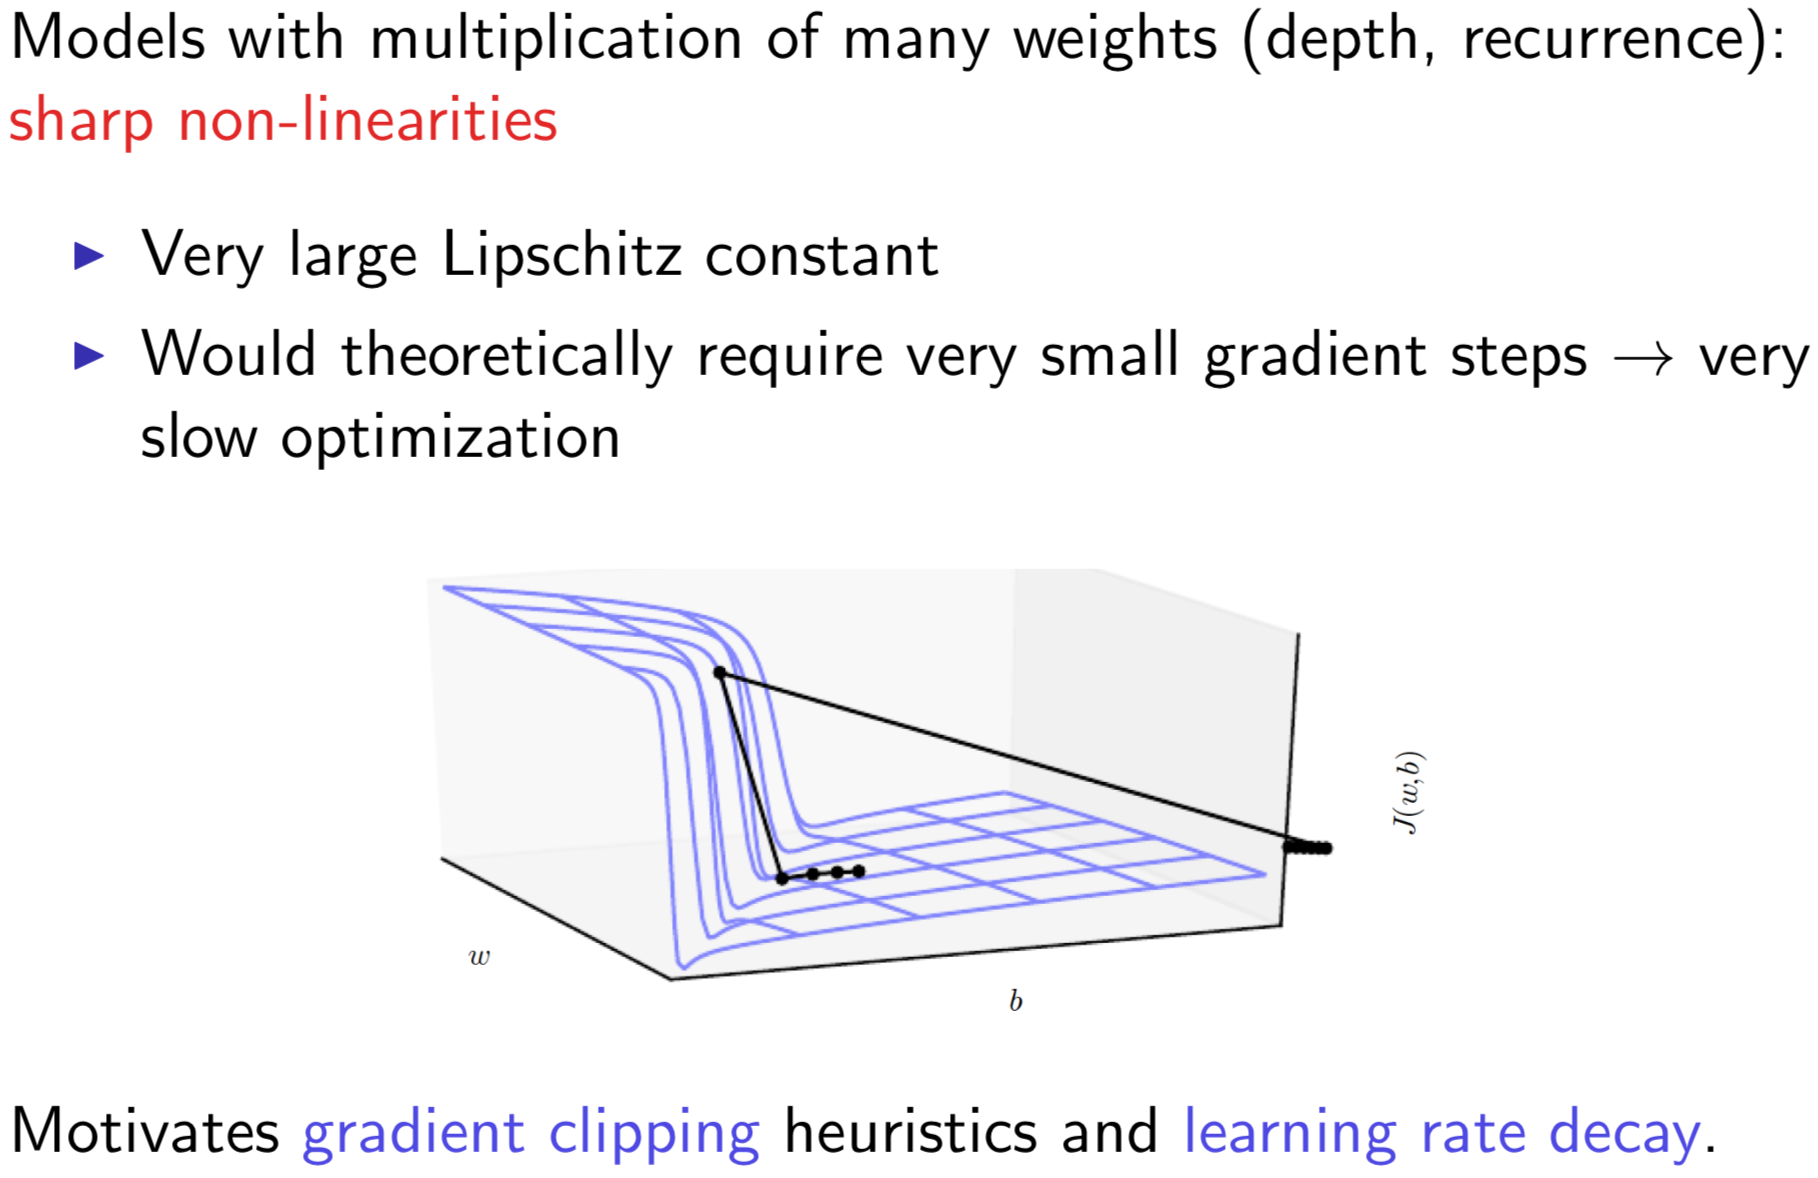
\includegraphics[width=1\linewidth]{%
img/challenge-curvature}
\end{center}

So the problem is if we have sharp non-linearities, then there are two
approaches to solve this
\begin{itemize}
  \item one is to be very conservative and only do small update steps by
  choosing a very small learning rate.
  \item or we are courageous and due huge jumps as depicted in the image.
\end{itemize}
So this is kindof the typical problem that, at least some people think, happens
with NNs.

Typical approaches are to clip the gradient when it gets too large, or use a
decreasing learning rate (in terms of time).

Now, the problem is not that the cliff is very steep. The problem is the
curvature. Because when we take the gradient, the gradient is actually constant
on the wall of the cliff. Let's have a look at this through some equations.

Now, let's evaluate what the risk is at some point, plus some gradient step. If
we do the 2nd-order Taylor expansion of that, then we get
\[
\cR(\theta-\eta\nabla_{\theta}\cR(\theta))
\stackrel{\text{Taylor}}{\approx}
\cR(\theta)
-\eta\norm{\nabla_\theta\cR(\theta)}_2^2
+
\frac{\eta^2}{2}
\underbrace{
\nabla_{\theta}\cR(\theta)^\T\MH
\nabla_{\theta}\cR(\theta)
}_{\norm{\nabla_\theta\cR(\theta)}_{\MH}^2}
\]
where
\[
\MH:=\nabla^2\cR(\theta)
\qquad
\text{(Hessian matrix)}
\]
\todo{Shouldn't $\MH$ be denoted as an inverse somewhere?} 

Now, what we want is that the rest of the sum \todo{which?} is negative. If that
is the case, because then we're improving our cost function. If not, then we're
basically diverging. \todo{understand argument}

So,
\begin{itemize}
  \item the first term $-\eta\norm{\nabla_\theta\cR(\theta)}_2^2$ will obviously
  be negative, as it's a negative factor of a norm
  \item the second term will always be positive, as the hessian matrix is
  positive semi-definite. Fortunately, we're squaring $\eta$, which may be
  already small, so the term is small. However, if the Hessian is
  ill-conditioned (as in the cliff-situation (curvature)). Then we can have a
  very large positive value in the second term. So what then can happen is that
  \[
  \frac{\eta}{2}\norm{\nabla_\theta\cR(\theta)}_{\MH}^2
  \gtrsim
  \norm{\nabla_\theta\cR(\theta)}^2
  \]
  So, the hessian term becomes much larger than the gradient. So we're not
  improving our cost function.
  \todo{Shouldn't there be a square on $\eta$? What does this symbol mean?}
  \item and the remaining terms, will be negative (as defined by the Taylor sum)
\end{itemize}

So a typical remedy for first-order methods is to take very small step sizes
$\eta$.

\sep

However, things bececome even stranger because of the curvature. As we can see,
the gradient norm gets larger and larger the more we train (can be checked
empirically). And the gradient norm also tends to have larger fluctuations. And
as we can see, starting at some point, the error just fluctuates around at a
certain level. Actually, one might assume that as we're getting closer to the
minimum, the gradient should get smaller and smaller, as the objective gets
flatter and flatter at the optimal point - but that's actually not the case!

\begin{center}
  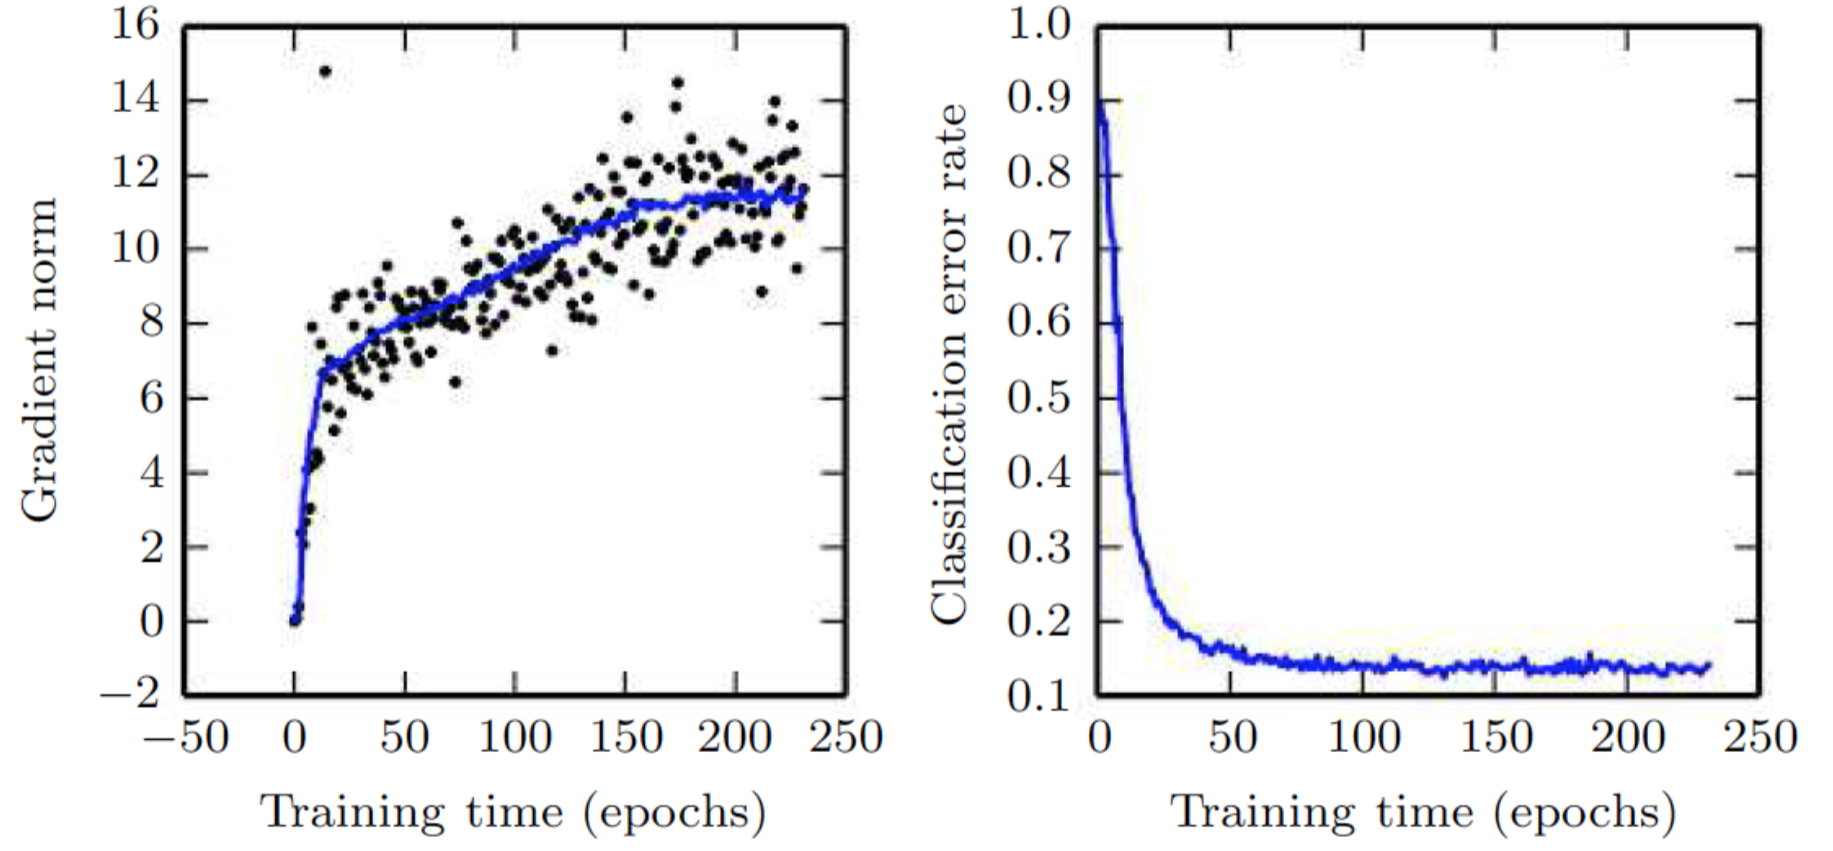
\includegraphics[width=1\linewidth]{%
img/challenges-curvature-and-gradients}
\end{center}

This is probably so, because we're dealing with large curvatures when reaching
(or getting close to) the optimal parameters. So with gradient descent we may
not arrive at a critical point of any kind, and this also motivates to use more
and more decreasing learning rates, the closer we get to the optimal parameters.
Note that this graph was built using the MNIST dataset and some CNN.

Note that there exist many architectures where the final gradient was very
large, and still they are used in practice, and people are quite happy with
them.

\subsection{Optimization Challenges in NNs: Local Minima}

At the beginning people were happy when they were doing convex optimization
because there was a single optimum and it was reachable. And then when people
started using non-convex optimization they were afraid of getting into
non-optimal local minima and getting stuck there.

\ssep

Neural network cost functions can have many local minima and/or saddle points -
and this is typical. Gradient descent can get stuck.

Questions that have been looked at are
\begin{itemize}
  \item Ar local minima a practical issue? Somtimes not: Gori \& Tesi, 1992
  \item Do local minima even exist? Sometimes not (auto encoder): Baldi \&
  Hornik, 1989
  \item Are local minima typically worse? often not (large networks): e.g.,
  Choromanska et al, 2015
  \item Can we understand the learning dynamics? Deep linear case has
  similarities with non-linear case, e.g., Saxe et al., 2013
\end{itemize}

So it turns out that the non-convexity is actually not so much of an issue. It
turns out that when we go to very high dimensions, the number of local minima VS
the number of saddle points (gradient is zero, but non-optimal) is very small -
so we're much more likely to end up in a saddle point. However, in practice, if
we do SGD there is some stochasticity that will make our gradient move. Then,
after waiting for a while we'll exit the saddle point.


\Def[Epoch = one sweep through the whole data]
\begin{itemize}
  \item take the data batch by batch
  \item compute one gradient by batch
  \item harder to analyze theoretically
  \item typically works better in practice
  \item no permutation $\to$ danger of ``unlearning''. Let's suppose we're
  training for MNIST, and we're first doing the gradient steps for the 1s, then
  for the 2s, etc. This will completely bias the gradient and lead us into the
  wrong direction at every gradient step. In the end we'll never converge to a
  good solution.
\end{itemize}

\Com It happens that this way SGD is a bit harder to analyze theoretically, but
for NNs it works quite well in practice.

\ssep

\Def[Minibatch Size]
\begin{itemize}
  \item ``Standard SGD'': $k=1$, this is for classical SGD. 
  However, if we only take one instance, the error on the gradient 
  direction will be too large.
  \item but: larger $k$ is better for utilizing concurrency in GPUs or multicore
  CPUs. And we'll also get more accuracy. Of course, this requires more
  computation per gradient step, so we'll have to compute more to do one step,
  but it pays of in terms of accuracy of the gradient (and it can be
  parallelized anyways).
\end{itemize}

\Com In practice we just need to ensure that the batch is sufficiently big to
have a representative subsample to compute a reliable estimate of the gradient
(in order to converge). Further, we usually use batch-sizes of $2^k$ for some
$k\in\N$.

\subsubsection{Convergence Rates}

Under certain conditions SGD converges to the optimum:
\begin{itemize}
  \item If we have a convex, or strongly convex objective,
  \item and if we have Lipschitz continous gradients,
  \item and a deaying learning rate, s.t.
  \[
  \underbrace{\sum_{t=1}^\infty\eta_t=\infty}_{\mathclap{\text{we get far
  enough}}},
  \qquad
  \underbrace{\sum_{t=1}^\infty\eta_t^2<\infty}_{\text{our steps get always
  smaller}}
  \]
  typically $\eta_t=Ct^{-\alpha}$, $\frac{1}{2}<\alpha<1$ (c.f. harmonic
  series.)
  \item or we use iterate (Polyak) averaging (once we start jumping around, we
  average the solutions over time).
\end{itemize}
Then, we can get the following convergence rates:
\begin{itemize}
  \item strongly-convex case: can achieve a $\BigO(1/t)$ suboptimality rate
  (only polynomial convergence)
  \item non-strongly convex case: $\BigO(1/\sqrt{t})$ suboptimality rate (even
  worse than polynomial convergence)
\end{itemize}
So, even if the convergence rates are not super nice, thanks to the cheap
gradient computation (only one example at the time), we may even converge faster
than computing the gradient on the full dataset everytime.

\subsubsection{Practicalities}

Now, let's have a look at some of the practicalities:
\begin{itemize}
  \item Almost none of the analysis applies to the non-convex case
  \item Choosing a learning rate schedule can be a nuisance
  \item Fast decay schedules may lead to super-slow convergence
  \item In practice, we tend to use larger step sizes and level out at a minimal
  step size. The justification behind this that the SGD with a fixed step size
  is known to converge to a ball around the optimum (strongly convex case). So
  we may use
  \[
  \eta_t=\max(0.001,\frac{1}{t}).
  \]
  \item Further, there's the common belief that the stochasticity of the SGD is
  a ``feature'', since it may help to escape from reagions with small gradients
  via perturbations.
\end{itemize}

\subsubsection{Momentum}

Accumulate the gradient over several updates (as a geometrically weighted
average). The momentum (averaging) keeps the gradient moving better towards the
optimum (instead of zig-zagging).

Initialization: $\alpha=0.95$ (typically), $\vm(0)=\vo$.

Then at every timestep $t=1,2,\ldots$

$
\vm(t)=\alpha \vm(t-1)-(1-\alpha)\nabla_\theta\cR(\vtheta(t-1)),
$

$
\vhm(t)=\frac{\vm(t)}{(1-\alpha)^t}
$ \quad(bias correction, otw. gradient is too small at beginning)

$
\vtheta(t)=\vtheta(t-1)-\eta\vhm(t)
$ \quad (update parameters)

Usually it's good to choose a small alpha (0.5) at the beginning, and only
towards the end, we'll increase alpha to 0.99 to accumulate and average the
speed.

\subsubsection{Nesterov Momentum}

First jump, and then compute the momentum based on the gradient at the place
that we'll land (seems to work better in practice).

$
\vtheta(t+1)=\vtheta(t)+\eta\alpha\vhm(t)
$ (jump first)

$
\vv(t+1)=\alpha \vv(t) +
\epsilon\nabla_\theta\cR(\vtheta(t)+\alpha\vhm(t)).
$ (and then correct the jump with the gradient at the place that we jumped to)

\todo{Write this down correctly!}

\subsubsection{AdaGrad}

With AdaGrad we consider the entire history of gradients and put all the
gradients ito a \emph{gradient matrix}, so
\[
\theta\in\R^d,
\quad
\MG\in\R^{d\times t_{\max}},
\quad
g_{it}
=
\evalat{\frac{\partial \cR(t)}{\partial \theta_i}}{\theta=\theta(t)}
\]
Then we compute the (partial) row sums of squares of $\MG$ (note: not the
gradient norms! $\to$ rows!)
\[
\gamma_i^2(t):=\sum_{s=1}^tg_{is}^2.
\]
And then we adapt the gradient stepsize for each dimension as follows:
\[
\theta_i(t+1)=\theta_i(t)-\frac{\eta}{\delta+\gamma_i(t)}\nabla_\theta\cR(t),
\qquad
\delta>0\text{ (small)}
\]
This will transform the gradient such as if the loss landscape would be in a
more isometric shape. It will scale the gradient appropriately into each
dimension. So instead of having a valley, we'll have a nice round hole again.
This avoids this typical situation where the gradient descent boundes left and
right in the valley, instead of walking down the valley.

\sep

\todo{maybe take notes from Data Mining}

\sep

In practice a variant of AdaGrad (RMSprop) is used. Intuitively: the learning
rate decays faster for weights that have seen significant updates.

Theoretical justification: regret bounds for convex objectives (Duchi, Hazan,
Singer, 2011) (out of scope for this lecture).

So, Tieleman \& Hinton came up with a ``non-convex variant of AdaGrad'' in 2012:
\[
\gamma_i^2(t):=\sum_{s=1}^t\rho^{t-s}g_{is}^2,
\qquad
\rho<1.
\]
This is just a moving average, which is exponentially weighted. The weight
decays exponentially over time, and thus \todo{give explanation}.

It turns out that this optimizer works very nice some times.

\subsubsection{ADAM}

Adam is probably the most popular optimizer today. It takes the best of both
worlds: AdaGrad (adapting the gradient) + Momentum. However, more parameters to
tune $(\beta_1,\beta_2)$.

Initialization: $\vm(0)=\vo$, $\vv(0)=\vo$

Typical values: $\beta_1=0.9$, $\beta_2=0.999$, $\epsilon=10^{-8}$

Then at every timestep $t=1,2,\ldots$

$\vg(t)=\nabla_{\theta}\cR(\vtheta(t-1))$ (get the gradient)

$\vm(t)=\beta_1 \vm(t-1)+(1-\beta_1)\vg(t)$ (update the biased first moment
estimate)

$\vv(t)=\beta_2 \vv(t-1)+(1-\beta_2)\vg(t)^2$ (update the b. second raw moment
estimate)

$\hat{\vm}(t)=\vm(t)(1-\beta_1^t)$ (bias correction first moment estimate)

$\hat{\vv}(t)=\vv(t)(1-\beta_2^t)$ (bias correction second raw moment estimate)

$\vtheta(t)=\vtheta(t-1)+\eta\hat{\vm}(t)/(\sqrt{\hat{\vv}(t)}+\epsilon)$
(update params)

\subsection{Optimization Heuristics}

\todo{What did we want to do with this section???}

Polyak Averaging may bring us good guarantees if we have a convex loss (on
average). However, for DL it's not ideal. The reason are
\begin{itemize}
  \item if we may want to have an idea over what the gradient over the whole
  dataset would be, then we'd have to swipe over all the dataset which will take
  a lot of time. So, it's nood a good idea (we'll get a better but slower
  convergence). So what people do in practice instead is that they just run a
  weighted average to forget what was in the past. Usually, the weighted  
  \item 
\end{itemize} 

\subsubsection{Batch Normalization}

Batch normalization (Ioffe \& Szegedy, 2015) is one of the most controversial
but most useful tricks in DL. 

One of the big problems that we have when we optimize NNs, is that usually there
exist strong dependencies between the weights in various layers (recall: we also
saw that the gradients interact with each other through complex dynamics). So
it's hard to find a suitable learning rate for all the situations of the
weights. The dynamics were fine in this case, but if we have a large network it
might not work out, and we may have to wait a long time until the dynamics
diminish and lead to the solution. What batch normalization tries to achieve is
to remove the dependencies between the layers. So the learning algorithm can
optimize the weights of each layer independently. Of course, that's not really
what happens, but anyways that's the idea behind it.

\ssep

The key idea of batch-normalization is to normalize the layer activations
($\to$ batch normalization) and then to backpropagate through the normalization.
So it ``keeps the same distribution'' at each layer. And if we optimize the
weights of a layer, it should not affect the distribution at the end of the
layer.

So what we do is
\begin{itemize}
  \item we fix a layer $l$,
  \item and we fix a set of examples $I\subset[1:N]$
  \item and compute the mean activities and a vector of the standard deviations
\begin{align*}
\vmu^{l}
&:=
\frac{1}{\card{I}}
\sum_{i\in I}
(F^l\circ\cdots\circ F^1)(\vx[i])\in\R^{m_l}
\\
\vsigma^l&\in\R^{m_l}
\\
\sigma_j^l
&:=
\sqrt{
\delta
+
\frac{1}{\card{I}}
\sum_{i\in I}
\left(
(F^l_j\circ\cdots\circ F^1)(\vx[i])
-\mu_j^l
\right)^2
},
\quad
\delta > 0,
\end{align*}
  \item then we remove the mean and divide by the standard deviation to
  normalize the activities.
  \[
  \tilde{x}_j^l
  :=\frac{x_j^l-\mu_j^l}{\sigma_j^l}
  \]
  However, when we do this, what happens is that we can represent less than
  before. We may only have distributions with mean zero, and variance one
  (because we enforce this through the normalization). So we need to do
  something to regain the representational power. What we do is we multiply by
  some coefficients $\alpha_j$ and $\beta_j$
  \[
  \tilde{\tilde{x}}_j^l=\alpha_j^l\tilde{x}_j^l+\beta_j^l
  \]
\end{itemize}
So since $\vmu$ and $\vsigma$ are functions of the weights and they can be
differentiated. 

\todo{Write down gradients of batch-norm layer}

\todo{Write down gradients of batch-norm layer}

\todo{Write down gradients of batch-norm layer}

\todo{Write down gradients of batch-norm layer}

A further note about batch-normalization is that it doesn't change the
information in the data, because since we have $\vmu$ and $\vsigma$ we could
theoretically recuperate the original activations.

Now, some implementation details:
\begin{itemize}
  \item The bias term before the batch normalization should be removed (since
  we're removing the mean it makes no sense).
  \item At training time, the statistics are computed per batch, hence they're
  very noisy. So what people do in practice (e.g., when they're predicting just
  one sample) is that they keep a running average over the batch batch-norm
  statistics. So, at test time, $\vmu$ and $\vsigma$ are replaced by the running
  averages that were collected during training time. An alternative, is to pass
  through the whole dataset at the end of the training and re-compute the
  statistics - that may work even better (but it takes a lot of time).
\end{itemize}

What is not very clear is why batch-normalization works. The original paper
about batch-normalization (BN) said that BN reduces the internal covariance
shift of the data. What they meant by this is that: let's say that we have a
very simple classifier, that will basically classify everything that is negative
to one class, and everything that is positive to another class. Then, when we
just shift the data by a constant vector, then, without batch-normalization we'd
shift all the datapoints into one class. However, with BN since the mean is
removed we'll remove that constant shift the BN layer and it will work out. So
BN reduces the covariance shift. That was the effect that the inventors of BN
described.

However, it turns out that some other people came later on and said the
following: They didn't negate the effect of the covariance-shift reduction, but
the reason they said that BN works is that it makes the landscape of the loss
more smooth. Hence, the optimization works better and gives better results.

However, no-one \emph{really} knows why BN works so well.

\subsubsection{Other Heuristics}

\begin{itemize}
  \item \textbf{Curriculum learning and non-uniform sampling} of data points
  $\to$ focus on the most relevant examples (Bengio, Louradour, Collobert,
  Weston, 2009) (DL-Book: 8.7.6) Or increase hardness of tasks (corner-cases9 as
  NN improves\\
  \item \textbf{Continuation methods}: define a family of (simpler) objective
  functions and track solutions, gradually change hardness of loss (DL-Book:
  8.7.6)
  \item \textbf{Heuristics for initialization} (DL-Book: 8.4)
  scale the weights of each layer in a way that at at the end of the layer, the
  data has more or less the same energy (and gradient norms are more or less
  the same at each layer).
  \item \textbf{pre-training} (DL-Book: 8.7.4). for better initialization, to
  avoid local minima (less relevant today).
\end{itemize}

\subsection{Norm-Based Regularization}

$
\cR_{\Omega}(\theta;\cS)
=
\cR(\theta;\cS)
+
\Omega(\theta),
$

where $\Omega$ is a functional (function from a vector-space to the field over
which it's defined) that does not depend on the training data.

\sep

\Def[$L_2$ Frobenius-Norm Penalty (Weight Decay)]

$
\Omega(\theta)=\frac{1}{2}\sum_{l=1}^L \lambda^l\norm{\MW}_F^2,
\quad
\lambda^l\geq 0
$

\Com It's common practice to only penalize the weights, and not the biases.

\sep

So, the assumption here is that the weights have to be small. So we'll only
allow a big increase in the weights, if it comes at a much bigger increase in
performance. Regularization based on the $L_2$-norm is also called \emph{weight-decay}, as

$
\frac{\partial \MOmega}{\partial w_{ij}^l}
=
\lambda^lw_{ij}^l,
$

which means that the weights in the $l$-th layer get pulled towards zero with
``gain'' $\lambda^l$. What happens in the gradient-update step is
\begin{align*}
\theta(t+1)
&=\theta(t)-\nabla_{\theta}\cR_{\Omega}(\theta;\cS)
\\
&=
\underbrace{(1-\eta\lambda^l)\theta(t)}_{\text{weight decay}}
-\underbrace{\eta}_{\substack{\text{step}\\\text{size}}}
\underbrace{\nabla_\theta\cR}_{\text{data dep.}}.
\end{align*}
and also note that we require $\eta\lambda^l<1$.

\sep

Let's analyze the weight decay: The Quadratic (Taylor) approximation of $\cR$
around the optimal $\theta^*$ would be

\begin{align*}
\cR(\theta)
&\approx
\cR(\theta^*)
+
\underbrace{\nabla_{\theta}\cR(\theta^*)^\T}_{=\vo}(\theta-\theta^*)
+
\frac{1}{2}(\theta-\theta^*)^\T\MH(\theta-\theta^*)
\\
&=\cR(\theta^*)
+
\frac{1}{2}(\theta-\theta^*)^\T\MH(\theta-\theta^*)
\qquad\qquad(\star)
\end{align*}
where $\MH_{\cR}$ is the hessian of $\cR$, so
\[
(\MH_{\cR})_{i,j}
=
\frac{\partial^2 \cR}{\partial \theta_i \partial \theta_j}
\]
and $\MH$ is the evaluation of $\MH_{\cR}$ at $\theta^*$:
\[
\MH := \MH_{\cR}(\theta^*).
\]
So now we have the upper quadratic approximation of the cost function
$(\star)$ (so we're assuming it is a parabola and that we know $\theta^*$). Now,
let's compute the gradient of that upper approximation of $\cR$ (in $(\star)$).
\[
\nabla_{\theta}\left[
\cR(\theta^*)
+
\frac{1}{2}(\theta-\theta^*)^\T\MH(\theta-\theta^*)
\right]
=
-\MH\theta^* +\MH\theta
\tag{*}
\]
Further, recall that
\[
\nabla_{\theta}\Omega
=
\vlambda\odot\theta
=
\diag(\vlambda)\theta
\]
So, now, let's set $\nabla_{\theta}\cR_{\Omega}$ (with $\nabla_{\theta}\cR$ 
approximated as in $(*)$) equal to zero.
\begin{align*}
&&
\nabla_{\theta}\cR_{\Omega}
&\stackrel{!}{\approx} 
0
\\
&\Longleftrightarrow&
-\MH\theta^*+\MH\theta
+\diag(\vlambda)\theta
&\mbeq 0
\\
&\Longleftrightarrow&
(\MH +\diag(\vlambda))\theta
&=
\MH\theta^*
\\
\shortintertext{Since both $\MH$ and $\diag(\vlambda)$ are s.p.s.d. we can
invert their sum} 
&\Longleftrightarrow&
\theta
&=
(\MH +\diag(\vlambda))^{-1}
\MH\theta^*
\end{align*}
Now, what we can directly see here is that if we use no L2-regularization
$\theta=\theta^*$. Now, since $\MH$ is s.p.s.d. we can diagonalize it to
$\MH=\MQ\MLambda\MQ^\T$ where $\MLambda=\diag(\epsilon_1,\ldots,\epsilon_d)$ and
plug this in which gives us
\begin{align*}
\theta
&=
(\MQ\MLambda\MQ^T +\diag(\vlambda))^{-1}
\MQ\MLambda\MQ^T\theta^*
\\
&=\text{\todo{do this steps and write down assumptions}}
\\
&=\MQ\underbrace{(\MLambda+\diag(\vlambda))^{-1}\MLambda}_{
=\diag\left(
\frac{\epsilon_1}{\epsilon_1+\lambda_1},
\ldots, 
\frac{\epsilon_d}{\epsilon_d+\lambda_d}\right)
}\MQ^\T\theta^*.
\end{align*}
So this gives us an idea what happens with $\theta^*$ in the directions of the
eigenvectors of the hessian $\MH$ if we use L2-regularization:
\begin{itemize}
  \item if $\epsilon_i\gg\lambda_i$: \textbf{effect vanishes}: along directions
  in parameter space with \emph{large} eigenvalues $\epsilon_i$ the weights are
  almost not reduced
  \item if $\epsilon_i\ll\lambda_i$: \textbf{shrinking effect}: along the
  directions in parameter space with small eigenvalues $\epsilon_i$ the weights
  are shrunk to nearly zero magnitude.
\end{itemize}
The following picture illustrates this better:

\begin{center}
  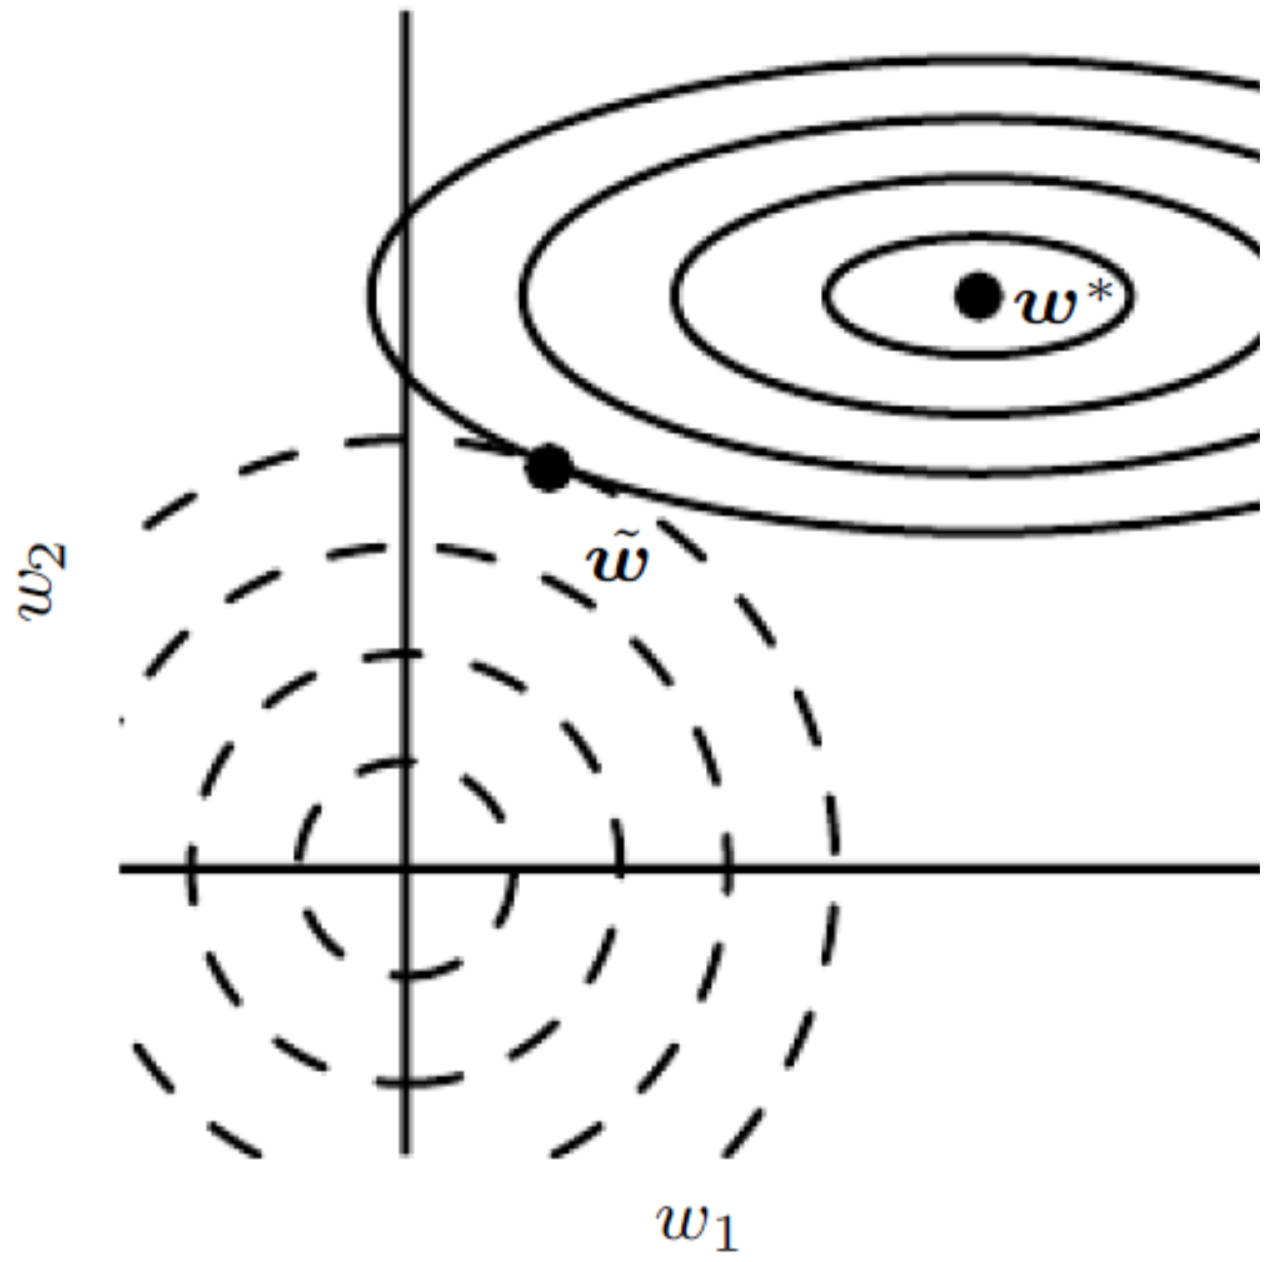
\includegraphics[width=0.5\linewidth]{%
img/l2-regularization-effects-in-risk-space}
\end{center}

The isometric balls illustrate the regularization loss (L2) for any choice of
$\theta$ (or $w$), and the ellipsoid curves illustrate the risk (for
a parabolic risk). So $\tilde{w}$ is the point with the least loss for its
specific regularization loss. As we can see, at that point
\begin{itemize}
  \item downwards the risk has a large eigenvalue, as the risk increases
  rapidly. And as we've stated above, the value of $w$ along that dimension is
  not reduced that much.
  \item from right to left (starting at $w^*$) the risk has a very low
  eigenvalue, and hence $\tilde{w}$ is reduced much more along that dimension.
\end{itemize}

\sep

\Def[L1-Regularization (sparsity inducing)]

$
\Omega(\theta)
=
\sum_{l=1}^L
\lambda^l\norm{\MW^l}_1
=
\sum_{l=1}^L
\lambda^l
\sum_{i,j}
\abs{w_{ij}},
\qquad
\lambda^l\geq 0
$

\sep

\todo{Understand what is mentioned about the one-dimensional problem.}

\todo{Understand connection to batch-normalization with the powers of $\eta$
here\ldots}

\subsubsection{Regularization via Constrained Optimization}

An alternative view on regularization is for a given $r>0$, solve
\[
\min_{\theta, \norm{\theta}\leq r}
\cR(\theta.)
\]
So we're also constraining the size of the coefficients indirecty, be
constraining $\theta$ to some ball.

\ssep

The simple optimization approach to this is: \emph{projected} gradient descent
\[
\theta(t+1)
=
\Pi_r(\theta(t)-\eta\nabla\cR),
\qquad
\Pi_r(\vv):=
\min\set{1,\frac{r}{\norm{\vv}}}\vv
\]
So we're essentially clipping the weights.

\ssep

Actually, for each $\lambda$ in L2-Regularization there is a radius $r$ that
would make the two problems equivalent (if the loss is convex).

\ssep

Hinton made some research in 2013 and realized that
\begin{itemize}
  \item the constraints do not affect the initial learning (as the weights are
  assumed to be small at the beginning), so we won't clip the weights. So the
  constraints only become active, once the weights are large.
  \item alternatively, we may just constrain the norm of the incoming weights
  for each unit (so use row-norms for the weight matrices). This had some
  practical success in stabilizing the optimization.
\end{itemize}

\subsubsection{Early Stopping}

Gradient descent usually evolves solutions from: simple + robust $\to$ complex +
sensitive. Hence, it makes sense to stop training early (as soon as validation
loss flattens/increases). Also: computationally attractive.

Since the weights are initialized to small values (and grow and grow to
fit/overfit) we're kindof clipping/constraining the weight
sizes by stopping the learning process earlier.

Let's analyze the situation closer: If we study the gradient descent
trajectories through a quadratic approximation of the loss around the optimal
set of parameters $\theta^*$. We've derived previously already (and show it
here again with slightly different notation) that:
\[
\evalat{\nabla_{\theta}\cR}{\theta_0}
\approx
\evalat{\nabla_{\theta}\cR}{\theta^*}
+
\evalat{\MJ_{\nabla\cR_{\theta}}}{\theta^*}
(\theta_0-\theta^*)
=
\MH(\theta_0-\theta^*).
\]
This is just because the Jacobian of the gradient map is the Hessian
$\MH_{\cR}$ from before.

So (as seen previously) we have that
\[
\theta(t+1)
=
\theta(t)
-\evalat{\eta
\nabla_{\theta}\cR}{\theta(t)}
\approx
\theta(t)-\eta\MH(\theta(t)-\theta^*).
\]
Now, subtracting $\theta^*$ on both sides gives us
\[
\theta(t+1)-\theta^*\approx
(\MI-\eta\MH)(\theta(t)-\theta^*)
\]
Now we'll use the same trick as before that we can diagonalize the hessian $\MH$
as it's s.p.s.d., so $\MH=\MQ\MLambda\MQ^\T$. Inserting this gives us:
\[
\theta(t+1)-\theta^*\approx
(\MI-\eta\MQ\MLambda\MQ^\T)(\theta(t)-\theta^*)
\]
Now let's have a look at everything w.r.t the eigenbasis of $\MH$, let's define
$\tilde{\theta}=\MQ^\T\theta$. Then
\[
\tilde{\theta}(t+1)-\tilde{\theta}^*\approx
(\MI-\eta\MLambda)(\tilde{\theta}(t)-\tilde{\theta}^*)
\]
Now, assuming $\theta(0)=\vo$ (and inserting and using it) and a small $\eta$
($\forall i\colon \abs{1-\eta\lambda_i}<1$) one gets explicitly
\[
\tilde{\theta}(t)=\tilde{\theta}^* -
\underbrace{(\MI-\eta\MLambda)^t\tilde{\theta}^*}_{\mathclap{\to 0\text{ with
upper ass. on eigenvalues}}}.
\]
Thus (comparing to the previous analysis) if we can choose $t$, $\eta$ s.t.
\[
(\MI-\eta\Lambda)^t\mbeq\lambda(\MLambda+\lambda\MI)^{-1}
\]
\todo{I don't get why we strive for this condition??? It is connected to
something of before\ldots}

\todo{Understand how we get to the next result by doing polynomial
approximations of both sides (see ``Early Stopping: Analysis (Details 1,2 of
2)'')}

which for $\eta\epsilon_i\ll 1$, and $\epsilon_i\ll\lambda$ can be achieved
approximately via performing $t=\frac{1}{\eta\lambda}$ steps.

So early stopping (up to the first order) can thus be seen as an approximate
$L_2$-regularizer.

\subsection{Dataset Augmentation}

Applying some transformations to the input data such that we know that the
output is not affected. E.g., for images: mirroring, slight rotations, scaling,
slight shearing, brightness changes. Blows up data, but: there are approaches to
incorporating this into the gradient instead of the input data.

\subsubsection{Invariant Architectures}

Instead of augmenting the dataset one could build an architecture that is
invariant to certain transformations of the data.

\sep

First, we distinguish the following terms: Let's say we have some $\vx$ and
apply the transformation $\vx':=\tau(\vx)$. Then for our neural network $F$

\begin{itemize}
  \item \Def[Invariance] means that $F(\vx)=F(\tau(\vx))$.
  \item \Def[Equivariance] means that $\tau(F(\vx))=F(\tau(\vx))$.\\
  So applying the transformation before or after applying $F$ doesn't change a
  thing (e.g., convolutions and translations are equivariant).
\end{itemize}

\ssep

E.g. NNs where the first layer is a convolution are invariant to image
translation. Hence, it would make no sense to augment the dataset of images with
translations. It also saves computation and memory not to do this. So if we have
an architecture that is invariant to certain dataset augmentations the
augmentations become obsolete. So, if you can, choose an invariant architecture
to make your life easier in the first place.

\subsubsection{Injection of Noise}

At various places: inputs (noise robustness), weights (regularization), targets
(network becomes more careful)

\subsubsection{Semi-Supervised Training}

If we have a lot of data, but only a few datapoints are labeled. Then
semi-supervised training may become useful. You may build a generative model or
an autoencoder to learn how to represent your data (learn features). Then, we
train a supervised model on top of these representations.

\subsubsection{Multi-Task Learning}

If we have different tasks that we may want to solve, we may share the
intermediate representations across the tasks and then learn jointly (i.e.,
minimize the combined objective). A typical architecture would be to share the
low-level representations, lern the high-level representations per task.

\subsection{Dropout}

\textbf{Dropout idea:} randomly ``drop'' subsets of the units in the network.

So more preciely, we'll define a ``keep'' probability $\pi_i^l$ for unit $i$ in
layer $l$.
\begin{itemize}
  \item typically: $\pi_i^0=0.8$ (inputs), $\pi^{l\geq 1}=0.5$ (hidden units)
  \item realization: sampling bit mask and zeroing out activations
  \item effectively defines an exponential ensemble of networks (each of which
  is a sub-network of the original one), just that we sample these models at
  training-time (instead of during prediction) and we \emph{share} the
  parameters
  \item all modles share the same weights
  \item standard backpropagation applies.
  \item This prevents complex co-adaptions in which a feature detector is only
helpful in the context of several other specific feature detectors. Instead,
each neuron learns to detect a feature that is generally helpful for producing
the correct answer given the combinatorially large variety of internal contexts
in which it must operate. (Hinton et al., 2012). This enforces the features to be redundant (not too specific about one thing in
the image) and also to build on top of \emph{all} the features of the previous
layer (since we never know if some are absent).
\end{itemize}

\textbf{Benefits:} benefits of ensembles with the runtime complexity of the
training of one network. The network gets trained to have many different paths through it to
get the right result (as neurons are turned off).

Equivalent to: adding multiplicative noise to weights or training exponentially
many sub-networks $\sum_{i=1}^{n}\binom{n}{i}=2^n$ wher $n$ is the number of
compute units (so at each iteration we turn some nodes off according to some
probability). So we're getting the benefits of ensembles with the runtime
complexity of just training one network.

Ensembling corresponds to taking geometric mean (instead of usual arithmetic)
(must have to do with exponential growth of networks) of the ensembles:

$
\cProb[\text{ensemble}]{y}{\vx}
=
\sqrt[d]{
\prod_{\mu}
\Prob{\vmu}
\cProb{y}{\vx,\vmu}
}
$

\sep

Having to sample several sub-networks for a prediction is somewhat inconvenient,
so the idea that Hinton et al. came up with is: scaling each weight $w_{ij}^l$
by the probability of the unit $j$ being active 
\[
\tilde{w}_{ij}^l
\gets
\pi_j^{l-1}
w_{ij}
\]
This makes sure that the net (total) input to unit $x_i^{l}$ is calibrated,
i.e.,
\[
\sum_{j}\tilde{w}_{ij}^lx_j^{l-1}
\mbeq
\Exp[Z\sim\Prob{Z}]{
\sum_{j}Z_{j}^{l-1}w_{ij}x_j^{l-1}
}
\sum_{j}\pi_{j}^{l-1}w_{ij}x_j^{l-1}
\qquad\text{\ok}
\]
It can be shown that this approach leads to a (sometimes exact) approximation of
a gemoetrically averaged ensemble (see DL-Book, 7.12).

\sep

\Ex Let's say that at the end we selected each unit with a probability of 0.5.
Then when typically when we're finished with training our neural network, we're
going to multiply all the weights that we obtained with 0.5 to reduce the
contribution of each of the features (since we'll have all of them). So with
this trick for the prediction we can just do a single forward pass.

\sep

\section{Natural Language Processing}

Similarities between text and image processing: local information.

Differences between text and image processing: texts have various lengths, texts
may have long-term interactions, language is a man-made conceptions on how to
communicate with each other / pictures capture the reality, pictures capture the
reality / sentences may mean different things in different contexts

\subsection{Word Embeddings}

\textbf{Basic Idea:} Map symbols over a vocabulary $\cV$ to a vector
representation = \emph{embedding} into an (euclidean) vector space (see lookup
table in architecture overview).

\begin{align*}
\text{embedding map}\colon
\text{(vocabulary) }\cV&\mapsto\R^d\text{ (embeddings)}\\
\text{(symbolic) }w&\mapsto \vx_{w}\text{ (quantitative)}\\
\end{align*}

\[
\text{word }w\in\cV
\to
\text{one-hot }w\in\set{0,1}^{\card{V}}
\to
\text{embedding } \vx_{w}.
\]

$m:=\card{\cV}$, usually $\card{\cV}=10^5$

$d=$ dimensionality of embedding, $d\ll m$ 

So for each of the $m$ words in $\cV$ we have a corresponding embedding in
$\cR^d$, which can be stored in a shared lookup table:

$\cR^{d\times m}$ shared lookup table

Any sentence of $k$ words can then be represented as a $d\times k$ matrix (a
sequence of $k$ embedding vectors in $\R^d$).

\sep

Now, how should an embedding be? Ideally, the embedding carries the
information/structure that we need in order to go from the input text to the
question that we want to solve. Typical questions are:
\begin{itemize}
  \item Clustering based on context (co-occurrence)
  \item Sentiment analysis (group words according to mood/feelings)
  \item Translation (group by meaning)
  \item Part-of-Speech tagging (understand the structure of text, e.g.,
  location, time, actor, \ldots, or, noun, verb, adjective, \ldots) 
\end{itemize}

\ssep

There are three main approaches to construct \emph{sequence embeddings}:
\begin{enumerate}
  \item CNNs
  \begin{itemize}
    \pro conceptually simple, fast to train
    \con limited range of memory 
  \end{itemize}
  \item RNNs
  \begin{itemize}
    \pro active memory management via gated units
    \con more difficult to optimize, larger datasets needed 
  \end{itemize}
  \item Recursive networks (in combination with parsers)
\end{enumerate}



\subsection{Recurrent Networks (RRNs)}

Disadvantage of CNNs: need to pick right convolution size, too small: no
context, too large: a lot of data needed, anyways: loss of memory at some point.

Advantage of RNNs: capture better the time component, lossy memorization of
past in hidden state.

%\begin{center}
%  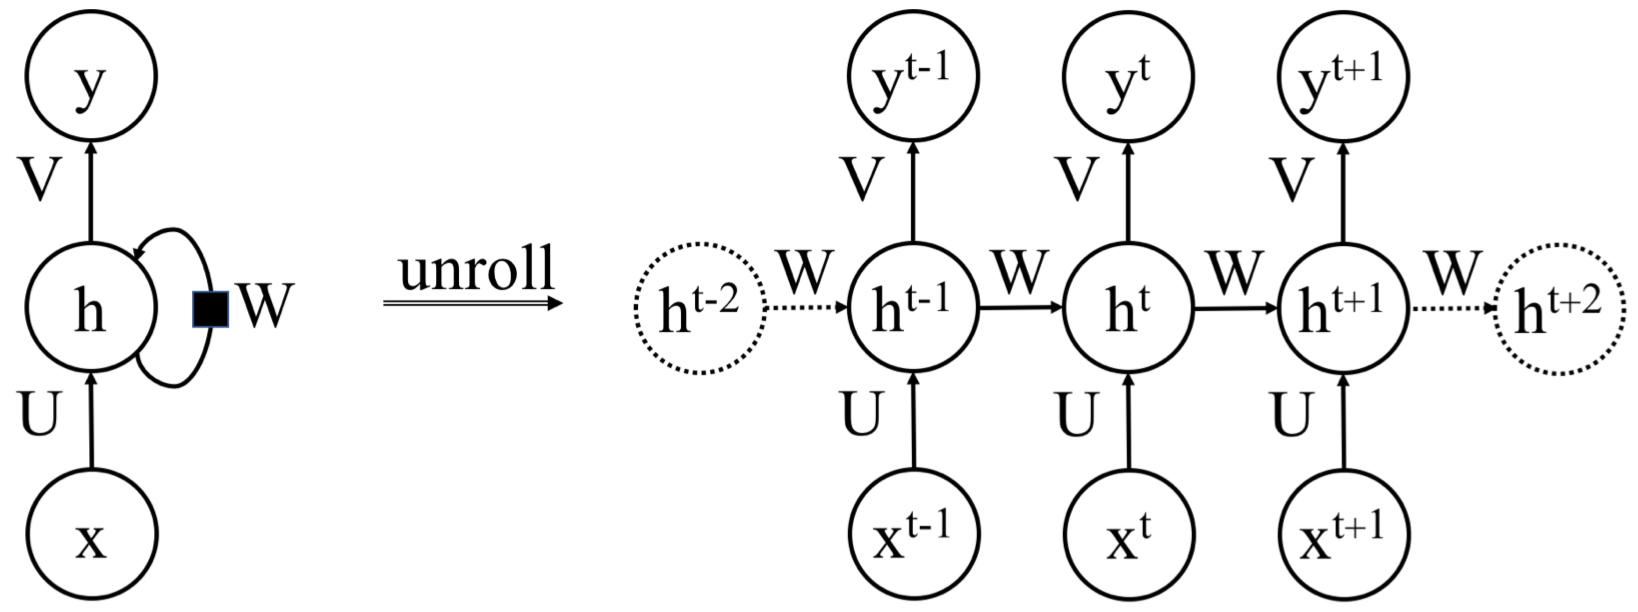
\includegraphics[width=0.6\linewidth]{%
%img/RNN-unfolding}
%\end{center}

Given an observation sequence $\vx^1,\ldots,\vx^T$. We want to identify the
hidden activites $\vh^t$ with the state of a dynamical system. The discrete time
evolution of the \emph{hidden state sequence} is expressed as a HMM with a non-linearity.
\[
\theta=(\MU,\MW,\vb,\MV,\vc)
\]
\[
\vh^t=F(\vh^{t-1},\vx^t;\theta),
\qquad
\vh^0=\vo.
\]
\[
F:=\sigma\circ\overline{F},
\qquad
\sigma\in\set{\text{logistic,tanh,ReLU,\ldots}}
\]
\[
\overline{F}(\vh,\vx;\theta)
:=
\MW\vh+\MU\vx+\vb,
\]
\[
\vy^t=H(\vh^t;\theta):=\sigma(\MV\vh^t+\vc),
\]
There are two scenarios for producing outputs
\begin{enumerate}
  \item Only one output at the end:
  \[
  \vh^T\mapsto\MH(\vh^T;\theta)=\vy^T=\vy
  \]
  And then we just pass this $\vy$ to the loss $\cR$.
  \item Output a prediction at every timestep: $\vy^1,\ldots,\vy^T$. And then
  use an additive loss function
  \[
  \cR(\vy^1,\ldots,\vy^T)=
  \sum_{i=1}^T\cR(\vy^T)=
  \sum_{i=1}^T\cR(H(\vh^T;\theta))
  \]
\end{enumerate}
\begin{itemize}
  \item \textbf{Markov Property:} hidden state at time $t$ depends on input of
  time $t$ as well as the privous hidden state (but we don't need the oder
  hidden states).
  \item \textbf{Time-Invariance:} the state evolution function $F$ is
  independent of $t$ (it's just parametrized by $\theta$).
\end{itemize}

Feedforward VS Recurrent Networks: RNNs process inputs in sequence, parameters
shared between layers (same $H$ and $F$ at every timestep).

\intertitle{Backpropagation in Recurrent Networks}

The backpropagation is straightforward: we propagate the derivatives
\emph{backwards	through time}. So, the parameter sharing leads to a sum over
$t$ when dealing with the derivatives of the weights:

\begin{algorithm}[H]
\caption{Backpropagation in RNNs}
\DontPrintSemicolon
\tcb{(Blue terms only need to be comp. for multiple-output RNNs)}\;
// Compute derivative w.r.t. outputs\;
Compute 
$
\frac{\partial \cR}{\partial \vy^1},
\mcb{\frac{\partial \cR}{\partial \vy^2},
\ldots,
\frac{\partial \cR}{\partial\vy^T}
}$
\qquad
$\left(=\frac{\partial L}{\partial \vy^i}\right)$\; 
// Compute the gradient w.r.t. all hidden states\;
$
\frac{\partial \cR}{\partial \vh^T}
\gets
\sum_{i}
\frac{\partial \cR}{\partial \vy^T_i}
\frac{\partial \vy^T_i}{\partial \vh^T}
$\;
\For{$t\gets (T-1)$ down to $1$}{
$
\frac{\partial \cR}{\partial \vh^t}
\gets
\sum_{i}
\frac{\partial \cR}{\partial \vh^{t+1}_i}
\frac{\partial \vh^{t+1}_i}{\partial \vh^t}
\mcb{+
\sum_{i}
\frac{\partial \cR}{\partial \vy^{t}_i}
\frac{\partial \vy^{t}_i}{\partial \vh^t}}
$\;
}
// Do back-propagation over time for weights and biases\;
$
\frac{\partial \cR}{\partial w_{ij}}
\gets
\sum_{i=1}^T
\frac{\partial \cR}{\partial h_j^{t-1}}
\frac{\partial h_j^{t-1}}{\partial w_{ij}}
=
\sum_{i=1}^T
\frac{\partial \cR}{\partial h_j^{t-1}}
\cdot \dot{\sigma}^t_i
\cdot h_j^{t-1},
$\;
$
\frac{\partial \cR}{\partial u_{ij}}
\gets
\sum_{i=1}^T
\frac{\partial \cR}{\partial h_j^{t-1}}
\frac{\partial h_j^{t-1}}{\partial u_{ij}}
=
\sum_{i=1}^T
\frac{\partial \cR}{\partial h_j^{t-1}}
\cdot \dot{\sigma}^t_i
\cdot x_j^{t},
$\;
$
\frac{\partial \cR}{\partial b_{i}}
\gets
\sum_{t=1}^T
\frac{\partial \cR}{\partial \vh_i^t}
\frac{\partial \vh_i^t}{\partial b_{i}}
=
\sum_{t=1}^T
\frac{\partial \cR}{\partial \vh_i^t}
\cdot \dot{\sigma}^t_i,
$\;
\qquad\qquad\qquad\qquad\qquad\qquad\qquad
where $\dot{\sigma}_i^t:=\sigma'(\overline{F}_i(\vh^{t-1},\vx^t)).$\;
$
\frac{\partial \cR}{\partial v_{ij}}
\gets
\mcb{\sum}_{\mcb{i=1}}^T
\frac{\partial \cR}{\partial y_j^{t-1}}
\frac{\partial y_j^{t-1}}{\partial v_{ij}}
=
\mcb{\sum}_{\mcb{i=1}}^T
\frac{\partial \cR}{\partial y_j^{t-1}}
\cdot \dot{\sigma}^t_i
\cdot y_j^{t},
$\;
$
\frac{\partial \cR}{\partial c_{ij}}
\gets
\mcb{\sum}_{\mcb{i=1}}^T
\frac{\partial \cR}{\partial y_j^{t-1}}
\frac{\partial y_j^{t-1}}{\partial v_{ij}}
=
\mcb{\sum}_{\mcb{i=1}}^T
\frac{\partial \cR}{\partial y_j^{t-1}}
\cdot \dot{\sigma}^t_i,
$\;
\qquad\qquad\qquad\qquad\qquad\qquad\qquad
where $\dot{\sigma}_i^t:=\sigma'(\overline{H}_i(\vh^{t-1},\vx^t)).$\;
\end{algorithm}

\todo{Think about how to write these in matrx form}

Note that
$
\frac{\partial \cR}{\partial w_{ij}}
\gets
\sum_{i=1}^T\sum_{k}
\frac{\partial \cR}{\partial h_k^{t-1}}
\frac{\partial h_k^{t-1}}{\partial ww_{ij}}
=
\sum_{i=1}^T
\frac{\partial \cR}{\partial h_j^{t-1}}
\frac{\partial h_j^{t-1}}{\partial w_{ij}}
$.
Since for $k\neq j$ the summand is zero (similarly for $u_{ij}$ and $v_{ij}$).

\intertitle{Exploding and/or Vanishing Gradients}

One of the typical problems that RNNs have is that the gradients may explode or
vanish. Remember that the gradients that we with MLPs were:
\[
\nabla_{\vx}\cR=\MJ_{F^1}\cdot\cdots\cdot\MJ_{F^L}\nabla_{\vy}\cR.
\]
Since we're sharing the parameters we have $\forall t\colon F^t=F$, yet
evaluated at different points. Now, if the sequence is very long (large $T$)
then we're multiplying a lot of times the same jacobian (yet evaluated at
different points) by itself.



\subsubsection{Backprop Over Time}

For multi-output loss

$
\frac{L}{\theta}
=\sum_{t=1}^T
\frac{\partial L_t}{\partial y_t}
\frac{\partial y_t}{\partial h_t}
\sum_{\ell=1}^T
\left[
\prod_{k=\ell+1}^T
\frac{\partial h_k}{\partial h_{k-1}}
\right]
\frac{\partial h_t}{\partial \theta}
$


\subsubsection{Bi-Directional RNNs}

\begin{center}
  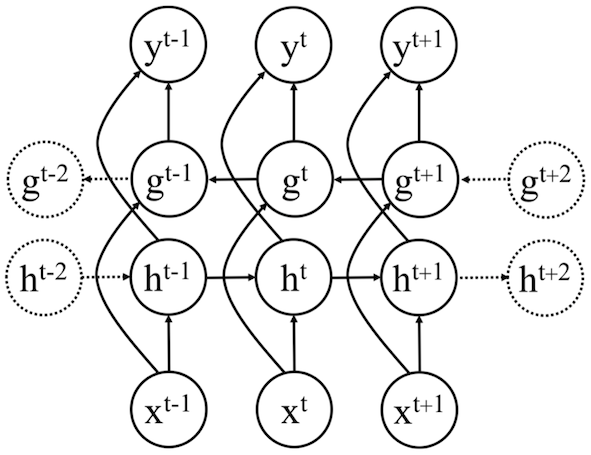
\includegraphics[width=0.2\linewidth]{%
img/bi-directional-rnn}
\end{center}

So, additionally, we're define a \emph{reverse order sequence}
\[
\vg^t:=G(\vx^t,\vg^{t+1};\theta)=\sigma(\MP\vx^t+\MQ\vg^{t+1}+\vd),
\quad\text{with }\vg^T=\vo
\]
the function $F$ to compute the normal order sequence stays the same, and the
output transform $H$ becomes now a function of both hidden states:
\[
\vy^t=H(\vh^t,\vg^t;\theta).
\]
The nice thing is that we can compute both sequences (the forward and backward
sequence) in parallel (or independently) - just verify this in the graph. The
back-propagation through time is done in reverse order for the reverse order
sequence.

\subsubsection{Deep Recurrent Networks}

Deep recurrent networks (DRNNs) just use a deeper network for the evolution
function. So we have hierarchical hidden states. Note, that this can also be
combined with bi-directionality.

\begin{multicols}{2}
\begin{align*}
\vh^{t,1}&=F^(\vh^{t-1,1},\vx^t;\theta)\\
&\,\,\,\,\vdots\\
\vh^{t,l}&=F^(\vh^{t-1,l},\vh^{t,l-1};\theta)\\
\vy^T&=H(\vy^{t,L};\theta).
\end{align*}
\begin{center}
  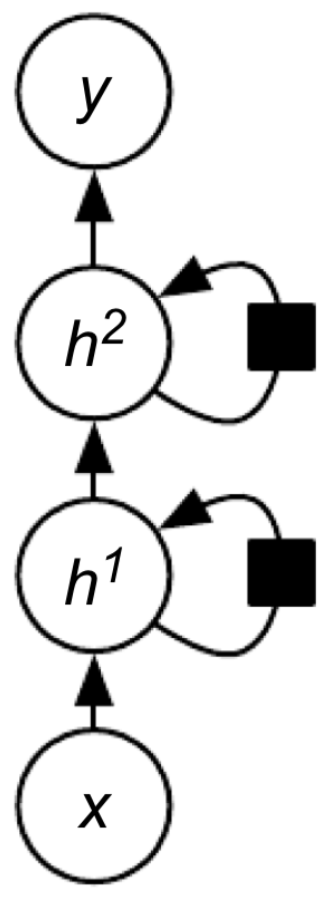
\includegraphics[width=0.2\linewidth]{%
img/DRNN}
\end{center}
\end{multicols}





\subsubsection{Probability Distributions over Sequences}

\textbf{Goal}: Define a conditional probability distribution over output
sequence $\vy^{1:T}$, given input sequence $\vx^{1:T}$.

So the idea would be to do a step-by-step prediction:
\[
\cProb{\vy^{1:T}}{\vx^{1:T}}
\approx
\prod_{t=1}^T
\cProb{\vy^t}{\vx^{1:t},\vy^{1:(t-1)}}
\]
Now, in the naive RNN implementation $\Prob{\vy^t}$ only depends on
$\vy^{1:(t-1)}$ through $\vh^t$ since
\[
\vx^{1:t}
\stackrel{F}{\mapsto}
\vh^T
\stackrel{H}{\mapsto}
\vmu^t
\mapsto
\Prob{\vy^T}.
\]

\textbf{Problems when learning RNNs} One of the problems that we may have when
we're learning to predict sequences to sequences is that the elements of the
predicted sequence are somewhat un-correlated if we don't train the right way.
Actually, it would be better to consider what we predicted for the neighbouring
elements when predicting an element of a sequence. Further, if the prediction
was wrong it would be actually misleading, and so the error would get
propagated. A better approach to do this is to feed in the right prediction as
the neighbouring prediction during training time such that the training and
sequence doesn't get fully of track because of one misprediction.

\sep



\Def[Curriculum Learning] Another related idea is \emph{curricular learning}
where we alternate randomly between teacher forcing and using the actual (and
maybe wrong) prediction. So even if there are some wrong predictions, we force
the network to come to the right prediction at some point and it may recover
from the small errors.


\section{Memory \& Attention}

\subsection{Memory Units}

\textbf{Problem with RNNs:} vanishing gradients (changes in the input a long
time ago won't really affect the output/loss), so it's hard to learn long-term
dependencies as the information in $\vh_t$ fades-out when combined with current
input $\vx_t$.

\textbf{Goal of Memory Units:} model long-term dependencies. have some kind of
memory.

\subsubsection{LSTMs}

It would be nice to have something like a gated unit

\sep

\Def[Gated Unit]

The following picture illustrates how we have a memory unit where we can store,
read and delete information illustrated by the \emph{gated units}.

\begin{center}
  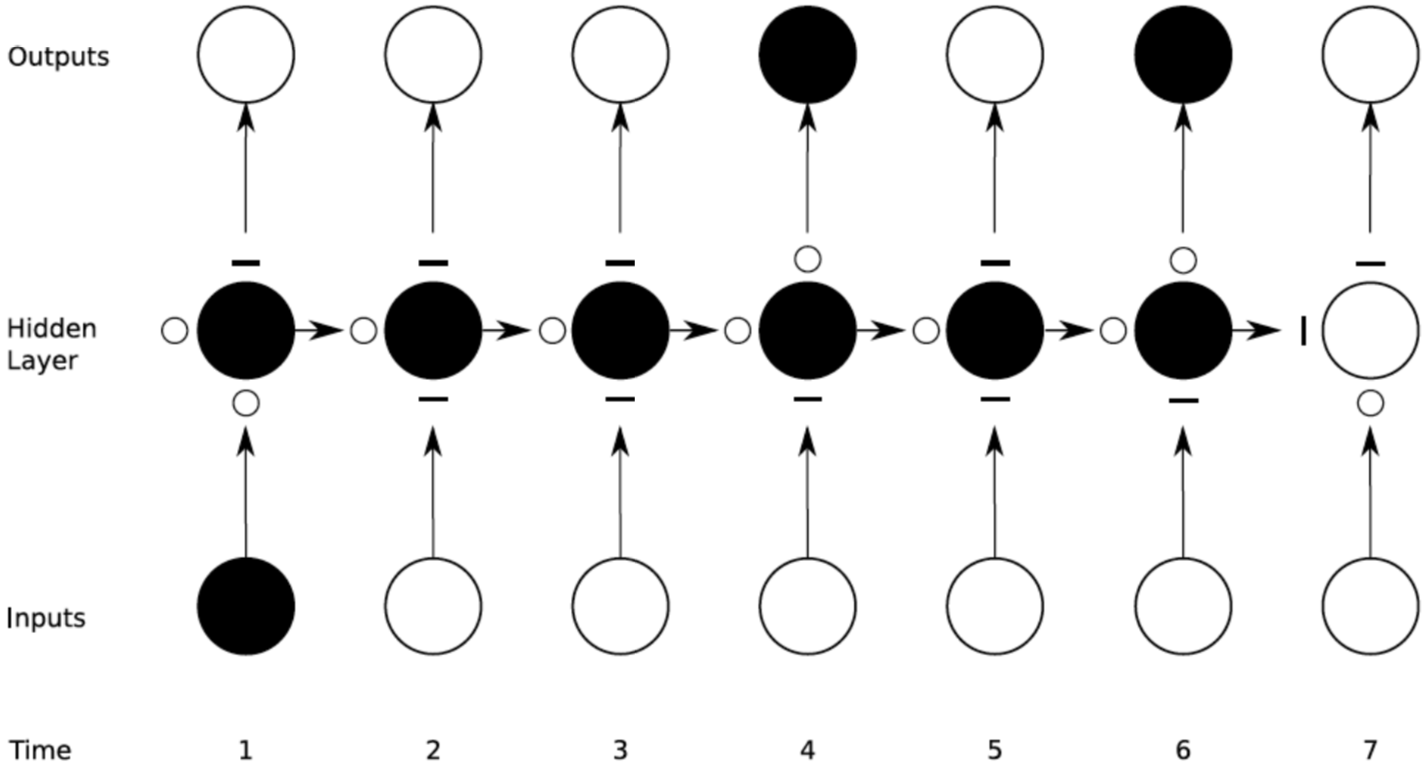
\includegraphics[width=0.6\linewidth]{%
img/memory-units}
\end{center}

Advantages: information can be remembered for a long time (doesn't fade away as
with RNNs). Further, we can delete something in memory in one timestep
(without having to fade it out). 

\sep

\Def[LSTM] Long Short-Term Memory: Remembering information for long time and
forgetting it fast.

An LSTM is just a complex unit for memory management to achieve these
objectives. It has the following computation graph:

\begin{center}
  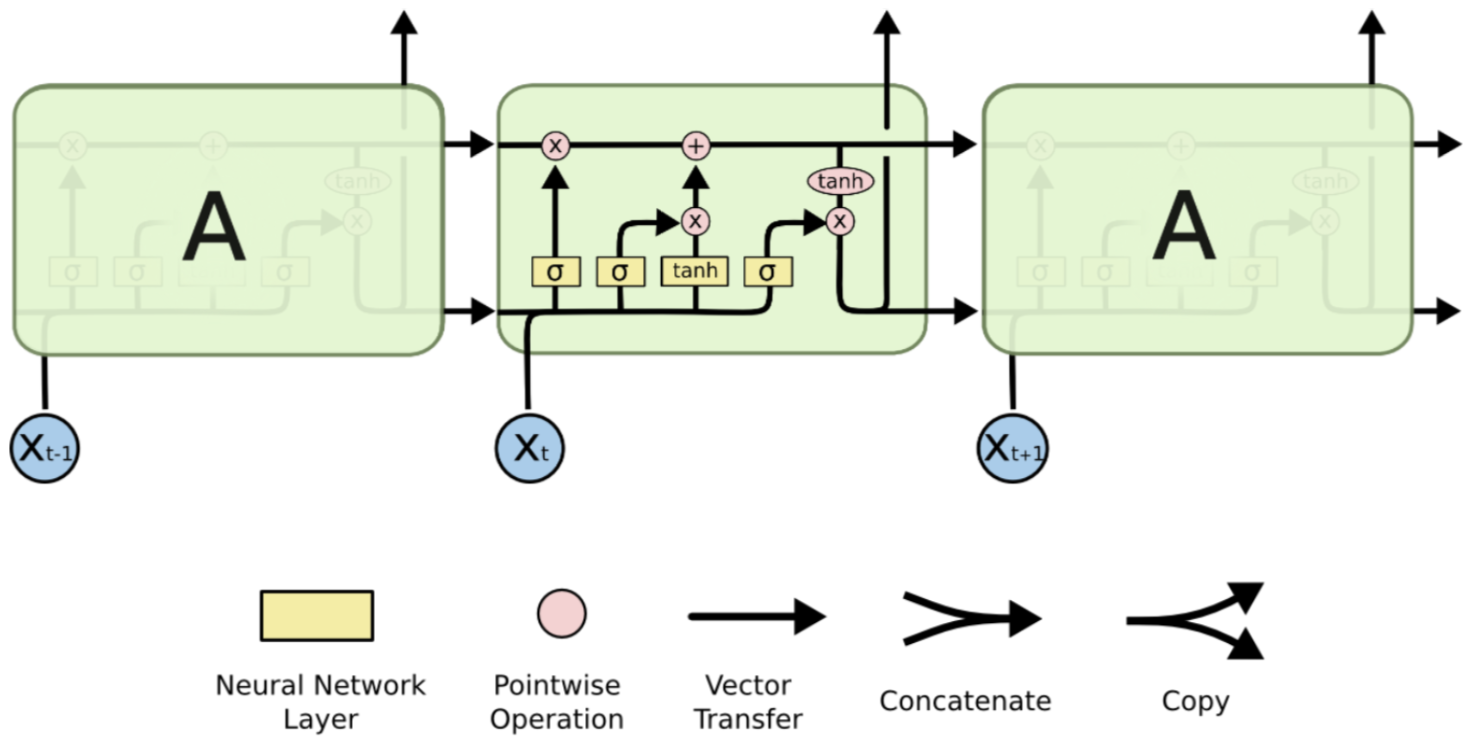
\includegraphics[width=1\linewidth]{%
img/lstm}
\end{center}

Now an LSTM has two memories:
\begin{itemize}
  \item $C_t$ is the \emph{main memory} in the LSTM (a vector). That's where we
  store all of our information. The memory we'll control through the gated
  units.
  \item $h_t$ is our previous output. So it's not our memory, but it's what the
  sequence model outputs at timestep $t$. This could then passed further to a
  prediction network.
\end{itemize}

\begin{center}
  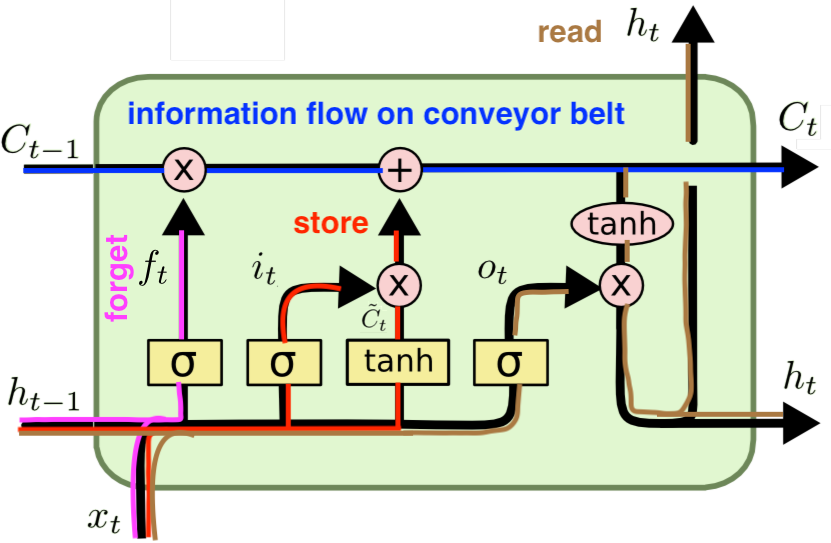
\includegraphics[width=1\linewidth]{%
img/lstm-combined-v3}
\end{center}

The LSTM adds three more gates. The idea is that the information $C_t$ flows on
a \textbf{\tcb{conveyor-belt}} where we selectively forget, store and output as
follows

\begin{itemize}
  \item \textbf{\textcolor{RubineRed}{Forget Gate:}} This is just a one-layer
  neural network, where
  \[
  \vf^t=\sigma(\MW_f\vh^{t-1}+\MU_f\vx^t+\vb_f)
  \qquad(\vf\text{orget})
  \]
  Using the previous output vector, and the current input it computes some
  weights, which are used to multiply the content of the memory (by a number
  between 0 and 1) in order to selectively forget some entries in the memory.
  \item \textbf{\tcr{Store/Input Gate:}} Here we'll compute
  \[
  \vi^t:=\sigma(\MW_i\vh^{t-1}+\MU_i\vx^t+\vb_i)
  \qquad(\vi\text{nput})
  \]
  which determines how much we want to input into the memory (how much we want
  to store). 
  In many cases, this is just mapped as $\vi^t=1-\vf^t$. But this
  model illustrates the flexibility that we may want to keep. Further, given
  that we'll be opening the gate, what should we store there? This is what is
  computed through
  \[
  \overline{C}^t=\tanh(\MW_C\vh^{t-1}+\MU_C\vx^t+\vb_C).
  \]
  And in the end we'll update the memory by combining the weighted sums of
  the stored and new information
  \[
  C^t=\underbrace{\vf^t}_{\text{forget factors}} \odot
  \underbrace{C^{t-1}}_{\text{current mem}} + \underbrace{\vi^t}_{\text{write
  factors}} \odot\underbrace{\overline{C}^t}_{\text{net in}}.
  \]
  \item \textbf{\textcolor{brown}{Read/Output Gate:}} In this gate we decide
  which information that we want to get out into our output (the new hidden
  state):
  \[
  \vo^t=\sigma(\MW_o\vh^{t-1}+\MU_o\vx^t+\vb_o)
  \qquad(\vo\text{utput})
  \]
  \[
  \vh^t=\underbrace{\vo^t}_{\substack{\text{what we want}\\\text{to let
out}}}\odot\tanh(\underbrace{C^t}_{\text{new mem.}}).
  \]
\end{itemize}

\sep

Note that when stacking $\vh^{t-1}$ and $\vx^t$ we may just represent things as
follows:

\[
\begin{bmatrix}
\MW^\kappa & \MU^\kappa
\end{bmatrix}
\begin{bmatrix}
\vh^{t-1}\\
\vx^{t}
\end{bmatrix}
+\vb^\kappa
=
\MW^k\vh^{t-1}+\MU^k\vx^t
+\vb^\kappa.
\]

\intertitle{GRU Networks (Gated Memory Unit)}

\begin{center}
  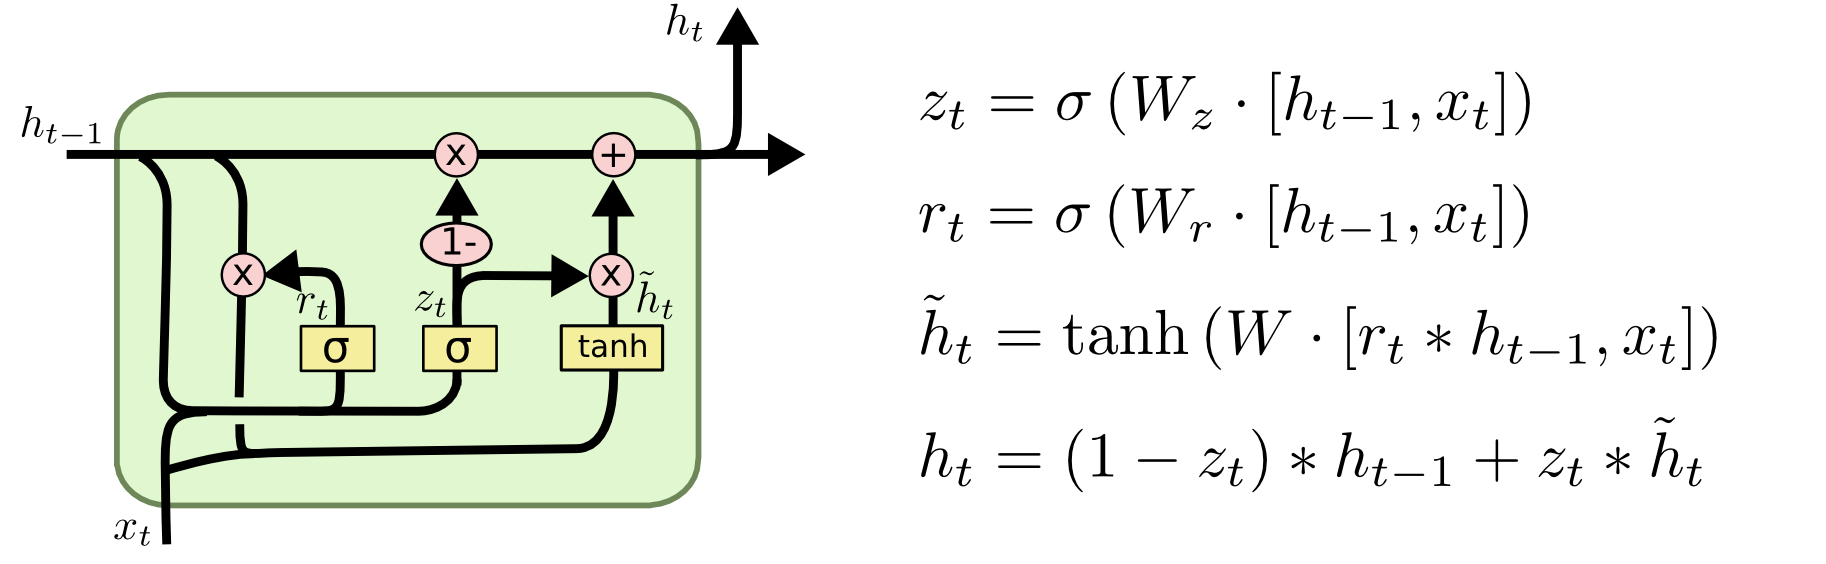
\includegraphics[width=1\linewidth]{img/lstm-grus}
\end{center}

This is basically a simplification of the LSTM that we've seen where we have
only one state. Usually these ones tend to be much faster to train. It combines
the forget and input gates into a single ``update gate.'' It also merges the
cell state and hidden state, and makes some other changes.


\subsection{Differentiable Memory}

\Def[Neural Turing Machine]

NTMs are very reminiscent of a Turing machine, but: each cell $M_i\in\R^d$.

\begin{center}
  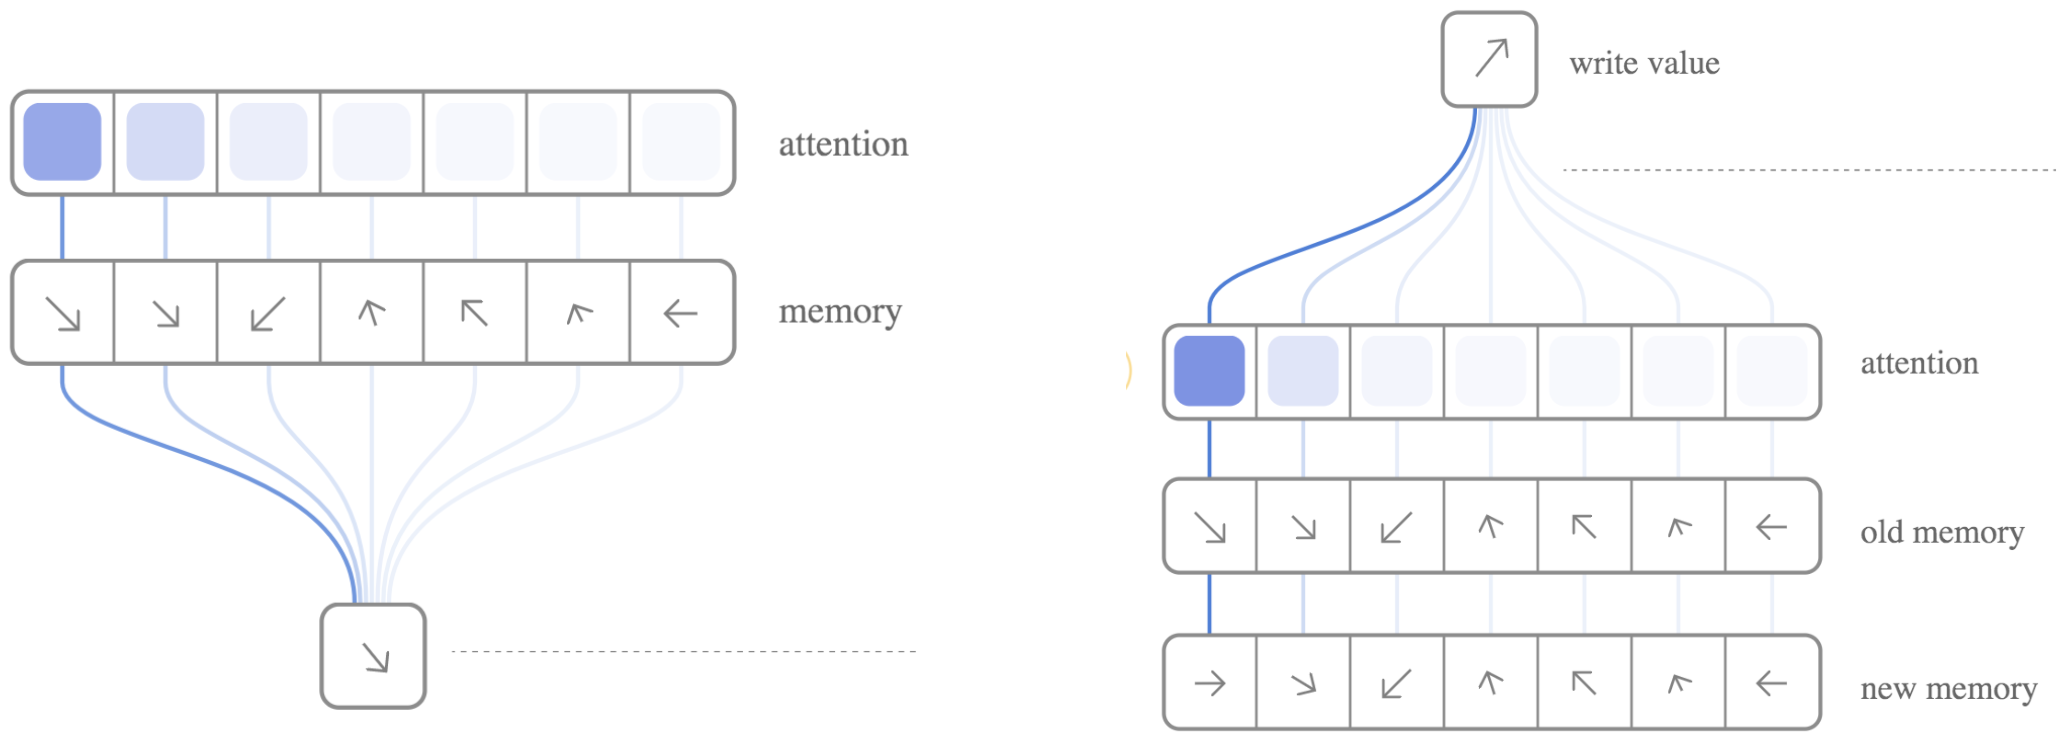
\includegraphics[width=0.7\linewidth]{%
img/ntms-1}
\end{center}

In contrast to RNNs, NTMs use an external memory to which they read and write
according to some determined probabilities.Now here's an example how that can become very useful. We may have these vectors
in memory, and then we may search for some vector. The greater the dot-product
is with a vector, the greater our attention will be for that vector in the
memory (via the attention distribution). 

So the operations that can be done are the following:
\begin{enumerate}
  \item Compute the attention distribution: $(\alpha_i)_i$, $\alpha_i\geq 0$
  s.t. $\sum_{\alpha_i}=1$.
  \item Read: out expected memory content: $r\gets\sum_i \alpha_iM_i$.
  \item Write: Now, given that we have one value that we'd like to write, we'll
  write it to the memory location with the biggest attention:
  \[
  (\beta_i)_i,\quad \beta_i\in[0;1],\quad M_i\gets(1-\beta_i)M_i+\beta_iw.
  \]
  Usually, there's one value where we have a lot of attention (curse of
  dimensionality), and lots where we have little attention. Further, as we can
  see then we'll write a lot so somwhere and a little bit to everywhere else.
  The reason we're using a slowly varying $\beta_i$ is that we want to be able
  to take the derivative (if it was just 0 or 1 we couldn't take the
  derivative). So this is why these things tend to be soft.
\end{enumerate}

The typical memory controller works as follows:
\begin{center}
  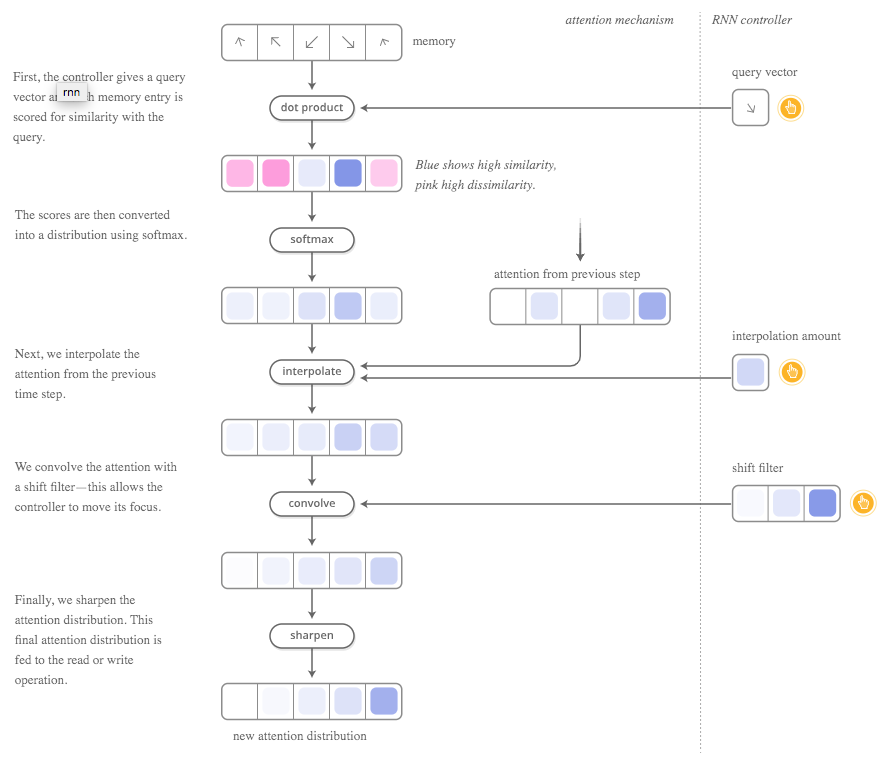
\includegraphics[width=0.5\linewidth]{%
img/ntms-2}
\end{center}

\begin{enumerate}
  \item For a \emph{query} vector see which memory cells get the most attention.
  \item Normalize the attention distribution
  \item Interpolate the attention with the previous attention
  \item Convolve the the attention if needed (ability to shift attention
  relative to content-selected locations)
  \item additionally sharpen the final attention distribution.
  \item then do your operation (read or write) according to the attention
  distribution.
\end{enumerate}

These operations are all differentiable, as we're using probabilities and not
only the values 0 or 1. Other resembling architectures are: neural random access
machines, differentiable data structures (stacks, queues).

Now, NTM architectures can learn loops and simple programs. However, no
real-world applications have been developed with this so-far.

\subsection{Attention Mechanisms}

\Def[Attention Mechanisms] offer a simple way to overcome some challenges of
RNN-based memorization. With attention mechanisms we selectively attend to
\emph{inputs} or \emph{feature representations} computed from inputs.

\begin{itemize}
  \item RNNs: learn to encode information relevant for the future.
  \item Attention: selects what is relevant from the past in hindsight!
\end{itemize}
Both ideas can be combined!

\sep

\Ex If we have a sentence in English and one in German the question is how do we
match one to the other. The problem with CTC was that if things are changed in
order, then CTC cannot deal with it. Because the CTC doesn't process every input
before it produces an output. Attention will provide a mechanism to deal with
this.

\sep

So we'll see how we can do sequence to sequence learning. The idea fairly
simple: Let's say we have a sequence $ABC$ and we want to map it to $WXYZ$. To
acheve this we'll use the so-called \emph{encoder-decoder architecture}:

\begin{center}
  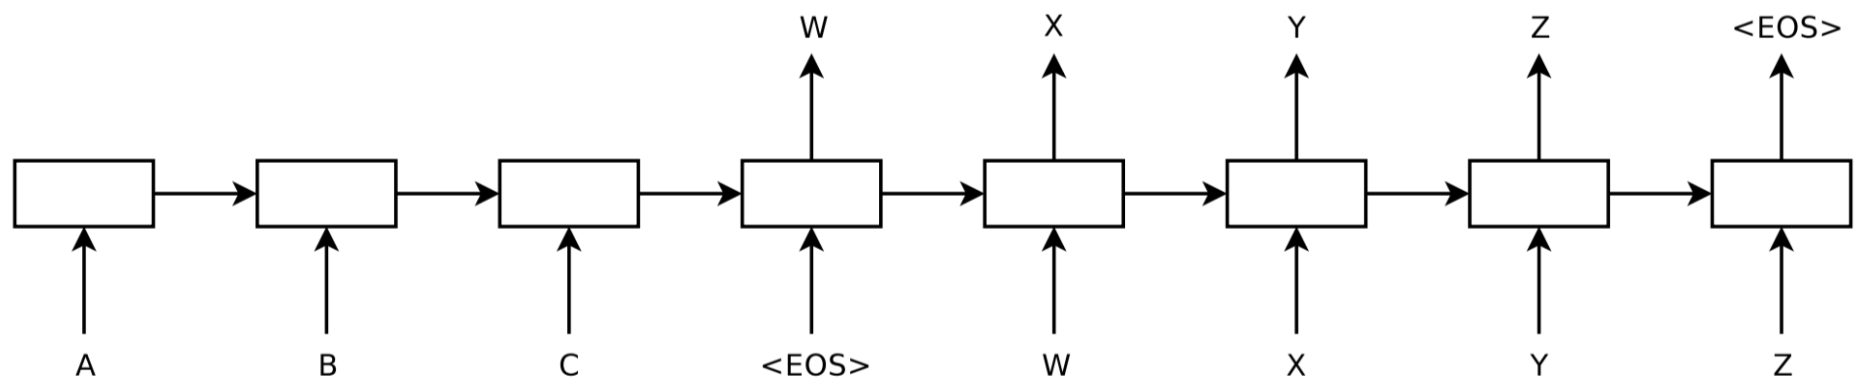
\includegraphics[width=1\linewidth]{%
img/seq-to-seq-encoder-decoder}
\end{center}

So what we'll do is
\begin{itemize}
  \item we'll \emph{encode} the sequence (e.g., sentence) into a vector, and
  then
  \item we'll \emph{decode} the sequence (e.g., translate) from the vector (w/
  output feedback) into another sequence.
\end{itemize}

So the probability that we want to determine is
\[
\cProb{\vy^1,\ldots,\vy^{T_y}}{\vx_1,\ldots,\vx^{T_x},F(\vx^{T_x})}.
\]
The issue that we have here is that $T_x$ and $T_y$ have variable lengths, and
the difference between the two lengths is not always the same. So it's very hard
to match one sequence to another. Now, sequence learning will compute a function
\[
F(\vx^1,\ldots,\vx^{T_x}) = \text{``thought vector''}
\]
which will be a vector which will have all the information that we need from the
input sequence to compute the output sequence. This $F$ is the so-called
``thought vector'' (Hinton). So $F$ will be computed via an LSTM. 

To produce the output sequence we'll use another LSTM that takes as input the
thought vector $F$ plus the output that we'll be producing (output feedback).

\intertitle{How to make the RNN Encoder/Decoder Work?}

The following things were discovered by Sutskever, Vinals \& Le in 2014:
\begin{itemize}
  \item Use Deep LSTMs (multiple layers, e.g., 4)
  \item Use different RNNs for encoding and decoding
  \item Apply beam search for decoding
  \item Reverse the order of the source sequence
  \item Ensemble-ing
\end{itemize} 

For a machine translation task this gave state-of-the-art results on WMT
benchmarks. However, traditional approaches use \emph{sentence alignment
models}. We still don't know what is the equivalent in a neural architecture.

\subsubsection{Seq2Seq with Attention}

The issue with the encoder-decoder architecture is that if we're translating a
very long sequence, it might have the issue that suddenly we have to store the
entire sequence in a single vector. But when we as humans translate we translate
small parts into small parts. In order to understand this better let's have a
look at a concrete example. Let's say that we want to translate the following
sentence from English to French.
\begin{itemize}
  \item bi-directionality (it's good to know future and past context)
  \item select useful hidden states based on atention
  \item sizes of sentences might not be the same
  \item outputted workds might have slightly different order
  \item Note that if we don't have dependencies that are out of order we can use
  the CTC approach.
\end{itemize}

\begin{comment}
\subsection{Memory Networks}

Let's consider the following examples.

\begin{center}
  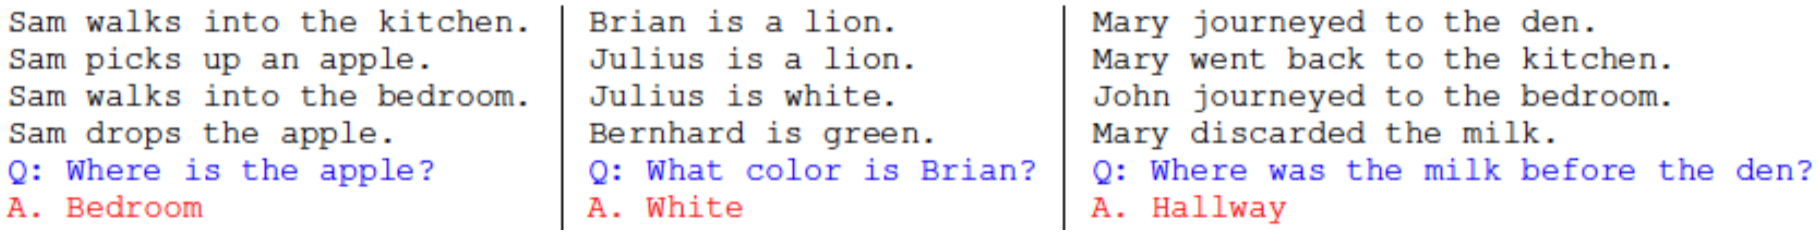
\includegraphics[width=1\linewidth]{img/memory-networks-use-case}
\end{center}

In each of these examples we have a piece of information and then we get a query
that we have to answer. So we have to read a text, and then we'll get a question
about it. This is what memory networks try to achieve.

So, the approach that was taken (by Weston et al, 2014; Kumar et al, 2015) is
the following:
\begin{itemize}
  \item operate over a large data corpus (e.g., text documents)
  \item given a question, learn to infer the answers (QA retrieval)
  \item simplest form: memory is not altered
  \item \emph{recursive associative reall:} given a query $q$, find the best
  matching memory cee $i$; use $M_i$ and $\vx$ as a new key; repeat
\end{itemize}



\begin{center}
  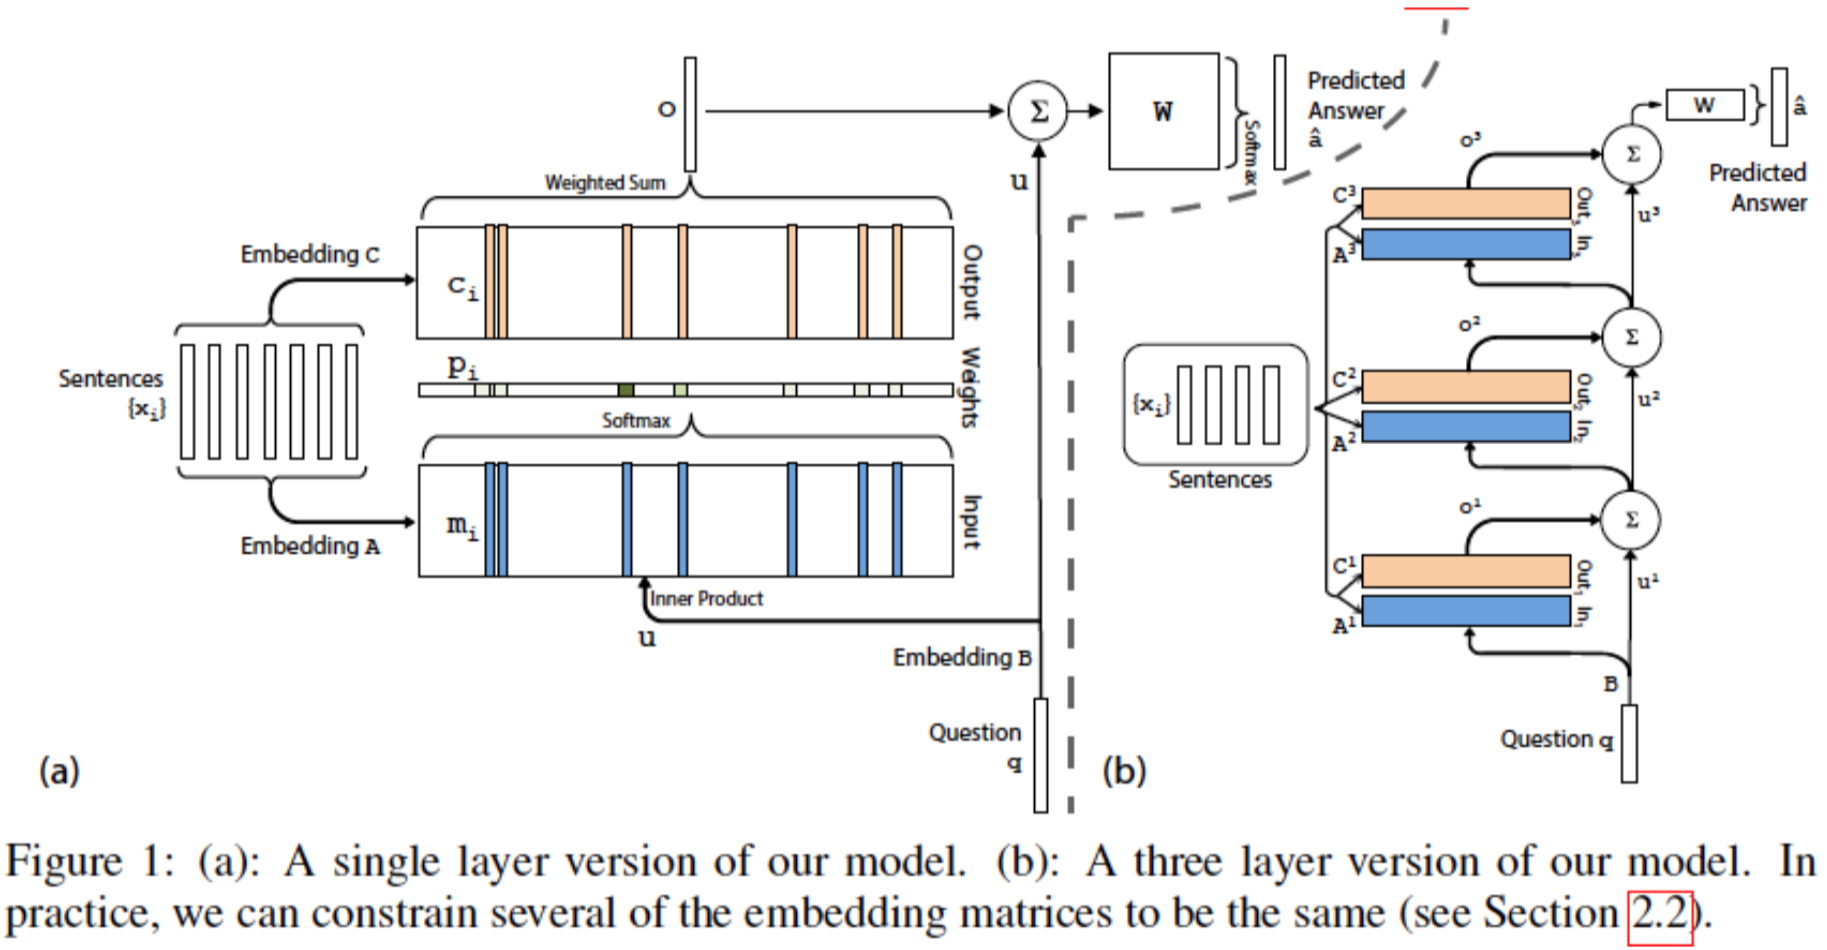
\includegraphics[width=1\linewidth]{img/memory-network-architecture}
\end{center}

So we'll first embed every word by word into a memeory. And then, \todo{what??}.

Then we'll get a question $q$ which we'll use to recover the relevant
information from the memory. This will give us some softmax output that will
tell us which of the pieces that are relevant.

\todo{I didn't understand the part with the output.}

So what we'll be training ar the three embeddings (A, B, C). 

So that's an architecture that we may use when building a chatbot.

\todo{Find out equations that were given.}

\sep

Note how again here the architecture encodes a lot of prior knowledge about the
problem. Once we've found this architecture we can just do end-to-end learning
and do not have to worry about anything. The next steps in deep learning will be
to figure out whether we can build NNs that figure out these architectures by
themselves.
\end{comment}

\subsection{Recursive Networks}

Good to process tree-structure, e.g., from a parser (more depth efficient
$\BigO(\log(n))$). Gives a single output at the root.

$F\colon\R^d\times\R^d\to\R^d$

$\vh^n=F(\vh^{n_{\text{left}}},\vh^{n_{\text{right}}})$

\section{Unsupervised Learning}

Here we'll look at what we can say about a distribution of $\rvX$, when we have
some samples $\vx_1,\ldots,\vx_N$. Unsupervised learning is the most dangerous
thing that we can do (dangerous if we don't know what we're doing). Unsupervised
learning usually is hard, because we don't have a goal. The final goal of
unsupervised learning is \emph{density estimation} - so, understand the
distribution that the data is coming from. Other things we might strive for is
interpretability of the results we've learned about $p(x)$. Another key aspect
of unsupervised learning is: ``I don't know what I'm looking for until I find
it.''

\sep

\todo{Have a look at the example algorithm: ``Latent Dirichlet Allocation'' A
clustering algorithm for documents. This is a very useful algorithm if we're
trying to summarize documents and trying to understand what there is in these
documents. We'll come to LDA back later.}

\subsection{Autoencoders}

\textbf{Given:} data points $\set{\vx_1,\ldots,\vx_n}\subset\R^d$

\textbf{Goal:} \emph{Compress} the data into $m$-dim. $(m\leq d)$
representation.

\sep

\Def[Autoencoder] any NN that aims to learn the \emph{identity map}.
\[
\cR(\theta)=\frac{1}{2n}\sum_{i=1}^n\norm{\vx-F_\theta(\vx)}_2^2
=\Exp[\vx\sim p_{\text{emp}}]{\ell(\vx,(H\circ G)(\vx))}
\]
\[
\ell(\vx,\hat{\vx})=\frac{1}{2}\norm{\vx-\hat{\vx}}^2_2
\]
Typically, the network can be broken into two parts $G$ and $H$ such that
\begin{itemize}
  \item $F=H\circ G\approx \vx\mapsto\vx$
  \item \emph{Encoder}: $G=F_l\circ\cdots\circ F_1\colon\R^n\to\R^m$,
  $\vx\mapsto\vz=\vx^l$
  \item \emph{Decoder}: $H=F_L\circ\cdots\cric F_{l+1}\colon\R^m\to\R^n$,
  $\vz\mapsto\vy=\hat{\vx}$.
  \item layer $l$ is usually a ``bottleneck'' layer.
\end{itemize}

\Com Just a special case of a feedforward NN, that can be trained through
backpropagation.

\sep

Autoencoders provide a canonical way of \emph{representation learning} (since
NNs naturally do this). Note, how the data compression (learning compressed
representation) is just a ``proxy'' and not the real learning objective of the
network (identity function).

\subsubsection{Linear Autoencoding}

\Def[Linear Autoencoder]

A linear autoencoder just consists of two linear maps: an encoder
$\MC\in\R^{m\times d}$ and a decoder $\MD^{d\times m}$. The objective it
minimizes is then:
\[
\cR(\theta)
=
\frac{1}{2n}
\sum_{i=1}^n
\norm{\vx_i-\MD\MC\vx_i}_2^2.
\]

So it's a NN with one hidden layer (no biases and linear activation
functions) which will contain the compressed representation
$\vz=\MC\vx\in\R^{m}$.

\sep

\Def[Linear Autoencoder with Coupled Weights] 

Then, we define $\MD:=\MC^\T$.

\sep

\Def[Singular Value Decomposition]

\todo{Define this cleanly!!!!}

\todo{Define this cleanly!!!!}

\todo{Define this cleanly!!!!}

Recall that the SVD of a data matrix
\[
\MX=
\begin{bmatrix}
\vertbar & \vertbar & & \vertbar\\
\vx_1 & \vx_2 & \cdots & \vx_k\\
\vertbar & \vertbar & & \vertbar\\
\end{bmatrix}
\]
is of the following form:
\[
\MX
=
\underset{n\times n}{\MU}
\underbrace{
\diag^\dagger(\sigma_1,\ldots,\sigma_{\min(n,k)})
}_{=:\MSigma\in\R^{n\times k}}
\underset{k\times k}{\MV^\T}.
\]
And the matrices $\MU$ and $\MV$ are orthogonal - so we have an orthogonal
basis. Further recall that via the SVD we can get the best rank $k$
approximation of a linear mapping. It also is a decomposition that preserves as
much of the variance (or energy) of the data for a predefined number of desired
basis vectors to represent it.

\intertitle{Optimal Linear Compression}

\Thm[Eckhart-Young] For $m\leq\min(n,k)$ and the objective
\[
\argmin_{\hat{\MX}\colon\rank(\hat{\MX})=m}
\norm{\MX-\hat{\MX}}_F^2
=\MU_m
\diag(\sigma_1,\ldots,\sigma_m)
\MV_m^\T
\]
where the subscript $m$ refers to the matrices of the SVD pruned to $m$ columns.

\ssep

\Cor This means that a linear auto-encoder with $m$ hidden units cannot improve
the SVD since $\rank(\MC\MD)\leq m$. However, the auto-encoder can achieve the result of
the SVD.

\ssep

\Thm Given the SVD of the data $\MX=\MU\diag(\sigma_1,\ldots,\sigma_n)\MV^\T$.
The choice $\MC=\MU^\T_m$ and $\MD=\MU_m$ minimizes the squared reconstruction
error of a two-layer linear auto-encoder with $m$ hidden units.

\Proof
\begin{align*}
\MD\MC\MX
=
\MU_m\MU_m^\T\MU\MSigma\MV^T
=
\MU_m\begin{bmatrix}\MI_m & \MO\end{bmatrix}\MSigma\MV^T
=
\MU_m\begin{bmatrix}\MSigma_m & \MO\end{bmatrix}\MV^T
=
\MU_m\MSigma_m\MV_m^T.
\end{align*}
And as we know from the Eckhart-Young theorem $\hat{\MX}=\MU_m\MSigma_m\MV_m^T$
is the best $m$-dimensional approximation of the original data $\MX$. 

Now, since $\MC=\MU_m^\T$ and $\MD=\MU_m$ that means that we can do weight
sharing between the decoder and encoder network, since $\MC=\MD^\T$.

Another thing to note is that the solution is \emph{not unique!} For any
invertible matrix $\MA\in GL(m)$ we have
\[
\underbrace{(\MU_m\MA^{-1})}_{\tilde{\MD}}
\underbrace{(\MA\MU_m^\T)}_{\tilde{\MC}}=\MU_m\MU_m^\T
\]
Now, restricting through weight sharing that $\MD=\MC^\T$ will enforce that
\[
\MA^{-1}=\MA^\T
\]
hencem $\MA\in O(m)$ (orthogonal group, rotation matrices). Then the mapping
$\vx\to\vz$ is determined (up some rotation that we do in-between, rotation and
its inverse).

\intertitle{Principal Component Analysis}

\todo{Define this cleanly!!!!}

\todo{Define this cleanly!!!!}

\todo{Define this cleanly!!!!}

A way to solve \todo{thsi problem, which?? the rotation??} this problem is
through PCA. First, we center the data (pre-processing) as follows:
\[
\vx_i
\mapsto
\vx_i
\sum_{i=1}^k
\vx_i
\]
Then we define
\[
\MS:=\MX\MX^\T
\]
which is the sample covariance matrix. And then, in order to get $\MU$ we just
do the singular value decomposition of $\MS$. If we relate it to the SVD of
$\MX$ we can see that
\[
\MS=\MU\MSigma\MV^\T\MV\MSigma\MU^\T=\MU\MSigma^2\MU^\T.
\]
So, the column vectors of $\MU$ are the eigenvectors of the covariance matrix.
And $\MU_m\MU_m^\T$ is the orthogonal projection onto $m$ principal components
of $\MS$.

\todo{Might there also be efficiency reasons for doing the PCA instead of the
SVD of $\MX$???}

Note that if we wanted to get $\MV$ the we'd just do the PCA with
$\MS=\MX^\T\MX$.

\subsubsection{Non-Linear Autoencoders}

Non-linear autoencoders allow us to learn powerful non-linear generalizations of
the PCA.

\sep

\Def[Non-Linear Autoencoder] contains many hidden layers with 
nonlinear-activation functios as we want (as long as there's a bottleneck layer)
and train the parameters via MLE.

\subsubsection{Regularized Autoencoders}

One may also regularize the code $\vz$ via a regularizers $\Omega(\vz)$. This
will give us a regularized autoencoder.

There are various flavours of regularization:
\begin{itemize}
  \item standard $L_2$ penalty: ability to learn ``overcomplete'' codes
  \item \Def[Code Sparseness] e.g., via $\Omega(\vz)=\lambda\norm{\vz}_1$
  \item \Def[Contractive Autoencoders]
  $\Omega(\vz)=\lambda\norm{\frac{\partial\vz}{\partial\vx}}_F^2$. This
  penalizes the Jacobian and generalizes weight decay (cf. Rifai et al, 2011)
\end{itemize}

\subsubsection{Denoising Autoencoders}

Autoencoders allso allow us to separate the signal from noise: De-noising
autoencoders aim to learn features of the original data representation that are
robust under noise.

\sep

\Def[Denoising Autoencoder] we perturb the inputs
\[
\vx\mapsto\vx_{\veta},
\]
where $\eta$ \emph{is a random noise vector}, e.g., additive (white) noise
\[
\vx_\eta=\vx+\veta,
\qquad
\veta\sim\cN(\vo,\sigma^2\MI)
\]
and instead of the original objective, we minimize the following
\[
\Exp[\vx]{
\Exp[\veta]{
\ell(\vx,(H\circ G)(\vx_{\veta}))
}
}
\]
The hope is that we'll achieve \emph{de-noising}, which happens if
\[
\norm{\vx-H(G(\vx_{\veta}))}^2.
<
\norm{\vx-\vx_{\veta}}^2
\]
So this would mean that the reconstruction error of the noisy data is less than
the error we created by the noise we've added (then the de-noising works).

\subsection{Factor Analysis}

\subsubsection{Latent Variable Analysis}

Latent Variable Analysis provides a generic way of defining probabilistic, i.e.,
\emph{generative models} - the so-called \emph{latent variable models}. They
usually work as follows
\begin{enumerate}
  \item Define a \emph{\tcb{latent variable}} $\vz$, with a distribution
  $p(\vz)$
  \item Define \emph{\tcb{conditional models}} for the observables $\vx$
  conditoned on the latent variable: $\cDist{p}{\vx}{\vz}$
  \item Construct the \emph{\tcb{observed data model}} by integrating/summing
  out the latent variables
  \begin{gather*}
  \begin{align*}
  p(\vx)
  =
  \int
  p(\vz)
  \cDist{p}{\vx}{\vz}
  \,
  \mu(d\vz)
  =\begin{cases}
  \int p(\vz)\cDist{p}{\vx}{\vz}\, d\vz, & \mu=\text{Lebesgue}\\
  \sum_{\vz} p(\vz)\cDist{p}{\vx}{\vz}, & \mu=\text{counting}\\
  \end{cases}  
  \end{align*}
  \end{gather*}
\end{enumerate}

\sep

\Ex[Gaussian Mixture Models GMMs]

$\vz\in\set{1,\ldots,K}$, $p(\vz)=$mixing proportions

$\cDist{p}{\vx}{\vz}:$ conditional densities (Gaussians for GMMs)

\sep

The idea of latent variable models is very similar to the one of autoencoders.
The idea is to have some
\begin{itemize}
  \item $\vx\in\R^d$
  \item and we want to embed it into $\R^k$ ($k\ll d$)
  \item so we'll use $\vz\in\R^k$ (latent-space)
  \item and look at the conditional probabilities $\cDist{p}{\vx}{\vz}$ for some
  $\vx$
\end{itemize}
Depending on whether $\vz$ is continuous (e.g., as with PCA) or discrete random
variable (e.g., GMMs) we'll be using the Lebesgue integral or counting to
integrate/sum it out.

\sep

A typical approach to for latent variable models is \emph{linear factor
analysis}.

\intertitle{Linear Factor Analysis}

The idea of linear factor analysis is to explain the data through some
low-dimensional isotropic gaussian. And the data is mapped/reconstructed through
some linear map to/from the lower-dimensional space. The reconstruction is done
via a linear map $\MW$ and then different gaussian noises are added to the
reconstructed vector (via $\veta$).

So the \emph{latent variable prior} is $\vz\in\R^m$ where
\[
\vz\sim\cN(\vo,\MI)
\]
and we have a linear \emph{observation model} for $\vx\in\R^n$
\[
\vx=\vmu+\underset{n\times m}{\MW}\vz +\veta,
\quad
\veta\sim\cN(\vo,\MSigma),
\,
\MSigma:=\diag(\sigma_1^2,\ldots,\sigma_n^2)
\]
Further note that
\begin{itemize}
  \item $\vmu$ and $\vz$ are \emph{independent}
  \item typically $m\ll n$ (fewer factors than features)
  \item so few factors account for the depencencies between many observables
  \item The vector $\vmu$ is computed through MLE on the training set
  \[
  \hat{\vmu}=\frac{1}{k}\sum_{i=1}^k\vx_i
  \]
  Usually we assume centered data, so $\vmu=\vo$. Since $\vmu$ only complicates
  the notation and is actually easy to determine.
\end{itemize}

Recall, that in the previous part when we were doing autoencoders, the
deviations that we were having for each of the components was the same one
\todo{why??}. So we wanted the error to be the same for each of the
components. Now, with this model, with $\veta$ we're allowing for additional
flexibility for the error. There will be some components that we'll be able to
explain with less error, and some with more.

So, $\vz$ shoud capture everything that is important to explain the data, and
$\veta$ can be viewn as noise.

Altough we're assuming that here everything is gaussian, in general we may view
$\vz$ as a clustering mechanism, where $\vz$ determines some cluster components
that are selected.

\ssep

\Thm The distribution of the \emph{observation model} is
\[
\vx\sim\cN(\vmu,\MW\MW^\T+\MSigma).
\]

\Proof This can be proven in three steps

\begin{enumerate}
  \item We use the insights on MGFs of and their properties.
  \item We use the insights on MGFs of multivariate normal distributions
  \item Then the proof is straightforward.
\end{enumerate}

If you need some refresher of some core definitions just have a look at them
(after the proof).

Let $\vtx:=\MW\vz$ s.t. $\vx=\vmu+\vtx+\veta$. Now let's determine the MGF of
$\vtx$:
\[
M_{\vtx}(\vt)
=
\Exp[\vtx]{e^{\vt^\T\vtx}}
=
\Exp[\vz]{e^{\vt^\T\MW\vz}}
=
\Exp[\vz]{e^{\left(\MW^\T\vt\right)^\T\vz}}
=
M_{\vz}(\MW^\T\vt).
\]
Now, since $\vz\sim\cN(\vo,\MI)$ and we know the form of a MGF of a normal
distribution, we can just plug in:
\[
M_{\vz}(\MW^\T\vt)
=
\exp\left(\frac{1}{2}(\MW^\T\vt)^\T\MI(\MW^\T\vt)\right)
=
\exp\left(\frac{1}{2}\vt^\T(\MW\MW^\T)\vt\right).
\]
So this gives us
\[
M_{\vtx}(\vt)
=
\exp\left(\frac{1}{2}\vt^\T(\MW\MW^\T)\vt\right).
\]
which btw shows us that $\vtx=\MW\vz\sim\cN(\vo,\MW\MW^\T)$.

Now, we defined that $\vx=\vtx+\veta+\vmu$. Now, in order to determine the
distribution $\Prob{\vx}$, we can just use the fact that the MGF of the addition
of two or more random variables is just the multiplication of their MGFs. So,
\begin{align*}
M_{\vx}
&=
M_{\vtx+\veta+\vmu}
\\
&=
M_{\vtx}
\cdot
M_{\veta}
\cdot
M_{\vmu}
\\
&=
\exp\left(\frac{1}{2}\vt^\T\MW\MW^\T\vt\right)
\exp\left(\frac{1}{2}\vt^\T\MSigma\vt\right)
\exp\left(\vt^\T\vmu\right)
\\
&=
\exp\left(\vt^\T\vmu+\frac{1}{2}\vt^\T(\MW\MW^\T+\MSigma)^\T\vt\right).
\end{align*}
From the form of the MGF $M_\vx$ we can conclude that
\[
\vx\sim\cN(\vmu,\MW\MW^T+\MSigma).
\]
\qed

\intertitle{Non-Identifiability of Factors}

Now this seems to be nice, but again we have the \emph{non-identifiability
problem}, since there exist an infinite amount of solutions for any $\MW$ that
is a solution. Just let $\MQ$ be an orthogonal $m\times m$-matrix. Then $\MW\MQ$
is also a solution, because
\[
(\MW\MQ)(\MW\MQ)^\T
=
\MW\MQ\MQ^\T\MW^\T
=\MW\MW^\T.
\]
The consequence of this is that the factors of the linear factor analysis are
only identifieable up to some rotations/relfections in $\R^m$. Since we care
what the factors in $\vz$ mean we need to factor the \emph{rotations} to get a
better ``interpretability'' of the representation of the data in the latent
space.

\intertitle{Data Compression View}

Now, how is the factor analysis related to data compression?

\emph{Encoder Step:} Implicitly defined by posterior distribution
\[
\cDist{p}{\vz}{\vx}
=
\frac{
\cDist{p}{\vx}{\vz}
p(\vz)
}{
p(\vx)
}
\qquad
\text{(Bayes)}
\]
One can prove that the posterior also follows a normal distribution (see
\href{http://cs229.stanford.edu}{http://cs229.stanford.edu}). So,
\[
\cDist{p}{\vz}{\vx}
=\cN(\vz;\vmu_{\vz|\vx},\MSigma_{\vz|\vx}),
\]
where
\begin{align*}
\vmu_{\vz|\vx}
&=
\MW^\T\left(\MW\MW^\T+\MSigma\right)^{-1}
(\vx-\vmu)
\\
\MSigma_{\vz|\vx}
&=
\MI-\MW^\T\left(\MW\MW^\T+\MSigma\right)^{-1}\MW
\end{align*}
Further, if we assume that $\MSigma=\sigma^2\MI$ and we let $\sigma^2\to 0$ (the
reconstruction-error-variance for all the components is the same and we let the
reconstruction error go to zero), then the following expression just reduces to
the pseudo-invers:
\[
\MW^\T\left(\MW\MW^\T+\sigma^2\MI\right)^{-1}
\stackrel{\sigma^2\to 0}{\to}
=:
\MW^\dagger\in\R^{m\times n}.
\]
Consequently with the assumption of zero reconstruction error:
\begin{align*}
\vmu_{\vz|\vx}
\MW^\dagger(\vx-\vmu)
\\
\MSigma_{\vz|\vx}
&\to
\MO
\end{align*}
So, if we know $\MW$ and $\MSigma$ is assumed to be isotropic with the error
going to zero the encoding distribution gets very easy to compute.

\intertitle{Maximum Likelihood Estimation}

Now, how do we estimate $\MW$ and $\MSigma$? The idea is fairly simple. 

Let's assume that $\vx_1,\ldots,\vx_k\riid\cN(\MO,\MA)$. Further let's define
the data matrix $\MX$ as
\[
\MX=\begin{bmatrix}
\vertbar & \vertbar && \vertbar\\
\vx_1 & \vx_2 & \cdots & \vx_k\\
\vertbar & \vertbar && \vertbar\\
\end{bmatrix}
\]
and the empirical co-variance matrix as
\[
\MS:=\frac{1}{k}\sum_{i=1}^{k}\vx_i\vx_i^\T
=
\frac{1}{k}\MX\MX^\T.
\]
Then, the log-likelihood of the data $\MX$, given $\MA$ can be written as:
\[
\log\left(\Prob{\MX;\MA}\right)
=
-\frac{k}{2}\left(\Tr{\MS\MA^{-1}}-\log\left(\det(\MA)\right)\right)
+ \underset{\text{i.T. of }\MA}{\text{const.}}
\]
Note: this can be verified by using the definition of $\MS$, the cyclic property
of the trace, and then just write down the matrix-product as block-matrices and
see what is the diagonal of the resulting matrix.

Now, let's compute the matrix gradients w.r.t. $\MA$ to know the equations that
we need to compute the maximum likelihood:
\begin{align*}
\nabla_{\MA}\Tr{\MS\MA^{-1}}
&=-\MA^{-1}\MS\MA^{-1}
\\
\nabla_{\MA}\log\left(\det(\MA)\right)&=\MA^{-1}
\end{align*}
Now, setting the gradient of the log-likelihood to zero gives us the following
condition:
\[
\nabla_{\MA}\log\left(\Prob{\MX;\MA}\right)\mbeq 0
\quad\Longleftrightarrow\quad
\MS\MA^{-1}=\MI.
\]
So, the MLE for $\MA$ is just $\MA=\MS$.

But recall, that what we want is not $\MA$, but we want $\MW$ and $\MSigma$.
However, we know that $\MA$ is just the empirical covariance matrix, and $\MW$
will be the mapping to the low-dimensional space and $\MSigma$ is the
reconstruction error.
\[
\MA=\MW\MW^\T+\MSigma
\]
Now, using the chain rule we get:
\begin{align*}
\nabla_{\MW}\MA&=2\MW
\\
\nabla_{\MSigma}\MA &= \MI
\end{align*}
This gives us the following stationary condition \todo{what does this mean?
stationary condition?} for $\MW$ given $\MSigma$
\[
\MS(\MSigma+\MW\MW^\T)^{-1}\MW=\MW.
\]
In general, finding $\MW$ is not easy. However, a special case is if we assume
that $\MSigma=\sigma^2\MI$ (isotropic reconstruction error/noise) and
$\MW^\T\MW=\diag(\rho_i^2)$, then by Woodbury's formula we have
simplifies to:
\[
\left(\sigma^2\MI_n+\MW\MW^\T\right)^{-1}\MW
=
\MW\diag(\frac{1}{\sigma^2+\rho_i^2}).
\]
Putting this back into the stationary condition, for each column $\vw_i$ of
$\MW$ we get an eigenvector equation:
\[
\MS\vw_i = (\sigma^2+\rho_i^2)\vw_i
\qquad
\MS\MW
=\diag(\vlambda)\MW.
\]
Then, if $\vu_i$ is the $i$-th eigenvector of $\MS$, then
\[
\vw_i=\rho_i\vu_i,
\qquad
\rho_i^2=\max\set{0,\lambda_i-\sigma^2}.
\]
This gives us the \emph{probabilistic interpretation PCA} and showed us how
we can derive the PCA as a special case for $\sigma^2\to 0$ (Tipping \& Bishop,
1999).

\todo{Repeat this section! Was quite involved!!}

\intertitle{Refresher on MGFs and Gaussians}

\Def[Moment Generating Function (MGF)] The MGF $M_{\rvX}$ of a random vector
$\rvX\in\R^n$ is defined as
\begin{align*}
M_{\rvX}\colon\R^n&\to\R\\\
\vt &\mapsto\Exp[\rvX]{e^{\vt^\T\rvX}}.
\end{align*}

\ssep

The reason $M_{\rvX}$ is called \emph{moment} generating function is because it
represents the \emph{moments} of $\vx$ in the following way: Let
$k_1,\ldots,k_n\in\N$, then
\[
\Exp[\rvX]{
x_1^{k_1}
x_2^{k_2}
\cdots
x_n^{k_n}
}
=
\evalat{\frac{\partial k}{\partial t_1^{k_1}\partial t_2^{k_2}\cdots\partial
t_n^{k_n}} M_{\rvX}}{\vt=\vo}.
\]

\ssep

\Thm[Uniqueness Theorem] If $M_{\rvX}$ and $M_{\rvY}$ exist for the RVs $\rvX$
and $\rvY$ and $M_{\rvX}=M_{\rvY}$ then
$\forall \vt\colon\Prob{\rvX=\vt}=\Prob{\rvY=\vt}$ (distributions are
the same).

\ssep

Now, every distribution has its unique kind of MGF form. Hence, MGFs can be very
useful to deal with \emph{sums of i.i.d. random variables}:

\ssep

\Thm If $\rvX,\rvY$ are i.i.d. then $M_{\rvX+\rvY}=M_{\rvX}\cdot
M_{\rvY}$.

\ssep

\Def[Multivariable Normal Distribution]

$\rvX\sim\cN(\vmu,\MSigma)$, $\rvX\in\R^n$

$\mu=\Exp{\rvX}$ (mean)

$\MSigma=\Exp{(\vx-\vmu)(\vx-\vmu)^\T}$ (variance-covariance matrix)

PDF:
\[
p(\vx;\vmu,\MSigma)
=
\frac{1}{\sqrt{(2\pi)^n\cdot\det(\MSigma)}}
e^{-\frac{1}{2}(\vx-\vmu)^\T\MSigma^{-1}(\vx-\vmu)}
\]

MGF:
\[
M_{\rvX}(\vt)
=
\exp\left(\vt^\T\vmu+\frac{1}{2}\vt^\T\MSigma\vt\right)
\]

\section{Generative Models}

In unsupervised learning our goal is to learn some underlying hidden
\emph{structure} of the data (clustering, dimensionality reduction, feature
learning, density estimation). Now, generative modeling has the following goal:

\textbf{Goal:} given data $D$, generate new samples from the same
distribution $p_{\text{data}}$. We want to learn $p_{\text{model}}$ similar to
$p_{\text{data}}$.

The nice thing is that the traning data is cheap, as we need no labels. However,
it's a hard task.

In some way or another, any generative model has to cope with density
estimation (which is the hard task). This problem is tackled in different
ways by the several flavours of generative models:



\subsection{Variational Autoencoders (VAEs)}

\textbf{Relation to Autoencoders}

Recall, that with autoencoders, we had defined a concatenation of two
differentiable (non-linear) mappings
$\vx\stackrel{E}{\mapsto}\vz\stackrel{D}{\mapsto}\vhx$ (an encoder $E$ and a
decoder $D$) and trained it with the following loss $\norm{\vx-\vhx}_2^2$
(approximating identity function) in order to learn some compressed
representation $\vz$ of $\vx$ which just contains the essence of $\vx$ according
to some meaningful feature-dimensions.

Further, we could then use $E$ to bootstrap a classification model, by first
applying $E$, and then a classification network $C$ and fine-tuning them jointly
on the cross-entropy loss.

So the lower-dimensional features $\vz$ capture the factors of variation in
the data. And we can reconstruct an $\vx$ from its compressed representation
$\vx$.

Now the question is can we us a similar kind of setup to use new images?

\sep

VAEs define an \emph{intractable} density function $p_{\text{model}}(\vx)$ with
a latent $\vz$. Having this latent variable allows us to build a network
similar to an autoencoder. A tractable lower bound for the intractable density
function is then derived and optimized.

$
p_{\text{model}}(\vx):=
p_\theta(\vx)=\int_{\cZ}
\underbrace{p_\theta(\vz)}_{\mathclap{\substack{
\text{``latent representation''}\\
\text{sample from prior}\\
\text{(simple, e.g., MV-Gaussian)}}}}
\overbrace{\cDist{p_\theta}{\vx}{\vz}}^{\mathclap{\substack{
\text{``Decoder''}\\
\text{sample from conditional}\\
\text{(complex NN)}}}} \,d\vz 
$

With VAEs we assume that our data is generated from some underlying unobserved
representation $\vz$. We first sample $\vz$ and then generate some $\vx$ from
the conditional distribution. Now, we just have to learn the parameters $\theta$
that maximize the likelihood of the training data. Unfortunately, we cannot
optimize the likelihood of our model for the data directly (as it's
intractable). 

$\mcr{\int_{\cZ}} \mcg{p_\theta(\vz)}\mcg{\cDist{p_\theta}{\vx}{\vz}} \,d\vz$
\quad\tcr{intractable!}, \tcg{tractable}

Note that different factorizations of the distributions would also intractable

$\cDist{p_\theta}{\vz}{\vx}=\frac{\tcg{\cDist{p_\theta}{\vx}{\vz}
\Dist{p_\theta}{\vz}}}{\tcr{\Dist{p_\theta}{\vx}}}$

Now, the solution to this is that in addition to the decoder network modeling
$\cDist{p_\theta}{\vx}{\vz}$, we define an additional encoder network
$\cDist{q_\phi}{\vz}{\vx}$ that approximates $\cDist{p_\theta}{\vz}{\vx}$.

$
\cDist{p_\phi}{\vz}{\vx}
\approx
\cDist{p_\theta}{\vz}{\vx}=\frac{\tcg{\cDist{p_\theta}{\vx}{\vz}
\Dist{p_\theta}{\vz}}}{\tcr{\Dist{p_\theta}{\vx}}}
$

This will allow us to derive a lower bound on the data likelihood that is
tractable, which we can optimize.

\sep

A common way to define these distributions is as follows: We assume the latent
variable to follow a multivariate gaussian (assumed to be a reasonable prior for
latent attributes).

\textbf{Prior:} $\vz\sim\cN(\vo,\MI)$.

\textbf{Enc. Netw. $E$:} models $\cDist{q_\phi}{\vz}{\vx}$ with params
$\phi$ and maps $\vx\stackrel{E}{\mapsto}(\vmu_{\vz|\vx},\MSigma_{\vz|\vx})$

\textbf{Dec. Netw. $D$:} models $\cDist{p_\theta}{\vx}{\vz}$ with params
$\theta$ and maps $\vz\stackrel{D}{\mapsto}(\vmu_{\vx|\vz},\MSigma_{\vx|\vz})$

Note that we use both \emph{diagonal} covariance matrices for
$\MSigma_{\vz|\vx}$ and $\MSigma_{\vx|\vz}$. So the output of both networks are
just two vectors (one for mean, other for diagonal).

\Com Encoder and decoter netw. also called ``recognition/inference'' and
``generation'' networks.

\sep

Now, equipped with our encoder and decoder networks, we can rewrite the data
(log) likelihood as follows (note that we omit the product for all points -
you'd just have to put a sum over all the instances in front of everything)

\begin{gather*}
\begin{align*}
\log(p_\theta(\vx))
&=\Exp[\vz\sim \cDist{q_\phi}{\vz}{\vx}]{\log(p_\theta(\vx))}
\quad (\log(p_\theta(\vx))\text{ does not depend on $\vz$})
\\
&=
\Exp[\vz]{
\log\left(
\frac{
\cDist{p_\theta}{\vx}{\vz}\Dist{p_\theta}{\vz}
}{
\cDist{p_\theta}{\vz}{\vx}
}
\right)
}
\quad(\text{Bayes Rule})
\\
&=
\Exp[\vz]{
\log\left(
\frac{
\cDist{p_\theta}{\vx}{\vz}\Dist{p_\theta}{\vz}
}{
\cDist{p_\theta}{\vz}{\vx}
}
\frac{\cDist{q_\phi}{\vz}{\vx}}{\cDist{q_\phi}{\vz}{\vx}}
\right)
}
\quad(\text{Muliply by 1})
\\
&=
\Exp[\vz]{\log\left(\cDist{p_\theta}{\vx}{\vz}\right)}
-
\Exp[\vz]{\log\left(
\frac{
\cDist{q_\phi}{\vz}{\vx}
}{
\Dist{p_\theta}{\vz}
}
\right)}
+
\Exp[\vz]{\log\left(
\frac{
\cDist{q_\phi}{\vz}{\vx}
}{
\cDist{p_\theta}{\vz}{\vx}
}
\right)}
\\
&=
\underbrace{
\mcg{\underbrace{\Exp[\vz]{\log\left(\cDist{p_\theta}{\vx}{\vz}\right)}}_{(1)}
-
\underbrace{KL(\cDist{q_\phi}{\vz}{\vx},\Dist{p_\theta}{\vz})}_{(2)}}
}_{\cL(\vx,\theta,\phi)}
+
\mcr{
\underbrace{KL(\cDist{q_\phi}{\vz}{\vx},\cDist{p_\theta}{\vz}{\vx})}_{(3)\geq 0}
}
\end{align*}
\end{gather*}

\begin{enumerate}[label=(\arabic*)]
  \item Decoder network gives us $\cDist{p_\theta}{\vx}{\vz}$ and we can compute
  estimates of this term through sampling. (Sampling differentiable through
  \emph{reparametrization trick!})\\
  This term ensures that we reconstruct the data well.
  \item This KL term (between Gaussians for encoder and $\vz$ prior) has a nice
  closed-form solution.\\

  This term ensures that the approximate posterior distribution is close to
  prior.
  \item $\cDist{p_\theta}{\vz}{\vx}$ is intractable (as seen earlier). But we
  know that the KL-divergence is $\geq 0$.
\end{enumerate}

Now what we have is a \emph{tractable lower bound $\cL$} (so-called
\tcb{variational lower bound, or evidence lower bound ``ELBO''}) for the
likelihood

$
\cL(\vx,\theta,\phi)\leq \log(p_\theta(\vx))
$

and we can take its gradient to optimize:

$
(\theta^*,\phi^*)=\argmax_{(\theta,\phi)}\sum_{i=1}^n\cL(\vx^{(i)},\theta,\phi).
$
\sep
\textbf{Reparametrization Trick}
Can make sampling differentiable with
\textbf{$z \sim \mathcal{N}(\mu, \Sigma ) $}
is equivalent to 
\textbf{$z = \mu + \Sigma ^{1/2} \eta$}, \textbf{$\eta \sim \mathcal{N} (0,I)$}.
One can now backpropagate w.r.t. \textbf{$\mu$ and $\Sigma ^{1/2}$}\\
Can be generalized: f smooth and integrable, then
$\nabla _\mu \Exp{f(z)} = \Exp{\nabla _z f(z)}$, $\nabla _\Sigma \Exp{f(z)} = \dfrac{1}{2} \Exp{\nabla ^2 _z f(z)}$

\sep

\textbf{Forward Pass and Backpropagation}

\begin{center}
  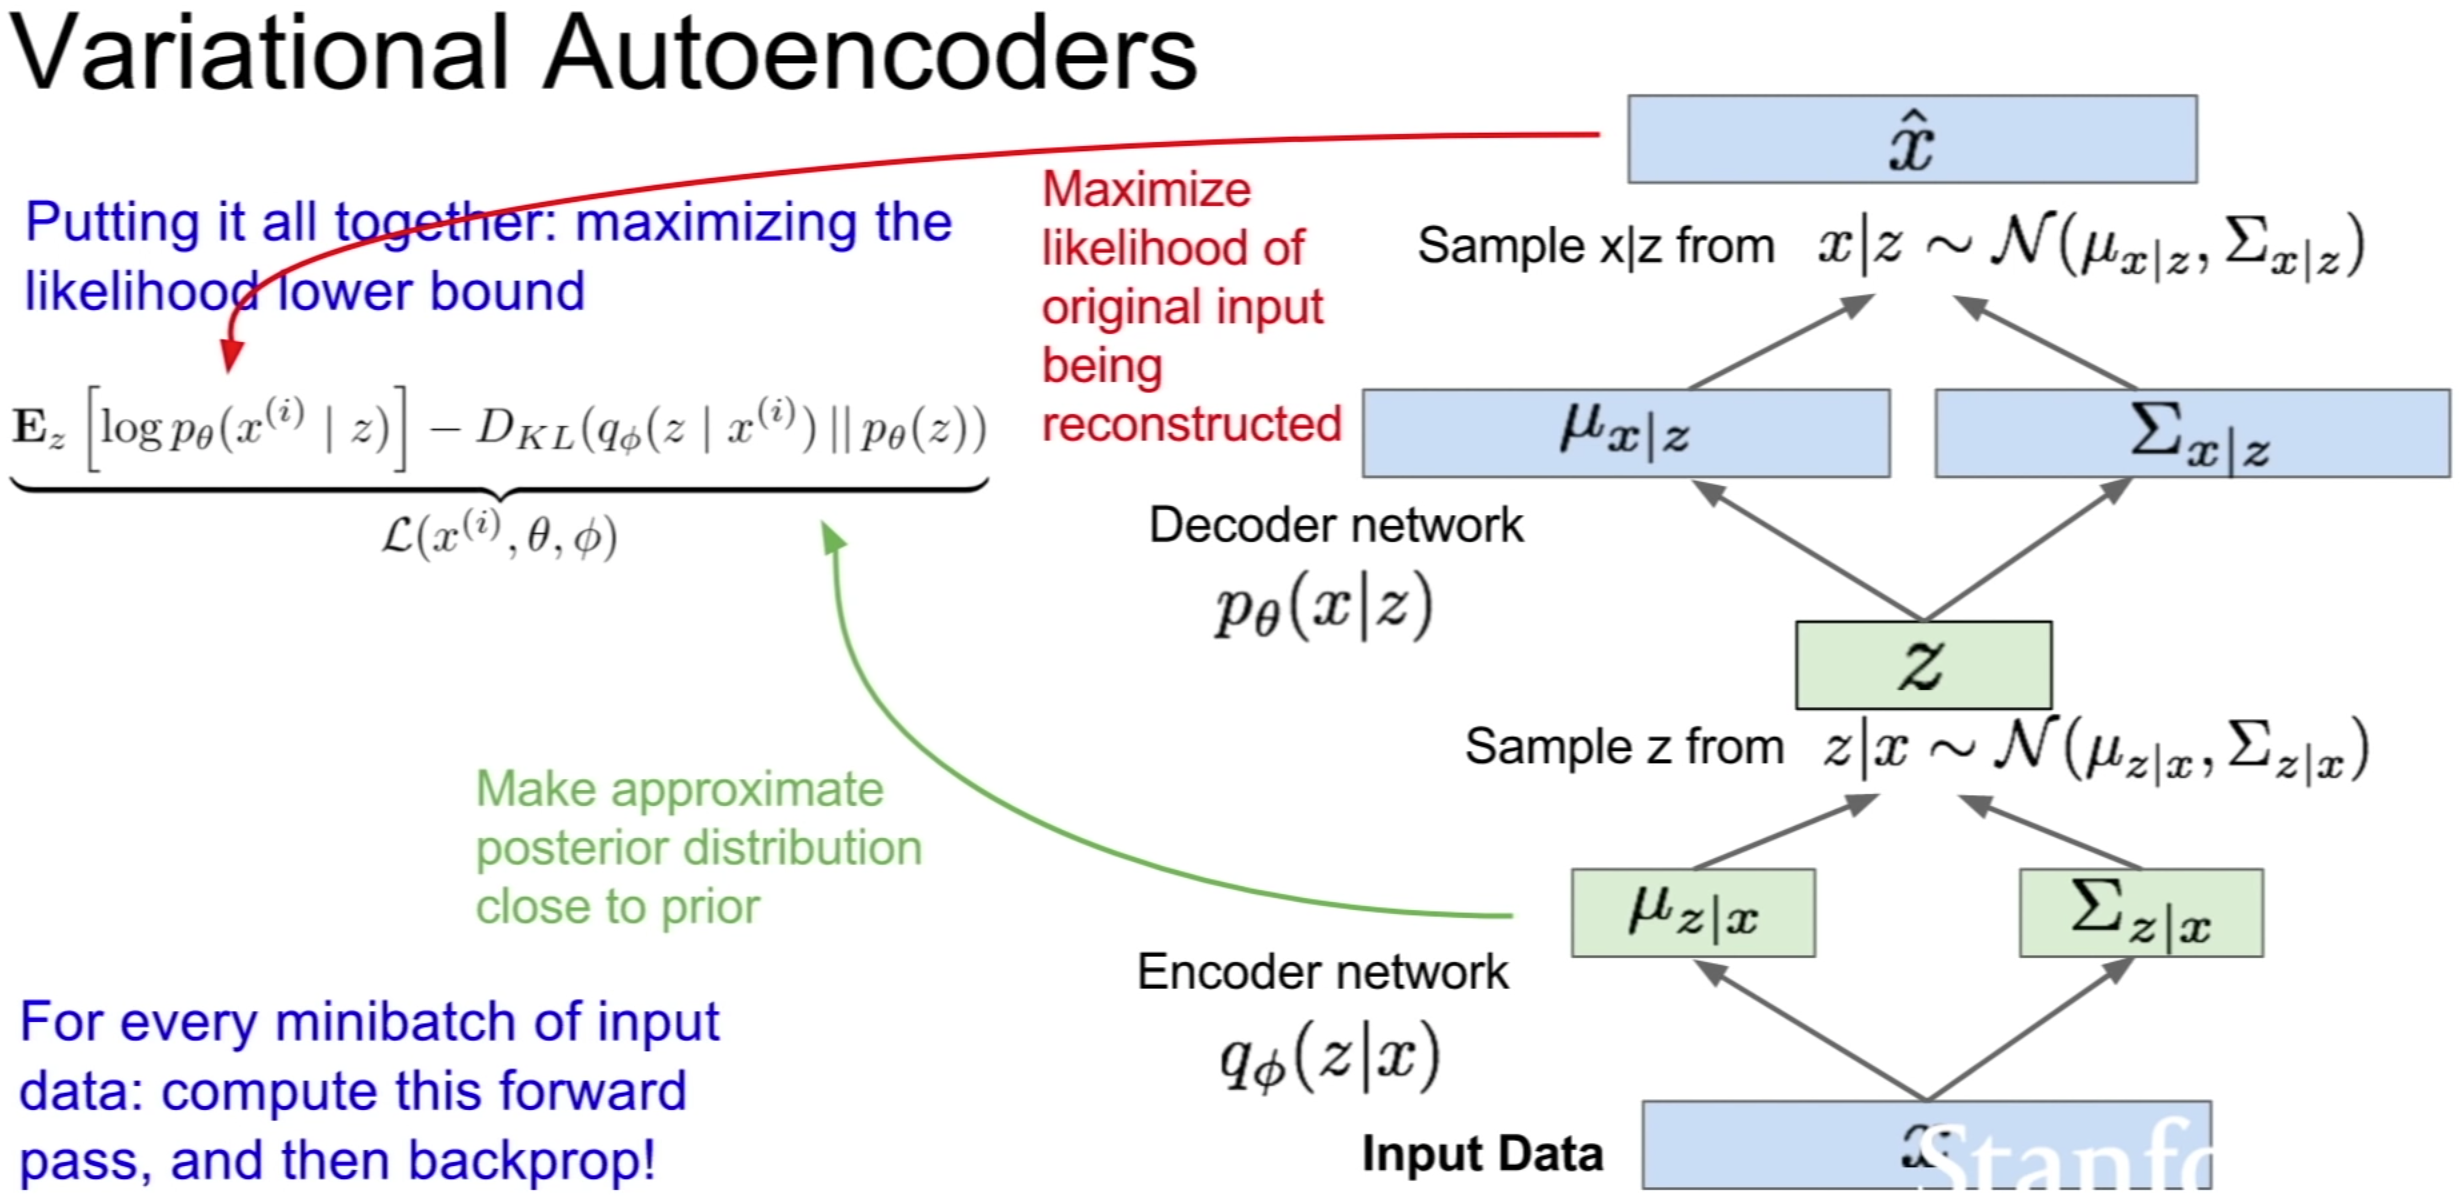
\includegraphics[width=1\linewidth]{%
img/VAE-forward-prop}
\end{center}

So, first we do the whole backpropagation. And then we just compute the updates
to the parameters $\theta$ and $\phi$ via backpropagation.

\todo{Show exactly what the losses are (1) and (2) (or do it as an exercise)}

\sep

\textbf{Generating Data} Here we just sample from the prior, and pass it through
the decoder network to get the posterior distribution's parameters, then we
sample from that one.


\subsection{Generative Adversarial Networks (GANs)}

GANs do not try to model a density function but directly aim to build a function
to generated data (implicit generative method). The whole optimization motivated
by a game-theoretic approach in a 2-player game. GANs sample from a simple
random noise distribution and try to learn a transformation (via a NN) to a data
distribution.

\sep

\Def[Discriminator $D$] must be a differentiable function parametrized by
$\theta_d$

$
\vx\stackrel{D}{\mapsto}\Prob{\vx \text{ comes  from true data distr.}}\in[0,1]
$

\ssep

\Def[Generator $G$] must be a differentiable function parametrized by $\theta_g$

$
\vz\sim\cN(\vmu,\MSigma)
\stackrel{G}{\mapsto}
\vx
\text{ (one falsified data sample)}
$ (one may also use another prior)

$\vz$ is sampled from the prior distr. over latent vars (source of randomness)

\sep

$D$ tries to make $D(G(\vz))$ near 0 (for fake data)

$D$ tries to make $D(\vx)$ near 1 ($\vx$ sampled from true data)

$G$ tries to make $D(G(\vz))$ near 1

\Com In some sense $G$ implicitly tries to make $D(\vx)$ near 0 (since it uses
the negative loss of $D$) see Minimax game VS Non-Saturating game.

\sep

\textbf{Minimax Game:} Both $D$ and $G$ try to minimize and maximize the same
value function:

\begin{gather*}
\begin{align*}
V(G,D)
&=\min_{G}\max_{D} \cR^{(D)}
\\
&=\min_{\theta_g}\max_{\theta_d}
\Exp[\vx\sim p_{\text{data}}]{\log(D_{\theta_d}(\vx))}
+
\Exp[\vz\sim p(\vz)]{\log(1-D_{\theta_d}(G_{\theta_g}(\vz)))}
\end{align*}
\end{gather*}

\todo{Write it in terms of cross-entropy!!}

$
\cR^{(D)}
=
-\frac{1}{2}
\Exp[\vx\sim p_{\text{data}}]{\log(D(\vx))}
-\frac{1}{2}
\underbrace{\Exp[\vz\sim \cN(\vmu,\MSigma)]{\log(1-D(G(\vz)))}}_{=
\Exp[\vx\sim p_{\text{generator}}]{\log(1-D(\vx))}}
$

$
\cR^{(G)}
=
-\cR^{(D)}
$ 

\begin{itemize}
  \item The loss $\cR^{(D)}$ is simply the cross-entropy between $D$'s
  predictions and the correct labels in the binary classification task (real/fake)
  \item The equilibrium of this game is saddle point of the discriminator loss
  \item If we look for this equilibrium the whole procedure resembles
  minimizing the Jensen-Shannon divergence between the true data distribution
  and the generator distribution.
  \item So $G$ minimizes the log-probability of $D$ being correct
\end{itemize}

\sep

\todo{Show Equivalence to Jensen Shannon Divergence}

\sep

\textbf{What is the solution $D(\vx)$ in terms of $p_{\text{data}}$ and
$p_{\text{generator}}$ at the equilibrium?}

In the equilibrium it must hold that the gradient of the discriminator is zero,
because the discriminator otherwise would improve (thus change) itself.

$
\frac{\partial \cR^{(D)}}{\partial D(\vx)}
=
-\frac{1}{2}
\Exp[\vx\sim p_{\text{data}}]{\frac{1}{D(\vx)}}
+\frac{1}{2}
\Exp[\vx\sim p_{\text{generator}}]{\frac{1}{1-D(\vx)}}
\mbeq 0
$

$
\Longleftrightarrow
\Exp[\vx\sim p_{\text{data}}]{\frac{1}{D(\vx)}}
=
\Exp[\vx\sim p_{\text{generator}}]{\frac{1}{1-D(\vx)}}
$

$
\Longleftrightarrow
\int_{\cX} p_{\text{data}}(\vx)\frac{1}{D(\vx)}\,d\vx
=
\int_{\cX} p_{\text{generator}}(\vx)\frac{1}{1-D(\vx)}\,d\vx
$

Recall: we can get rid of the integral as it is just a function operator. Using
the inverse of the operator, we can get rid of it and the solution constraints
on the optimal $D(\vx)$ still remain the same.

$
\Longleftrightarrow
p_{\text{data}}(\vx)\frac{1}{D(\vx)}
=
p_{\text{generator}}(\vx)\frac{1}{1-D(\vx)}
$

\begin{comment}
$
\Longleftrightarrow
p_{\text{data}}(\vx)\frac{1-D(\vx)}{D(\vx)}
=
p_{\text{generator}}(\vx)
$

$
\Longleftrightarrow
p_{\text{data}}(\vx)\frac{1}{D(\vx)} - p_{\text{data}}(\vx)
=
p_{\text{generator}}(\vx)
$

$
\Longleftrightarrow
p_{\text{data}}(\vx)\frac{1}{D(\vx)}
=
p_{\text{data}}(\vx) + p_{\text{generator}}(\vx) 
$

$
\Longleftrightarrow
\frac{1}{D(\vx)}
=
\frac{p_{\text{data}}(\vx)+p_{\text{generator}}(\vx)}{p_{\text{data}}(\vx)}
$

$
\Longleftrightarrow
D(\vx)
=
\frac{p_{\text{data}}(\vx)}{p_{\text{data}}(\vx) +
p_{\text{generator}}(\vx)} $
\end{comment}

Then we get the following stationarity
condition: The optimal $D(\vx)$ for any $p_{\text{data}}(\vx)$ and
$p_{\text{generator}}(\vx)$ is always

$
D(\vx)
=
\frac{p_{\text{data}}(\vx)}{p_{\text{data}}(\vx) + p_{\text{generator}}(\vx)}
$

Note that by stationarity condition we mean that this must hold in the
Nash equilibrium (where both players stop adapting themselves).

Estimating this ratio using supervised learning is the key approximation
mechanism used by GANs.



What assumptions are needed to obtain this solution?

We need to assume that both densities are nonzero everywhere. If we don't make
this assumption then there's this issue that the discriminator's input space
might never be sampled during its training process. Then these points would have
an undefined behaviour since they're never trained.

\sep

\textbf{Training Procedure:} Use SGD-like algorithm of choice (ADAM) on two
minibatches simultaneously. At each iteration, we choose:
\begin{itemize}
  \item a minibatch of true data samples
  \item a minibatch of noise vectors to produce minibatch generated samples
\end{itemize}
Then compute both losses and perform gradient updates.

$\theta_d^{t+1}\gets\theta_d^t-\eta_t\nabla_{\theta_d}\cR^{(D)}(\theta_d)$

$\theta_g^{t+1}\gets\theta_g^t-\eta_t\nabla_{\theta_g}\cR^{(G)}(\theta_g)$

Optional: run $k\geq 1$ update steps of $D$ for every iteration (and only
$1$ update step for $G$).

So we alternate between
\begin{itemize}
  \item \textbf{Gradient ascent} on $D$\\
  $
\max_{\theta_d}
\Exp[\vx\sim p_{\text{data}}]{\log(D_{\theta_d}(\vx))}
+
\Exp[\vz\sim p(\vz)]{\log(1-D_{\theta_d}(G_{\theta_g}(\vz)))}
  $
  \item \textbf{Gradient descent} on $G$\\
  $
\min_{\theta_g}
\Exp[\vz\sim p(\vz)]{\log(1-D_{\theta_d}(G_{\theta_g}(\vz)))}
  $
\end{itemize}

\ssep

Note that this training algorithm uses a heuristically motivated loss (that is
a bit different) for the generator to have better gradients when the
discriminator is good:

\begin{center}
  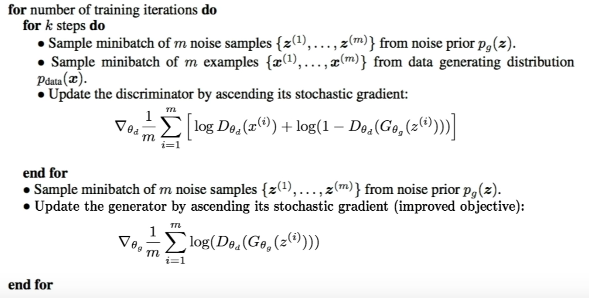
\includegraphics[width=1\linewidth]{%
img/GAN-training}
\end{center}

\sep

\todo{From here on until end was not treated in lecture. See comments}

\begin{comment}
What prevents the generator from just learning about one specific true image and
then constantly outputting it? (as it would be indistinguishable)

If we're able to correctly play the Minimax game then $G$ is not able to
consistently fool $D$ by always generating the same sample. $D$ would learn to
recognize that sample and reject it as fake.

\todo{Also write about mode collapse.}

\sep

Improvements of this model could use importance sampling in both latent and true
data space to improve $G$.

\sep

\textbf{Non-Saturating Game}

Here we change $G$'s loss as follows

$
\cR^{(G)}
=
-\frac{1}{2}\Exp[\vz\sim\cN(\vmu,\MSigma)]{D(G(\vz))}.
$

Hence the equilibrium is no longer describable with a single loss. Now the
generator just maximizes the log-probability of the discriminator being
mistaken. Heuristically motivated: $G$ can still learn even when
$D$ successfully rejects all generator samples.

The problem with the Minimax game is that when $D$ becomes to smart, the
gradient for $G$ goes away.

\sep
\end{comment}

\end{multicols*}
\end{landscape}
\end{document}